\section{Прогнозирование временных рядов}

\subsection{Временные ряды}

Временным рядом называется последовательность значений признака y, измеряемого 
через постоянные временные интервалы:

\begin{equation*}
    y_1, \dots, y_T, \dots, \quad y_t \in \mathbb{R}.
\end{equation*}
В этом определении нужно обратить внимание на то, что временные интервалы между 
измерениями признака постоянны.\\[-0.5em]

\begin{figure}[h!]
    \centering
    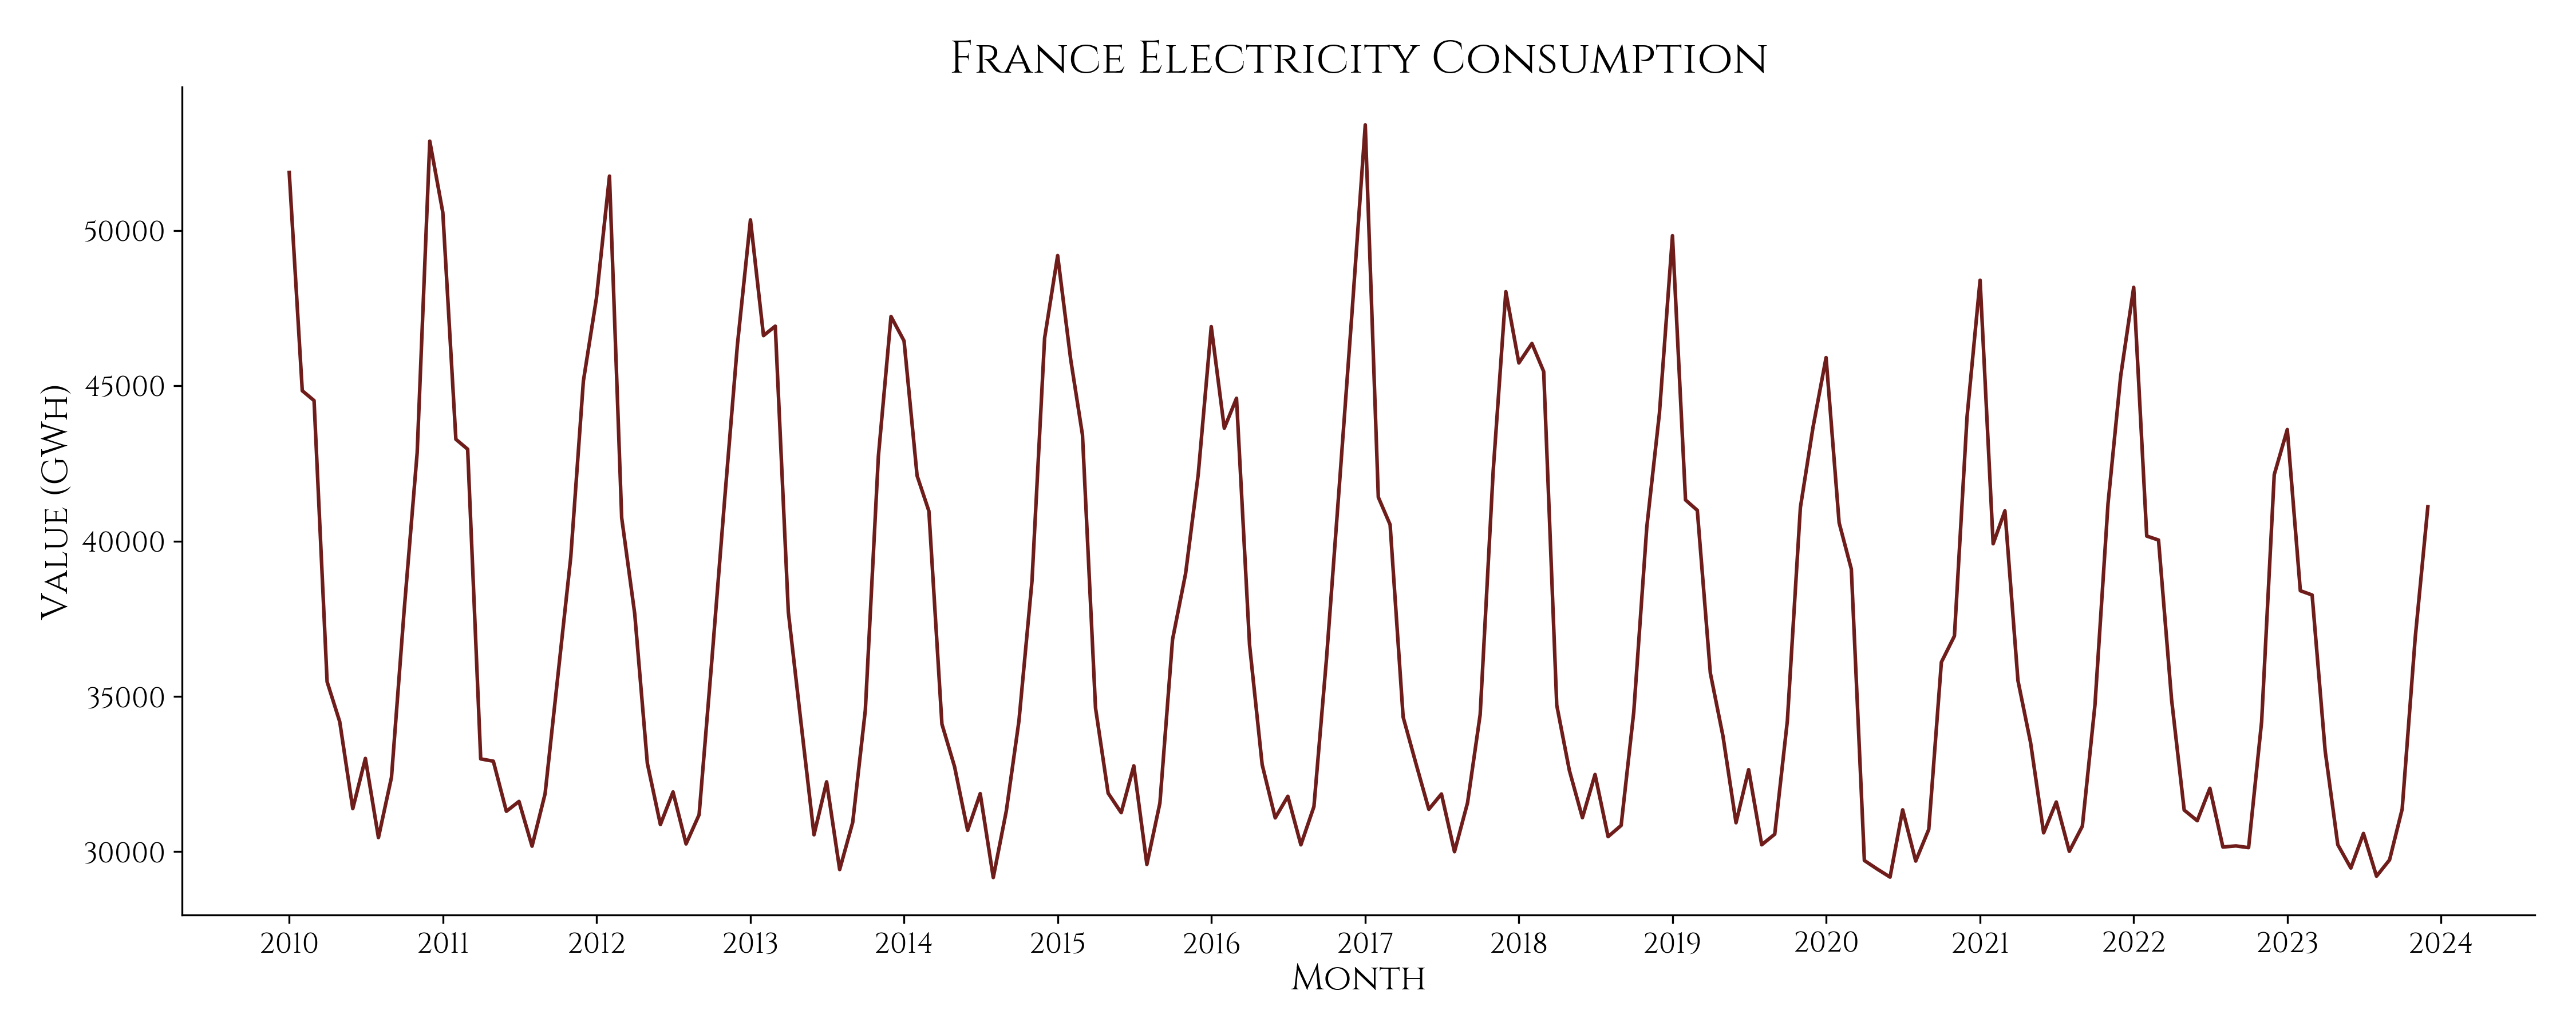
\includegraphics[width=1\textwidth, height=1\textheight, keepaspectratio]{time_series_example_France}
    \caption{Ежемесячное потребление электричества во Франции. 
    Построено программой по адресу (листинг \ref{lst:time_series_example_France}).}
    \label{fig:time_series_example_France}
\end{figure}

Временные ряды изобилуют в таких
областях, как экономика, бизнес, инженерия, естественные науки 
(особенно геофизика и метеорология), а также социальные науки.

Примеры временных рядов - это ряды с  
ежемесячной последовательностью объемов отгруженных с завода товаров, 
еженедельными данными о количестве дорожно-транспортных происшествий, 
ежедневными объемами осадков, почасовыми наблюдениями за химическеми 
выбросами. Ещё один пример временного ряда 
(показан на рисунке \ref{fig:time_series_example_France}) — это реальное 
ежемесячное потребление электричества во Франции.

\subsubsection{Прогнозирование временного ряда \cite{TSA_Box}}

Информация о доступных наблюдениях в момент времени $t$ временного ряда, 
используемая для предсказания его значения в некотором будущем $t+l$ может 
предоставить фундамент для планирования в бизнесе и экономике, контроля продукции, 
оптимизации индустриальных процессов и так далее. Здесь $l$ - это, так называемый, 
\textit{горизонт прогнозирования}, который меняется от задачи к задаче.

Предположим, что наблюдения - \textit{дискретные}, равноудаленные друг от друга величины. 
Например в задаче прогнозирования продаж, продажи $z_t$ в текущий месяц $t$ и продажи 
$z_{t-1}, z_{t-2}, z_{t-3}, ...$ в предыдущие месяцы можно использовать для 
прогнозирования горизонта в $l = 1, 2, 3, ..., 12$ месяцев. Обозначим за $\hat{z}_t (l)$ 
прогноз, составленный в \textit{момент времени} $t$ для продаж $z_{t+l}$ в некотором будущем $t+l$, т.е.
с \textit{горизонтом прогнозирования} $l$. Функция $\hat{z}_t (l)$, прогнозирующая в момент времени 
$t$ для всех будущих горизнтов прогнозирования, на основе доступной информации о 
текущем и предыдущих значениях $z_t, z_{t-1}, z_{t-2}, z_{t-3}, ...$ на протяжении времени $t$, 
называется \textit{функцией прогнозирования} в момент времени $t$. Основная задача 
прогнозирования временных рядов заключается в том, чтобы найти функцию прогнозирования с 
наименьшим средним квадратом отклонений $z_{t+l} - \hat{z}_t (l)$ между истинными и 
спрогнозированными значениями для каждого из \textit{горизонтов прогнозирования} $l$. 

В добавок к нахождению наилучших прогнозов, также необходимо указать их точность, так 
чтобы, например, можно было рассчитать риски, ассоциированные с решениями, принятыми на 
их основе. Точность прогнозов можно выразить в качестве \textit{доверительных интервалов} 
с каждой стороны прогноза. Эти интервалы могут быть рассчитаны для любого удобного набора 
вероятностей, например, 50 и 95\%. Они указывают вероятность попадания спрогнозированной 
величины в данный интервал. За иллюстрацией обратимся к рис. \ref{fig:time_series_forecast_probability_limit}, 
на котором изображены последние 20 значений временного ряда, кульминирующие в момент времени $t$. 
Также представлены прогнозы, сделанные в момент времени $t$ с горизонтами прогнозирования 
$l = 1, 2, ..., 13$, вместе с 50\% доверетильными интервалами.

\begin{figure}[h!]
    \centering
    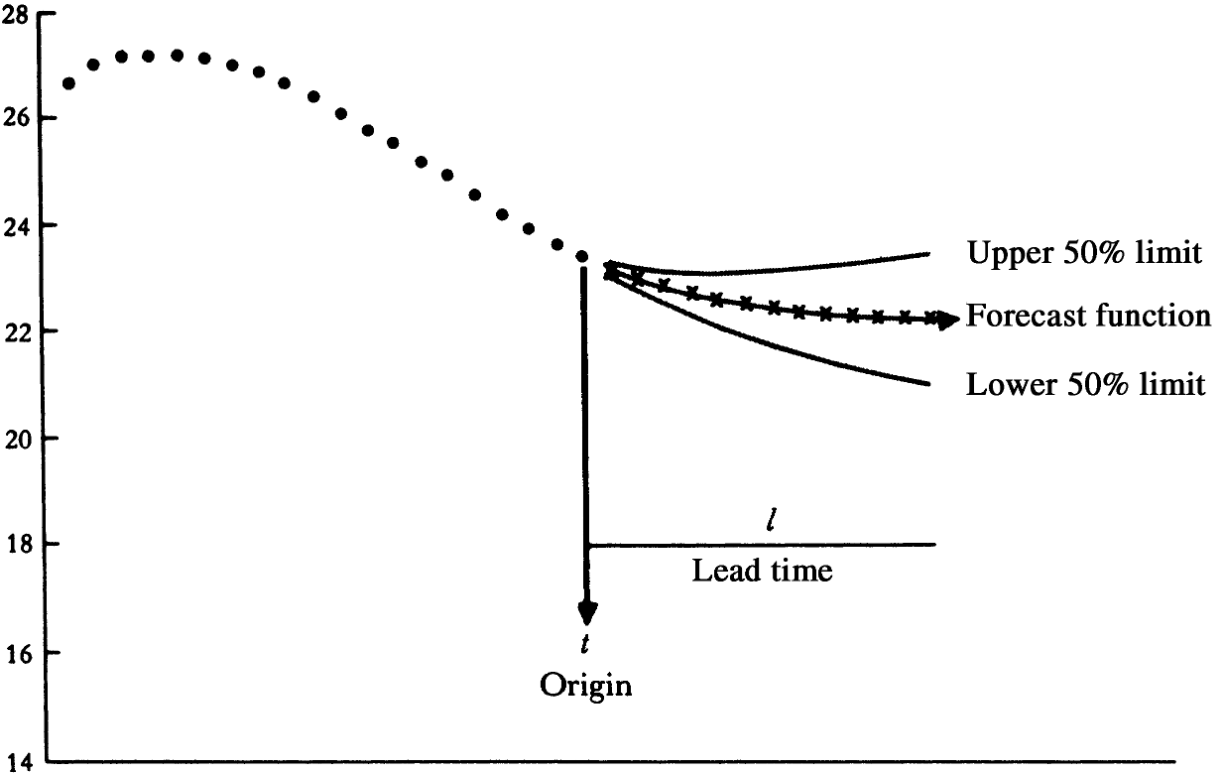
\includegraphics[width=0.8\textwidth, height=0.8\textheight, keepaspectratio]{time_series_forecast_probability_limit}
    \caption{Значения временного ряда с прогнозирующей функцией и 50\% доверетильными интервалами.}
    \label{fig:time_series_forecast_probability_limit}
\end{figure}

\subsubsection{Главная особенность временных рядов}

Чаcто, в задачах регрессионного анализа и машинного обучения, в качестве анализируемых 
данных берутся простые выборки, построенные из независимо одинаково распредленных 
наблюдений. В задаче анализа временных рядов всё с точностью наоборот: 
предполагается, что данные в прошлом каким-то образом связаны с данными в будущем. 
Чем сильнее они связаны, тем больше имеется информации о поведении временного ряда 
в будущем и тем точнее можно сделать прогноз. 

Полезно снова рассмотреть данные о реальном ежемесячном потреблении электричества во Франции 
(рис. \ref{fig:time_series_example_France}). Видно, что на графике изображена не простая 
выборка (измерения не являются независимыми и одинаково распределёнными), а сложный, 
структурированный процесс. Выявив структуру этого процесса, можно учесть её в
прогнозирующей модели и построить действительно точный прогноз.

\subsubsection{Компоненты временных рядов}

Полезно рассмотреть несколько понятий, которыми можно описать поведение временных рядов:

\begin{itemize}
    \item Тренд — плавное долгосрочное изменение уровня ряда. Эту характеристику можно получить, наблюдая
    ряд в течение достаточно долгого времени.
    \item Сезонность — циклические изменения уровня ряда с постоянным периодом. В данных о ежемесячном 
    потреблении электричества во Франции (рис. \ref{fig:time_series_example_France}) очень хорошо видны подобные 
    сезонные колебания: признак всегда принимает максимальное значение зимой, а минимальное — летом. 
    Это легко объяснить тем, что летом электричества необходимо меньше всего, это самый тёплый сезон 
    во Франции. В целом профиль изменения потребления электричества внутри года остаётся более-менее 
    постоянным.
    \item Цикл — изменение уровня ряда с переменным периодом. Такое поведение часто встречается в рядах,
    связанных с продажами, и объясняется циклическими изменениями экономической активности. В эко-
    номике выделяют циклы длиной 4 - 5 лет, 7 - 11 лет, 45 - 50 лет и т. д. Другой пример ряда с такой
    характеристикой — это солнечная активность, которая соответствует, например, количеству солнечных
    пятен за день. Она плавно меняется с периодом, который составляет несколько лет, причём сам период
    также меняется во времени.
    \item Ошибка — непрогнозируемая случайная компонента ряда. Сюда включены все те характеристики временного ряда, 
    которые сложно измерить (например, слишком слабые).
\end{itemize}

\subsection{Автокорреляция}

Одной из важнейших характеристик временного ряда является автокорреляция. Автокорреляцией 
назвается математическая репрезентация степени \guillemotleft схожести\guillemotright {} между 
исходным рядом и его версией, сдвинутой на некоторый интервал, называемый лагом. Концептуально 
это похоже на корреляцию Пирсона между двумя временными рядами, только автокорреляция рассматривает 
один и тот же ряд дважды. \\

Стоит напомнить, что коэффициент корреляции, а значит и автокорреляции может быть равен 0 при наличии сильной, 
но нелинейной зависимости (рис. \ref{fig:non_linear_correlation_example}) \cite{pml1Book}.\\

\begin{figure}[h!]
    \centering
    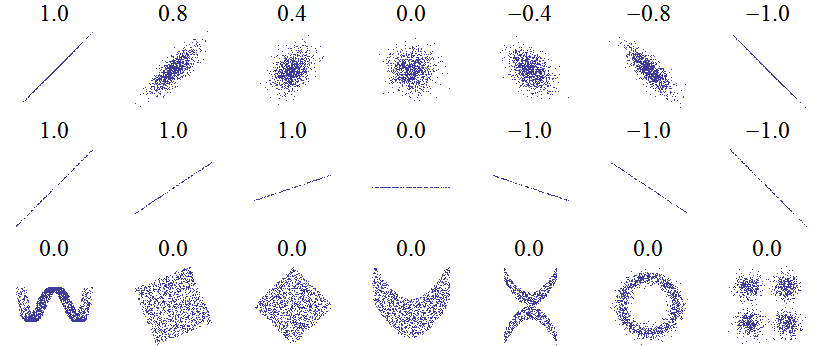
\includegraphics[width=0.9\textwidth, height=0.9\textheight, keepaspectratio]{non_linear_correlation_example}
    \caption{Несколько наборов точек (x, y) и коэффициент корреляции x и y
    для каждого набора. Отметим, что корреляция отражает зашумленность и направление 
    линейной зависимости (верхний ряд), но не отражает ее угловой
    коэффициент (средний ряд), а также многие аспекты нелинейных связей (нижний ряд). 
    (Примечание: на рисунке в центре угловой коэффициент равен 0, но
    в этом случае коэффициент корреляции не определен, потому что дисперсия Y
    нулевая.)}
    \label{fig:non_linear_correlation_example}
\end{figure}

\subsubsection{Автокорреляция, её вычисление}

Количественной характеристикой сходства между значениями ряда в соседних точках является 
автокорреляционная функция (или просто автокорреляция), которая задаётся следующим соотношением:\\

\begin{equation*}
    r_l \defeq \cfrac{\mathbb{E}[(y_t - \mathbb{E}_y)(y_{t+l} - \mathbb{E}_y)]}{\mathbb{V}_y},
\end{equation*}
где количество отсчётов, на которое сдвинут ряд, называется лагом автокорреляции $(l)$.\\
Можно заметить сходство с корреляцией Пирсона:

\begin{equation*}
    \rho \defeq \text{corr}[X, Y] \defeq 
    \cfrac{\text{Cov}[X, Y]}{\sqrt{\mathbb{V}[X]\mathbb{V}[Y]}}, \qquad 
    \text{Cov}[X, Y] \defeq \mathbb{E}[(X - \mathbb{E}[X])(Y - \mathbb{E}[Y])]
\end{equation*}

Значения, принимаемые автокорреляцией такие же, как и у коэффициента 
Пирсона: $r_l \in [-1, 1]$. Вычислить автокорреляцию по выборке можно, заменив в формуле 
математическое ожидание на выборочное среднее, а дисперсию — на выборочную дисперсию.

\subsection{Визуализация временных рядов}

В анализе временных рядов огромную роль играет их визуализация. 
Графики \guillemotleft сырых\guillemotright {} данных могут предоставить такие 
важные сведения о временном ряде, как: тренды, циклы, сезонность и прочие структуры, 
важные для подбора модели предсказания. \\

Далее различные методы графического анализа будут (если не указано иное) 
демонстрироваться 
на примере данных о суммарном объёме продаж красного вина в Австралии за
месяц на протяжении 15 лет (рис. \ref{fig:time_series_wine}).

\begin{figure}[h!]
    \centering
    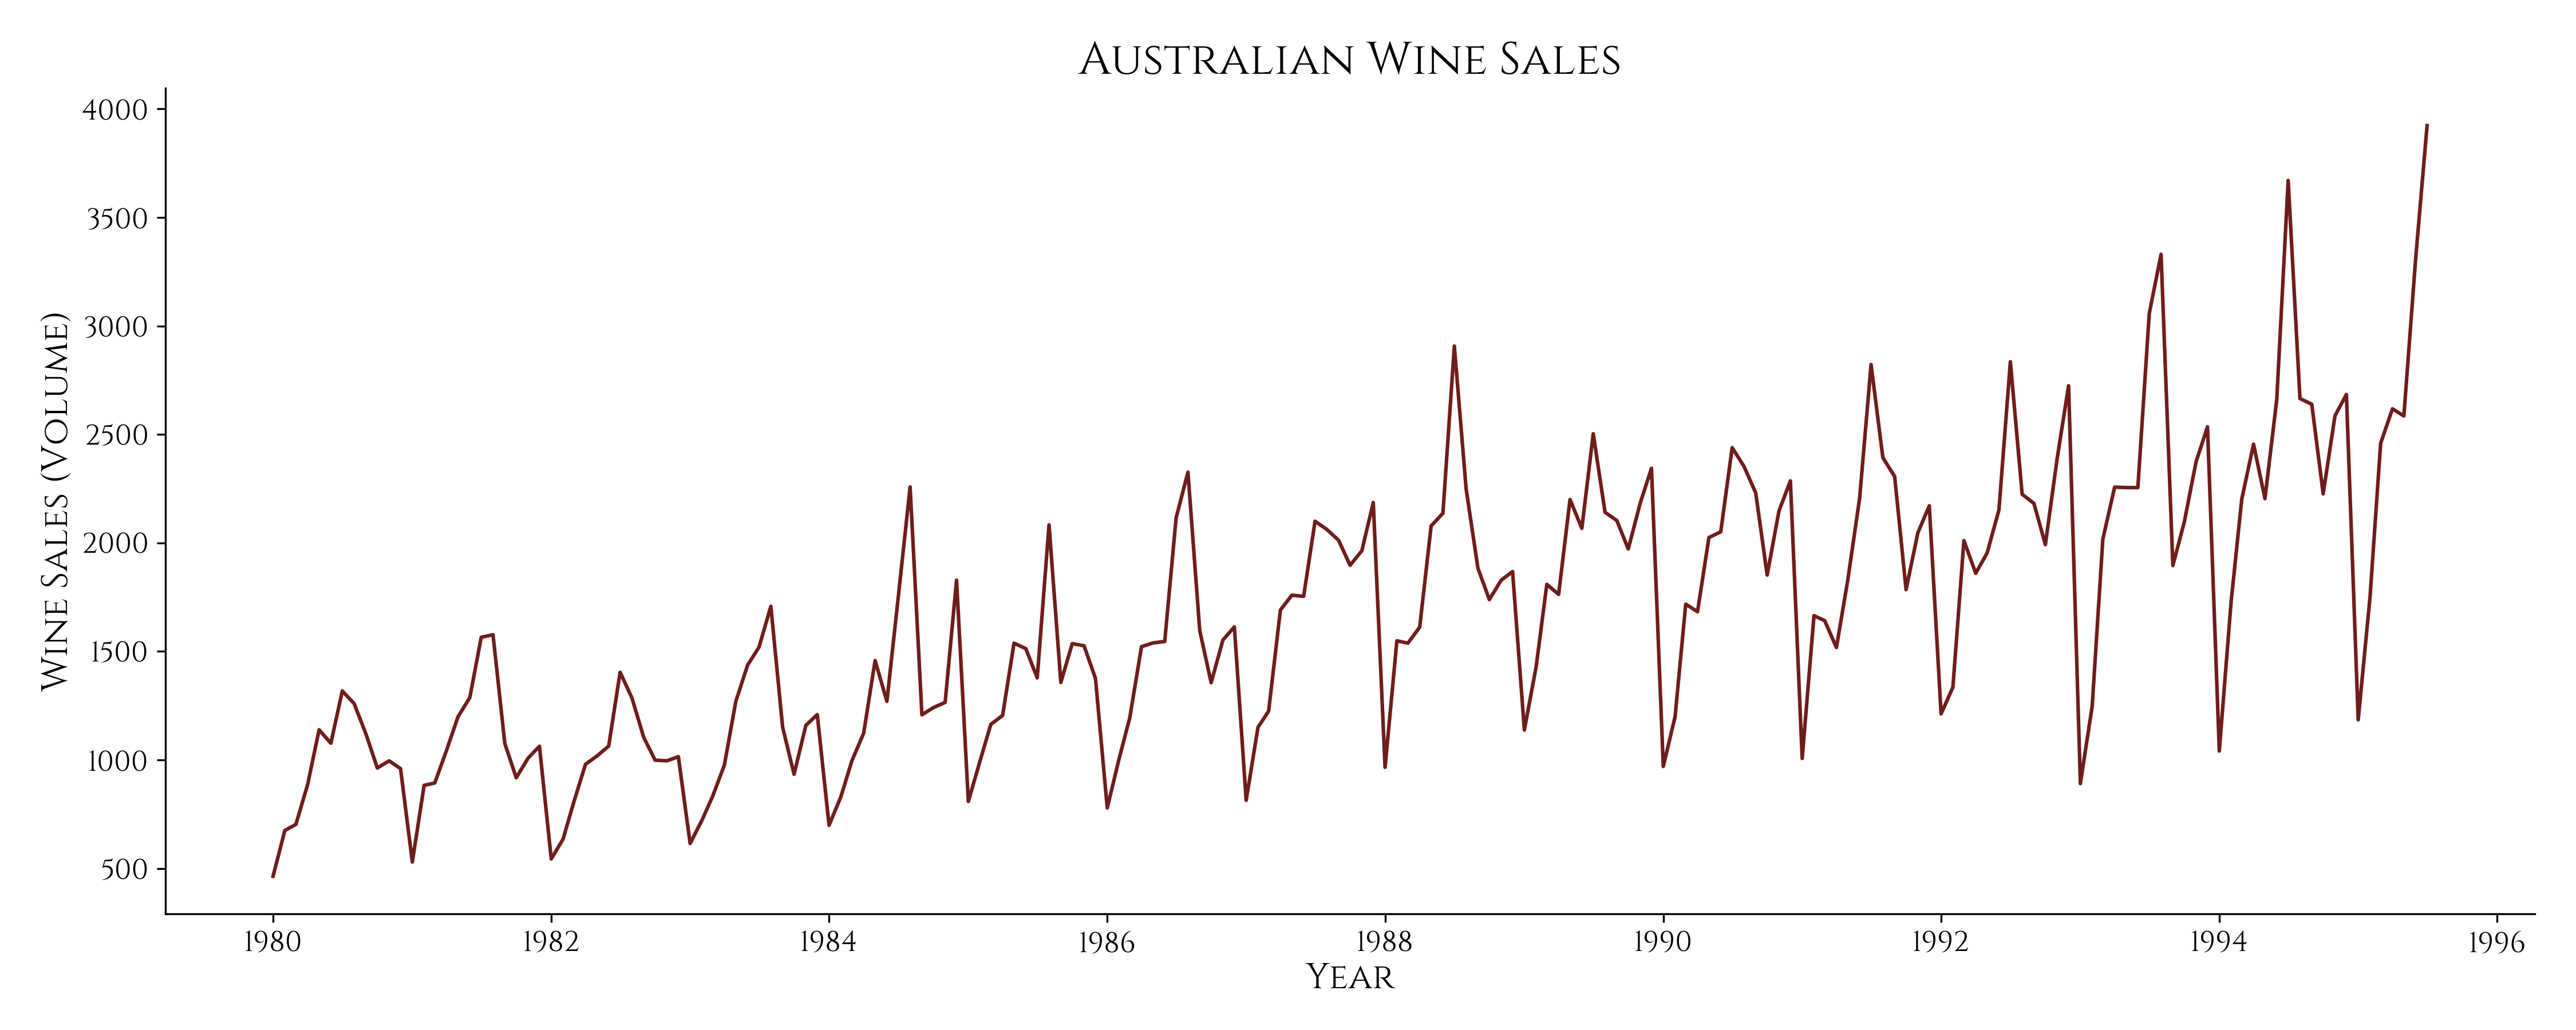
\includegraphics[width=1\textwidth, height=1\textheight, keepaspectratio]{time_series_example_wine}
    \caption{Месячный объём продаж красного вина в Австралии, в бутылках. 
    Построено программой по адресу (листинг \ref{lst:time_series_example_wine}).}
    \label{fig:time_series_wine}
\end{figure}

Этот ряд обладает ярко выраженной годовой сезонностью: максимум продаж за год 
приходится на декабрь, а затем, в январе, происходит существенное падение.

\subsubsection{Линейный график}

Наверное самым популярным из методов визуализации является линейный график (line plot), 
который, к слову, уже был ранее не раз продемонстрирован 
(см. рис. \ref{fig:time_series_example_France}, рис. \ref{fig:time_series_wine}, 
рис. \ref{fig:time_series_example_aep}). \\

Плотные графики иногда бывает полезно изобразить сгруппировав 
грaфики одного и того же временного ряда, но в разные промежутки времени, так например 
посмотрим на график ежечасового потребления электричества в Америке за 2009 год 
(рис. \ref{fig:time_series_example_aep}) 
в каждый месяц:

\begin{figure}[h!]
    \centering
    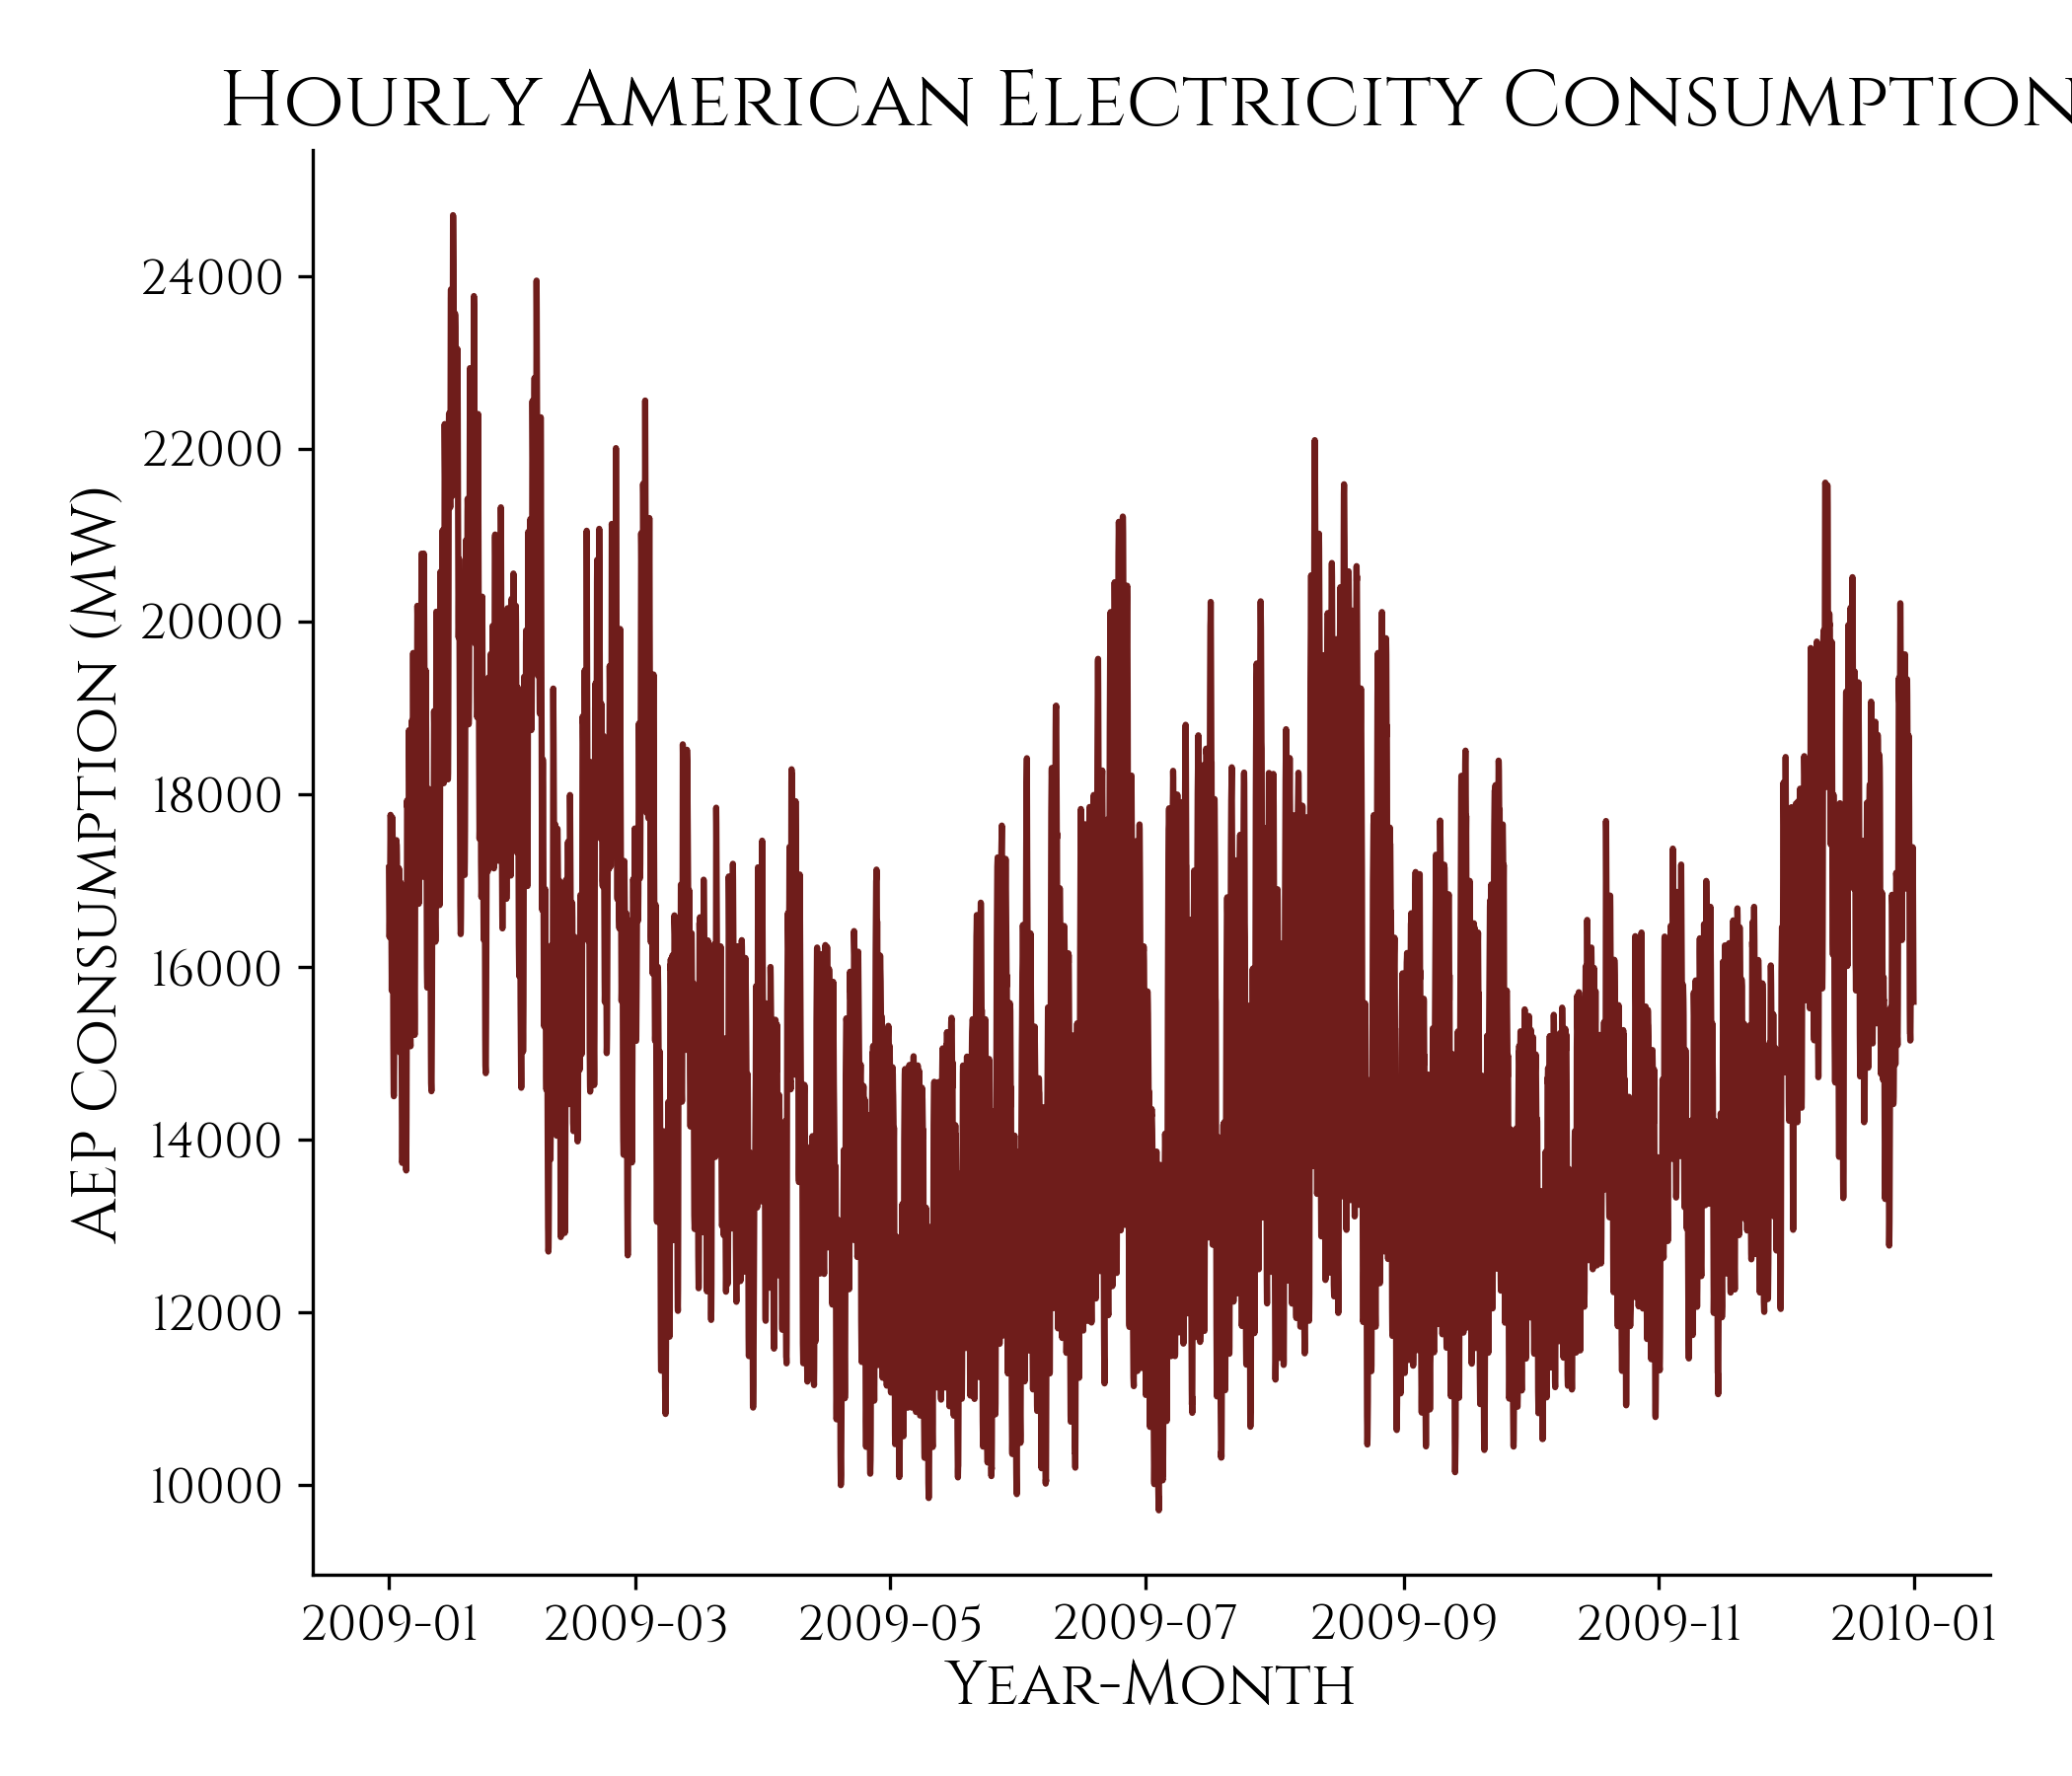
\includegraphics[width=0.8\textwidth, height=0.8\textheight, keepaspectratio]{time_series_example_aep}
    \captionof{figure}{Ежечасовое потребление электричества в Америке за 2009 год. 
    Построено программой по адресу 
    (листинг \ref{lst:time_series_example_aep}).}
    \label{fig:time_series_example_aep}
\end{figure}

\newpage

\begin{figure}[h!]
    \centering
    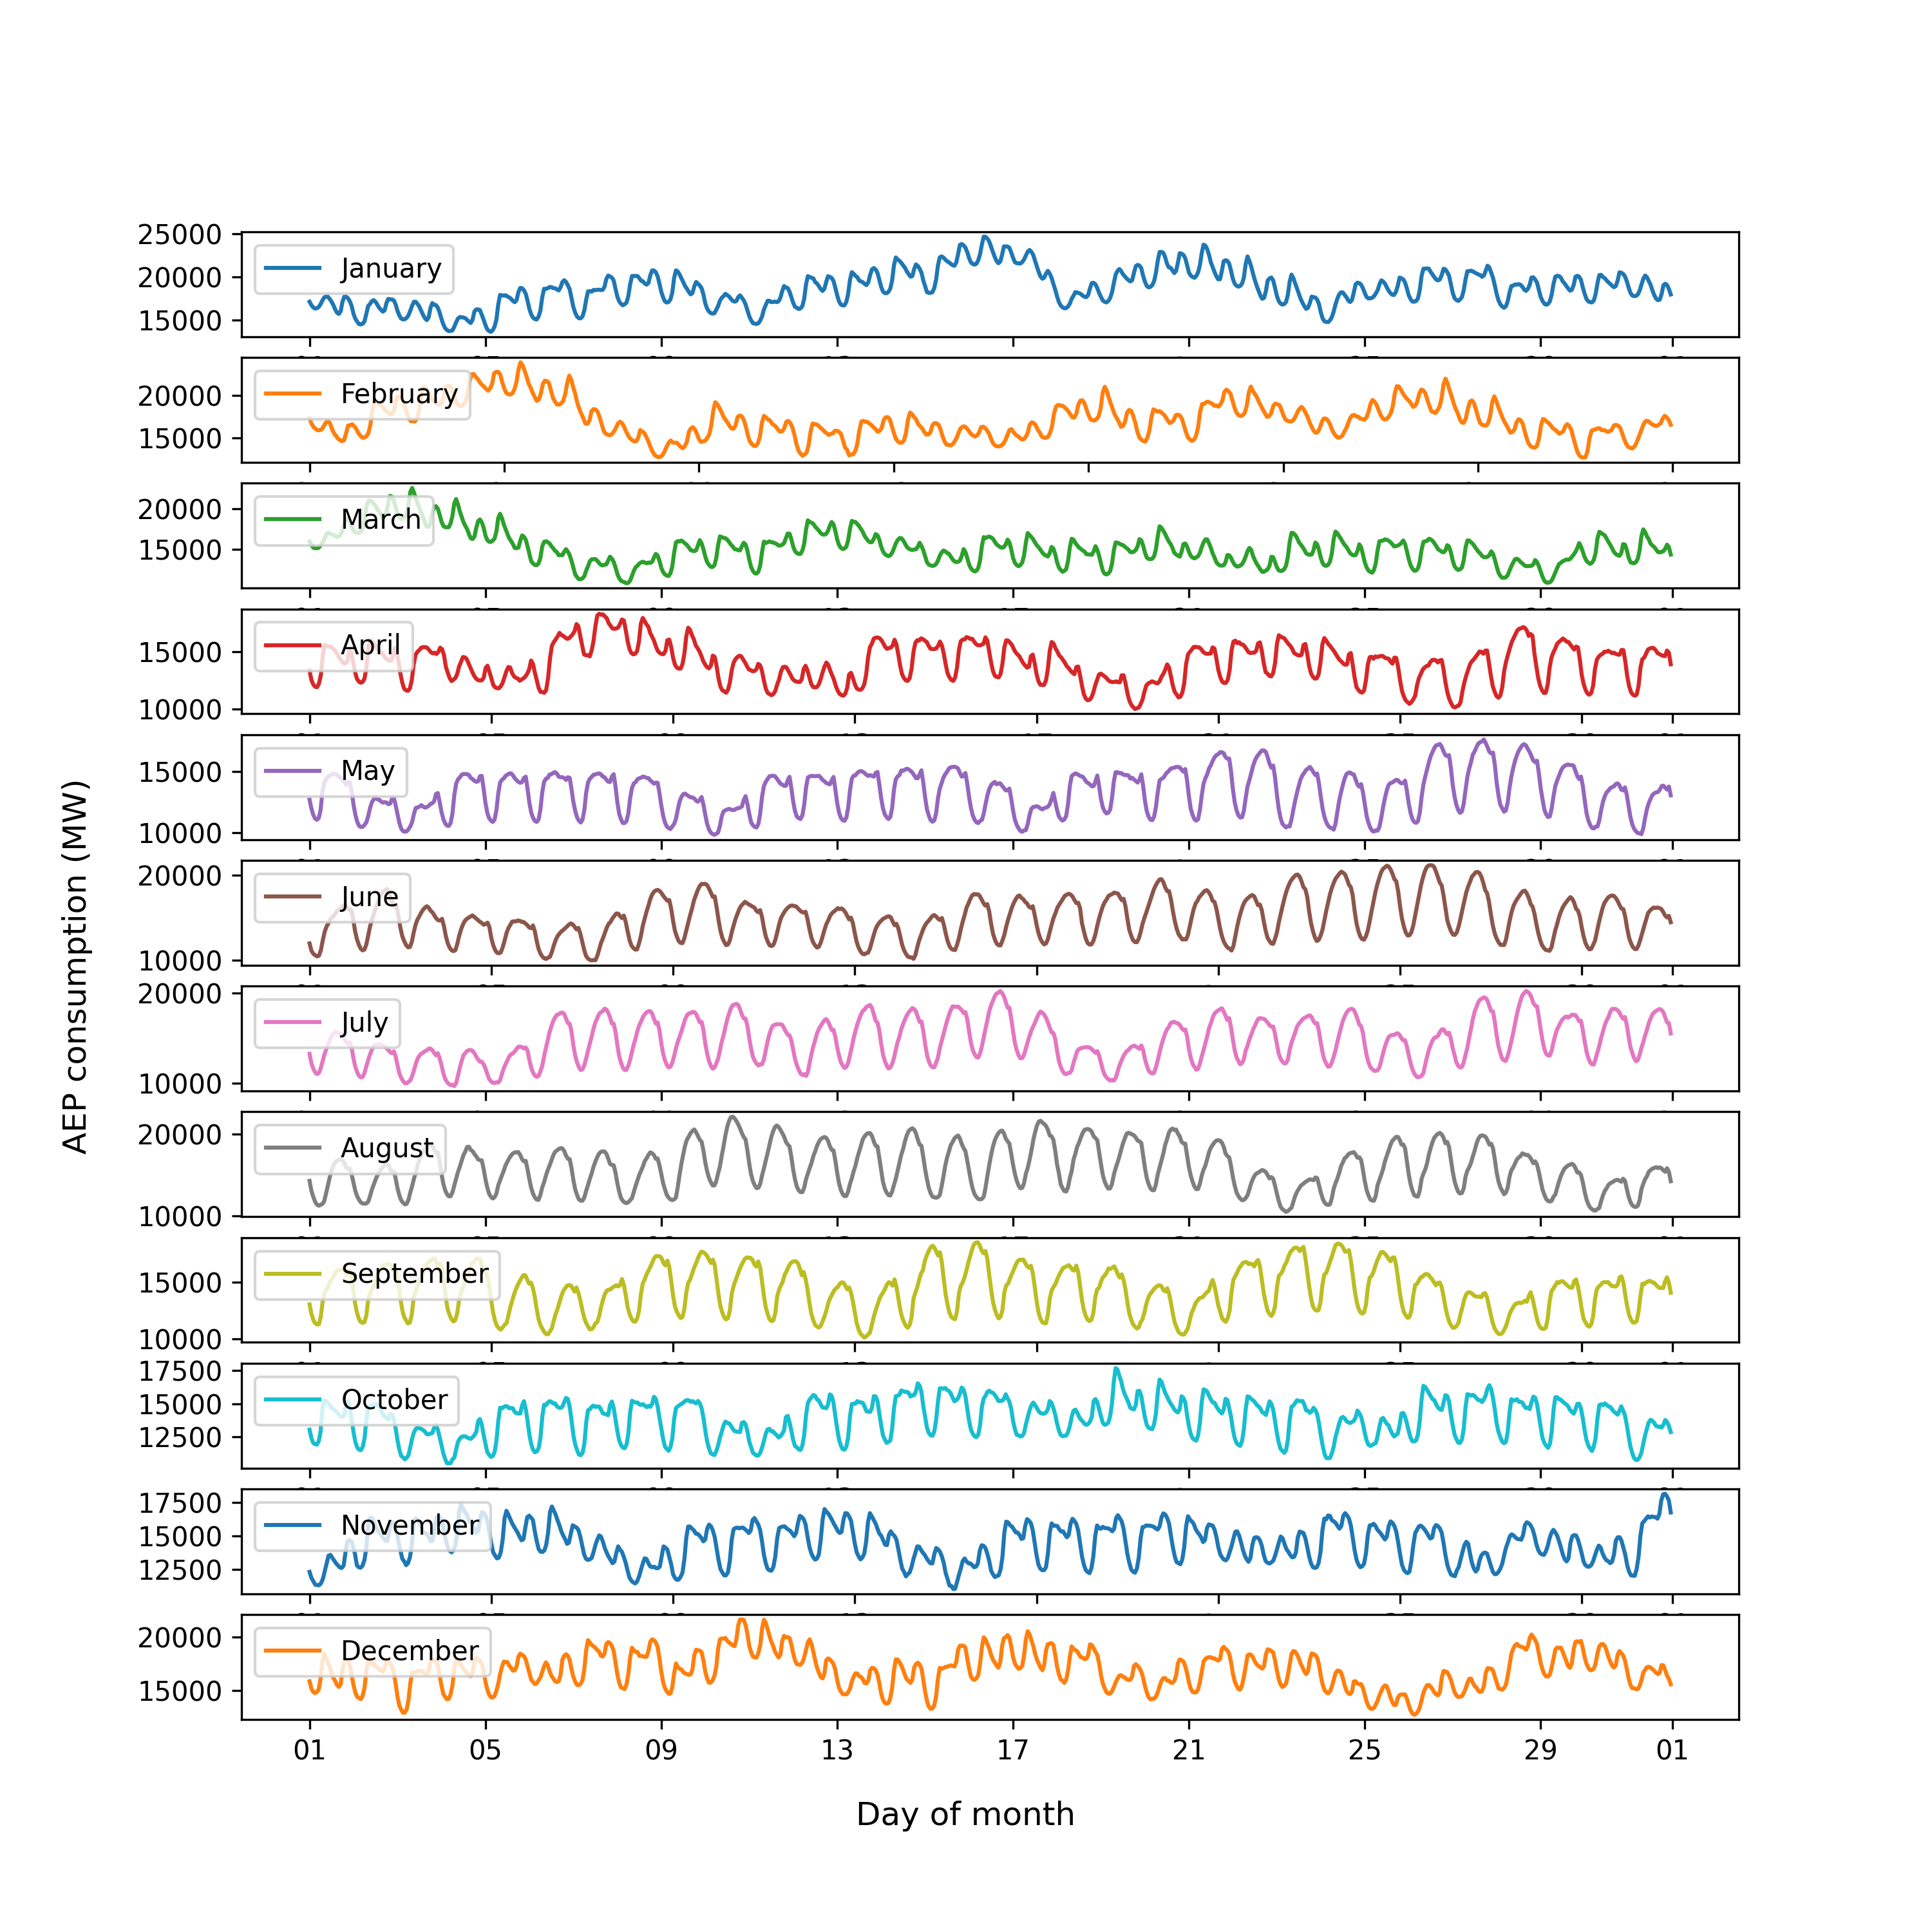
\includegraphics[width=1\textwidth, height=1\textheight, keepaspectratio]{time_series_example_aep_grouped}
    \captionof{figure}{Ежечасовое потребление электричества в Америке за 2009 год 
    в каждом месяце. Построено программой по адресу 
    (листинг \ref{lst:time_series_example_aep_grouped}).}
    \label{fig:time_series_example_aep_grouped}
\end{figure}

\subsubsection{Гистограмма и график плотности}

Другим не менее важным методом визуализации данных является визуализация 
их распределения. 
Некоторые линейные модели прогнозирования временных рядов ожидают 
\guillemotleft хороших\guillemotright {} данных (например нормальное распределение). 
Графики позволяют дать быструю первоначальную оценку типу распределения.

\begin{center}
    \begin{minipage}{0.4\textwidth}
        \centering
        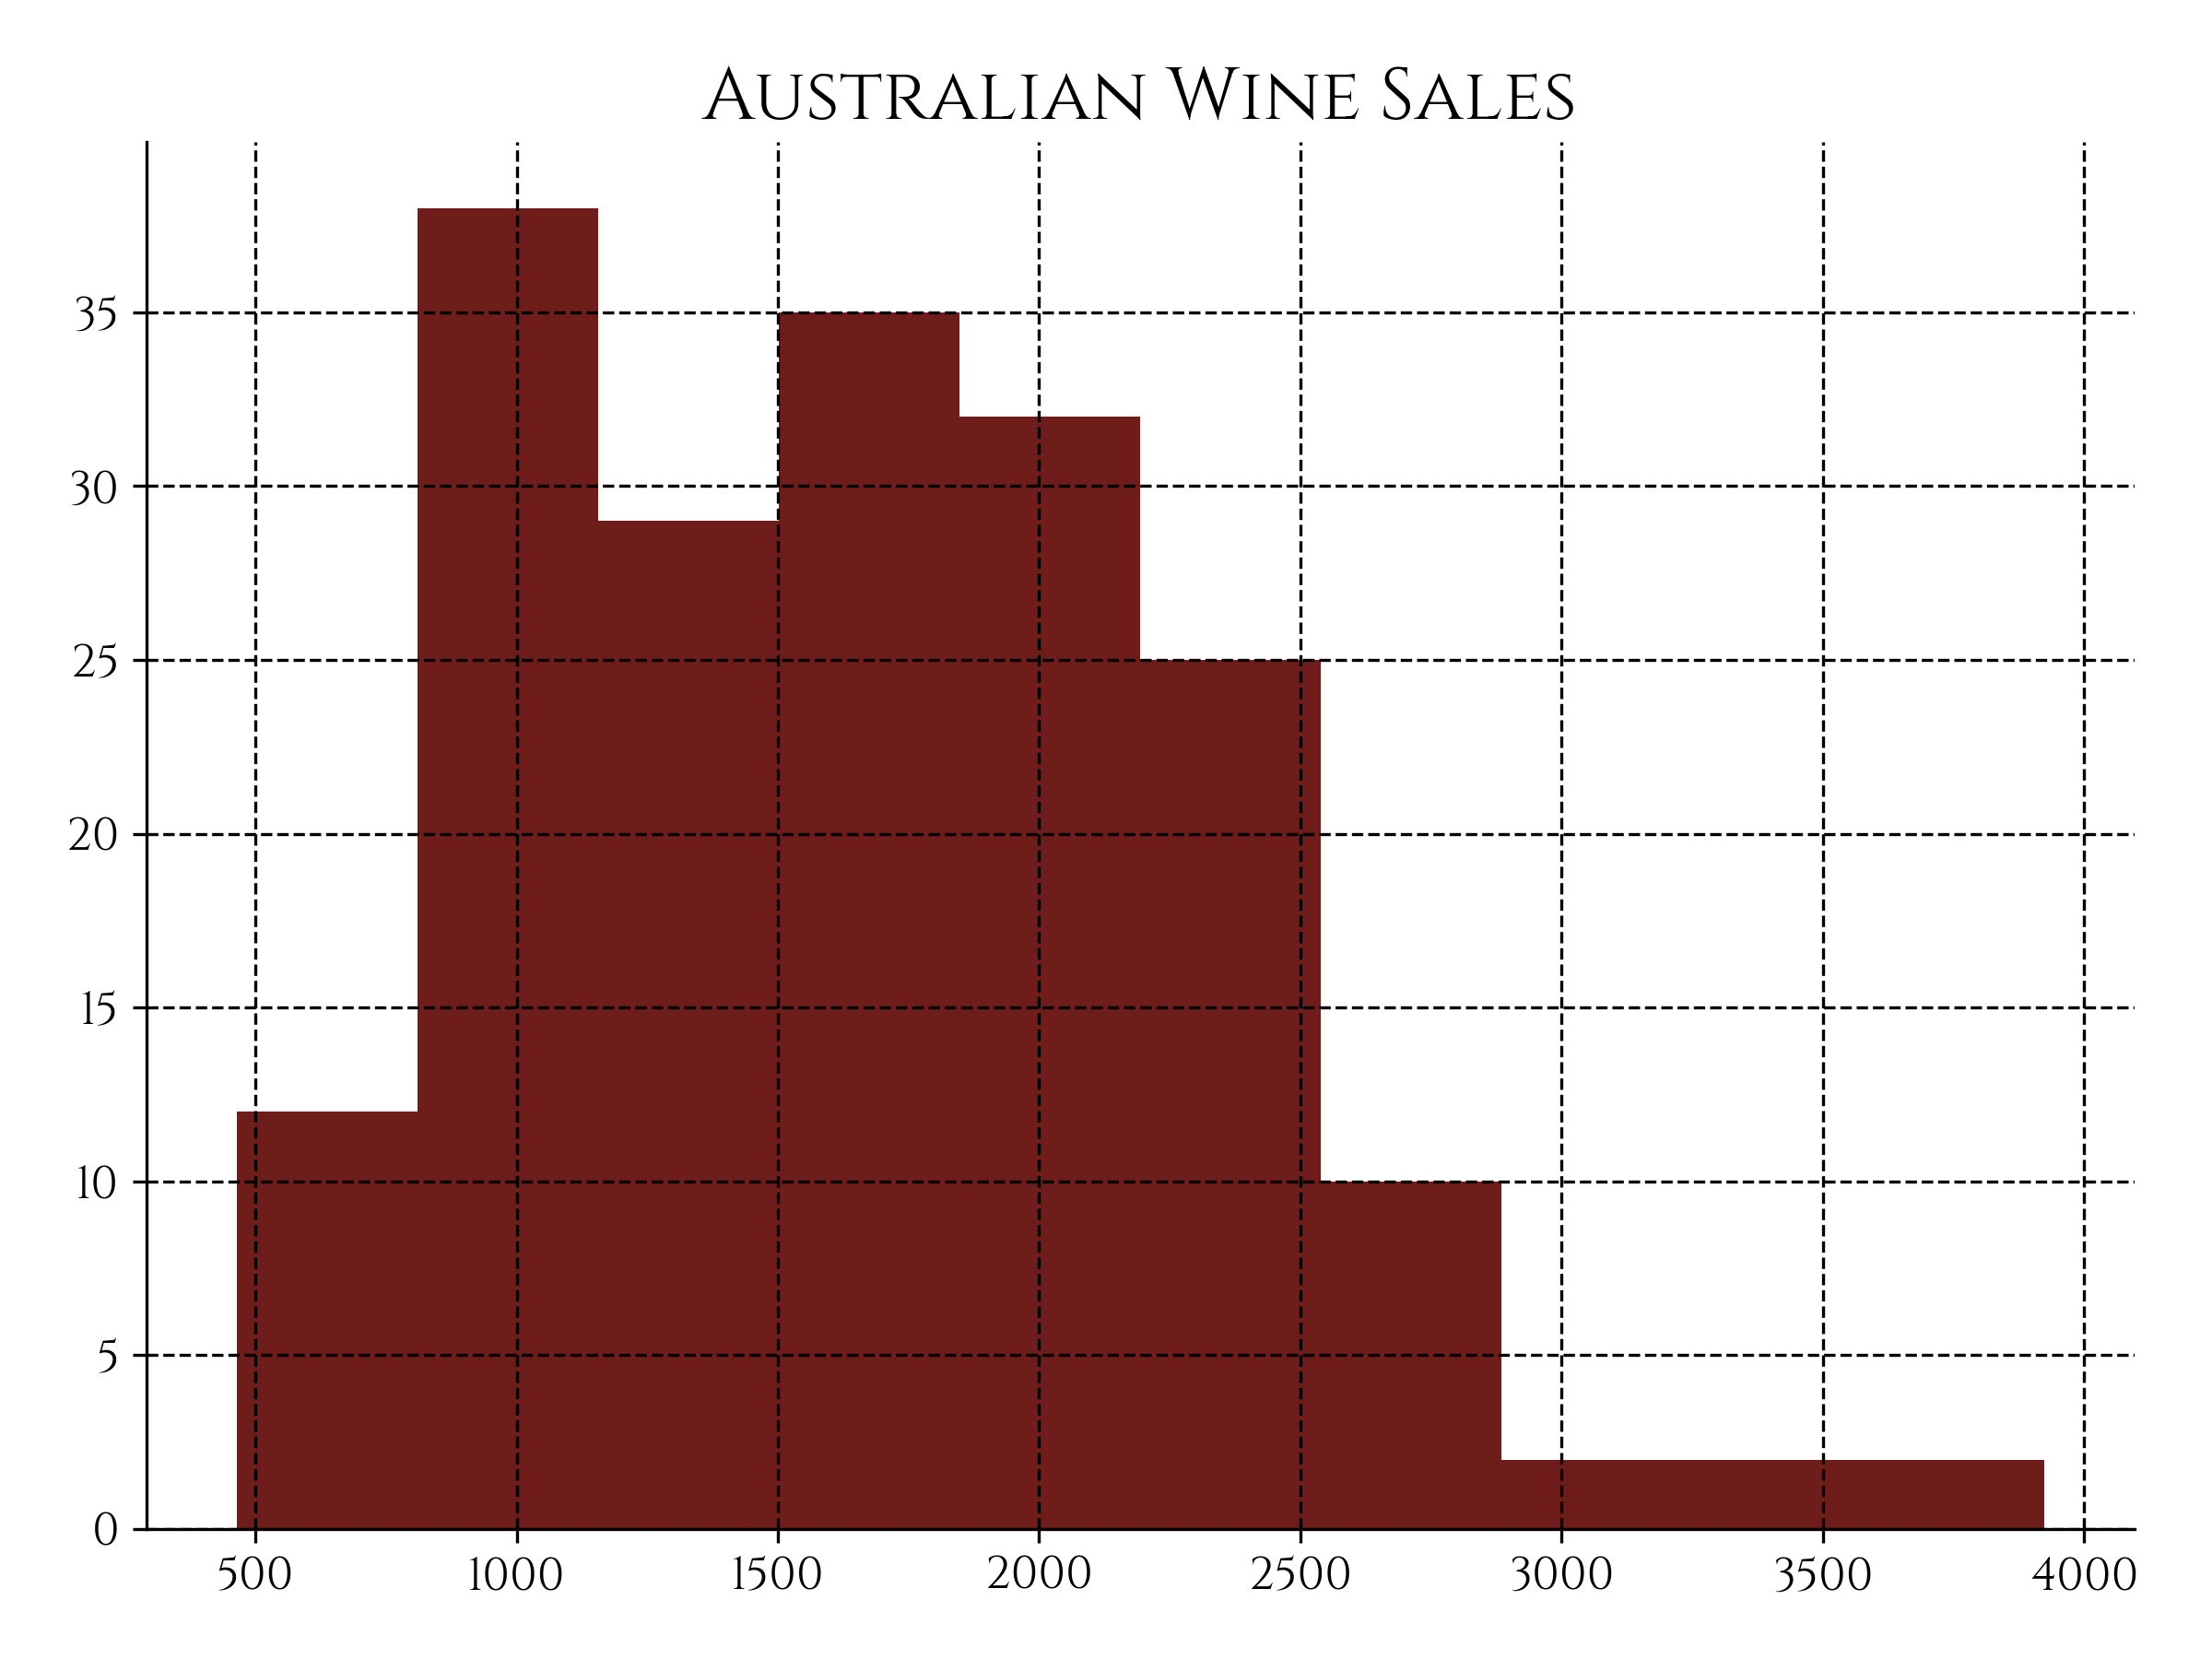
\includegraphics[width=1\textwidth, height=1\textheight, keepaspectratio]{time_series_example_wine_hist}
        \captionof{figure}{Гистограмма месячного объема продаж вина в 
        Австралии. Построено программой по адресу 
        (листинг \ref{lst:time_series_example_wine_hist}).}
        \label{fig:time_series_example_wine_hist}
    \end{minipage}
    \hfill
    \begin{minipage}{0.4\textwidth}
        \centering
        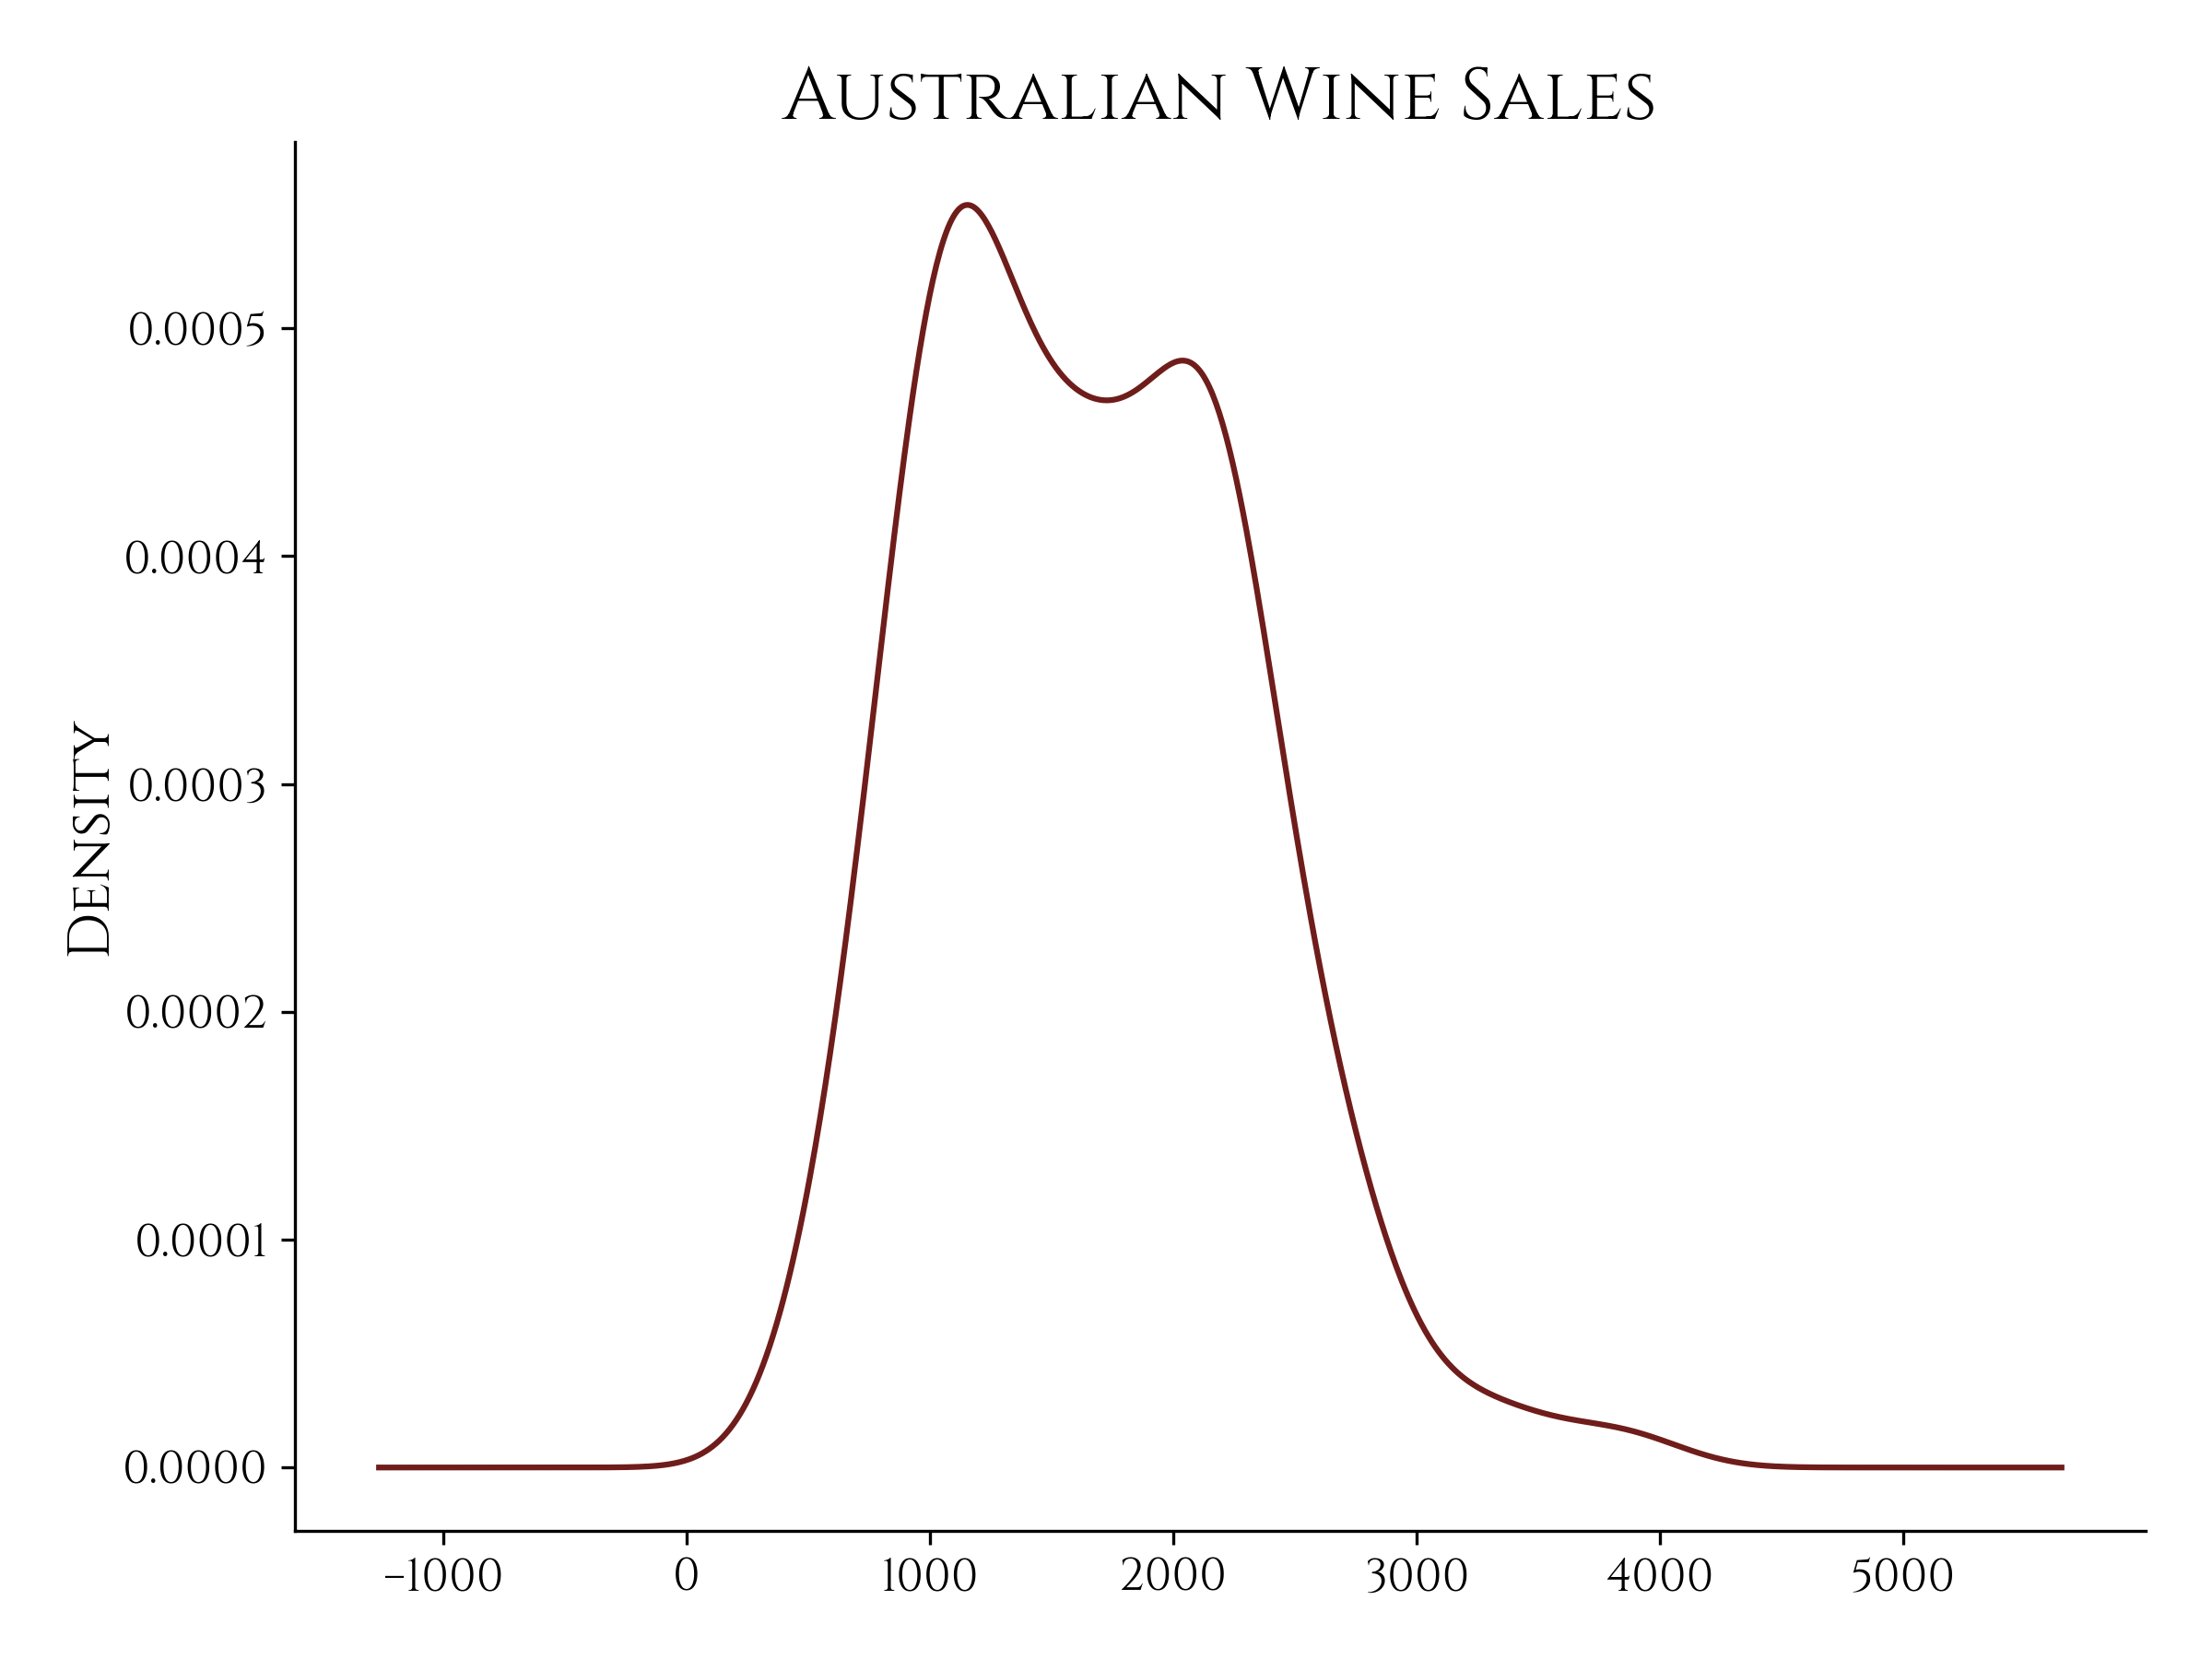
\includegraphics[width=1\textwidth, height=1\textheight, keepaspectratio]{time_series_example_wine_density}
        \captionof{figure}{График плотности месячного объема продаж вина в 
        Австралии. Построено программой по адресу 
        (листинг \ref{lst:time_series_example_wine_density}).}
        \label{fig:time_series_example_wine_density}
    \end{minipage}
\end{center}

\subsubsection{Ящик с усами}

Для интервальной визуализации временных рядов также нередко используют, так 
назваемый, ящик с усами. Данная разновидность графиков основана на 
квартилях набора данных. Так, первый квартиль больше 25\% всех данных и 
меньше других 75\%. Второй квартиль разбивает данные пополам (также известен 
как медиана). Третий - больше 75\% всех данных и меньше оставшихся 25\%. Первый 
и третий квартили как раз образуют стенки ящика. А
\guillemotleft усы\guillemotright {}, в свою очередь, обычно
захватывают все оставшиеся данные, не считая 
выбросы (в разных источниках бывает по разному). Рассмотрим данный вид диаграмм:

\begin{figure}[h!]
    \centering
    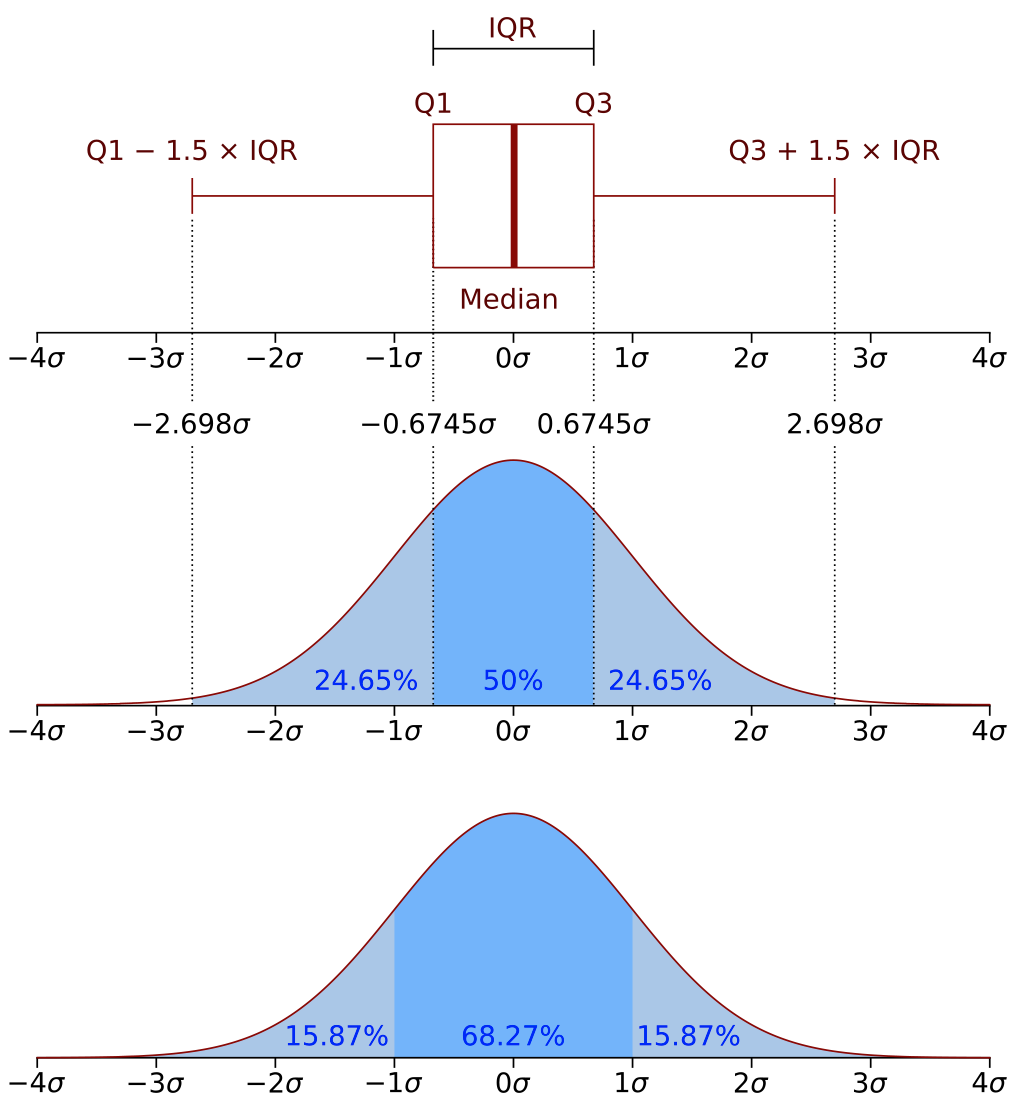
\includegraphics[width=0.45\textwidth, height=0.45\textheight, keepaspectratio]{boxplot_explanation}
    \captionof{figure}{ Ящик с усами и функция плотности вероятности (pdf) 
    нормального распределения $N(0, \sigma^2)$ \cite{wiki_boxplot}.}
    \label{fig:boxplot_explanation}
\end{figure}

\newpage

\begin{figure}[h!]
    \centering
    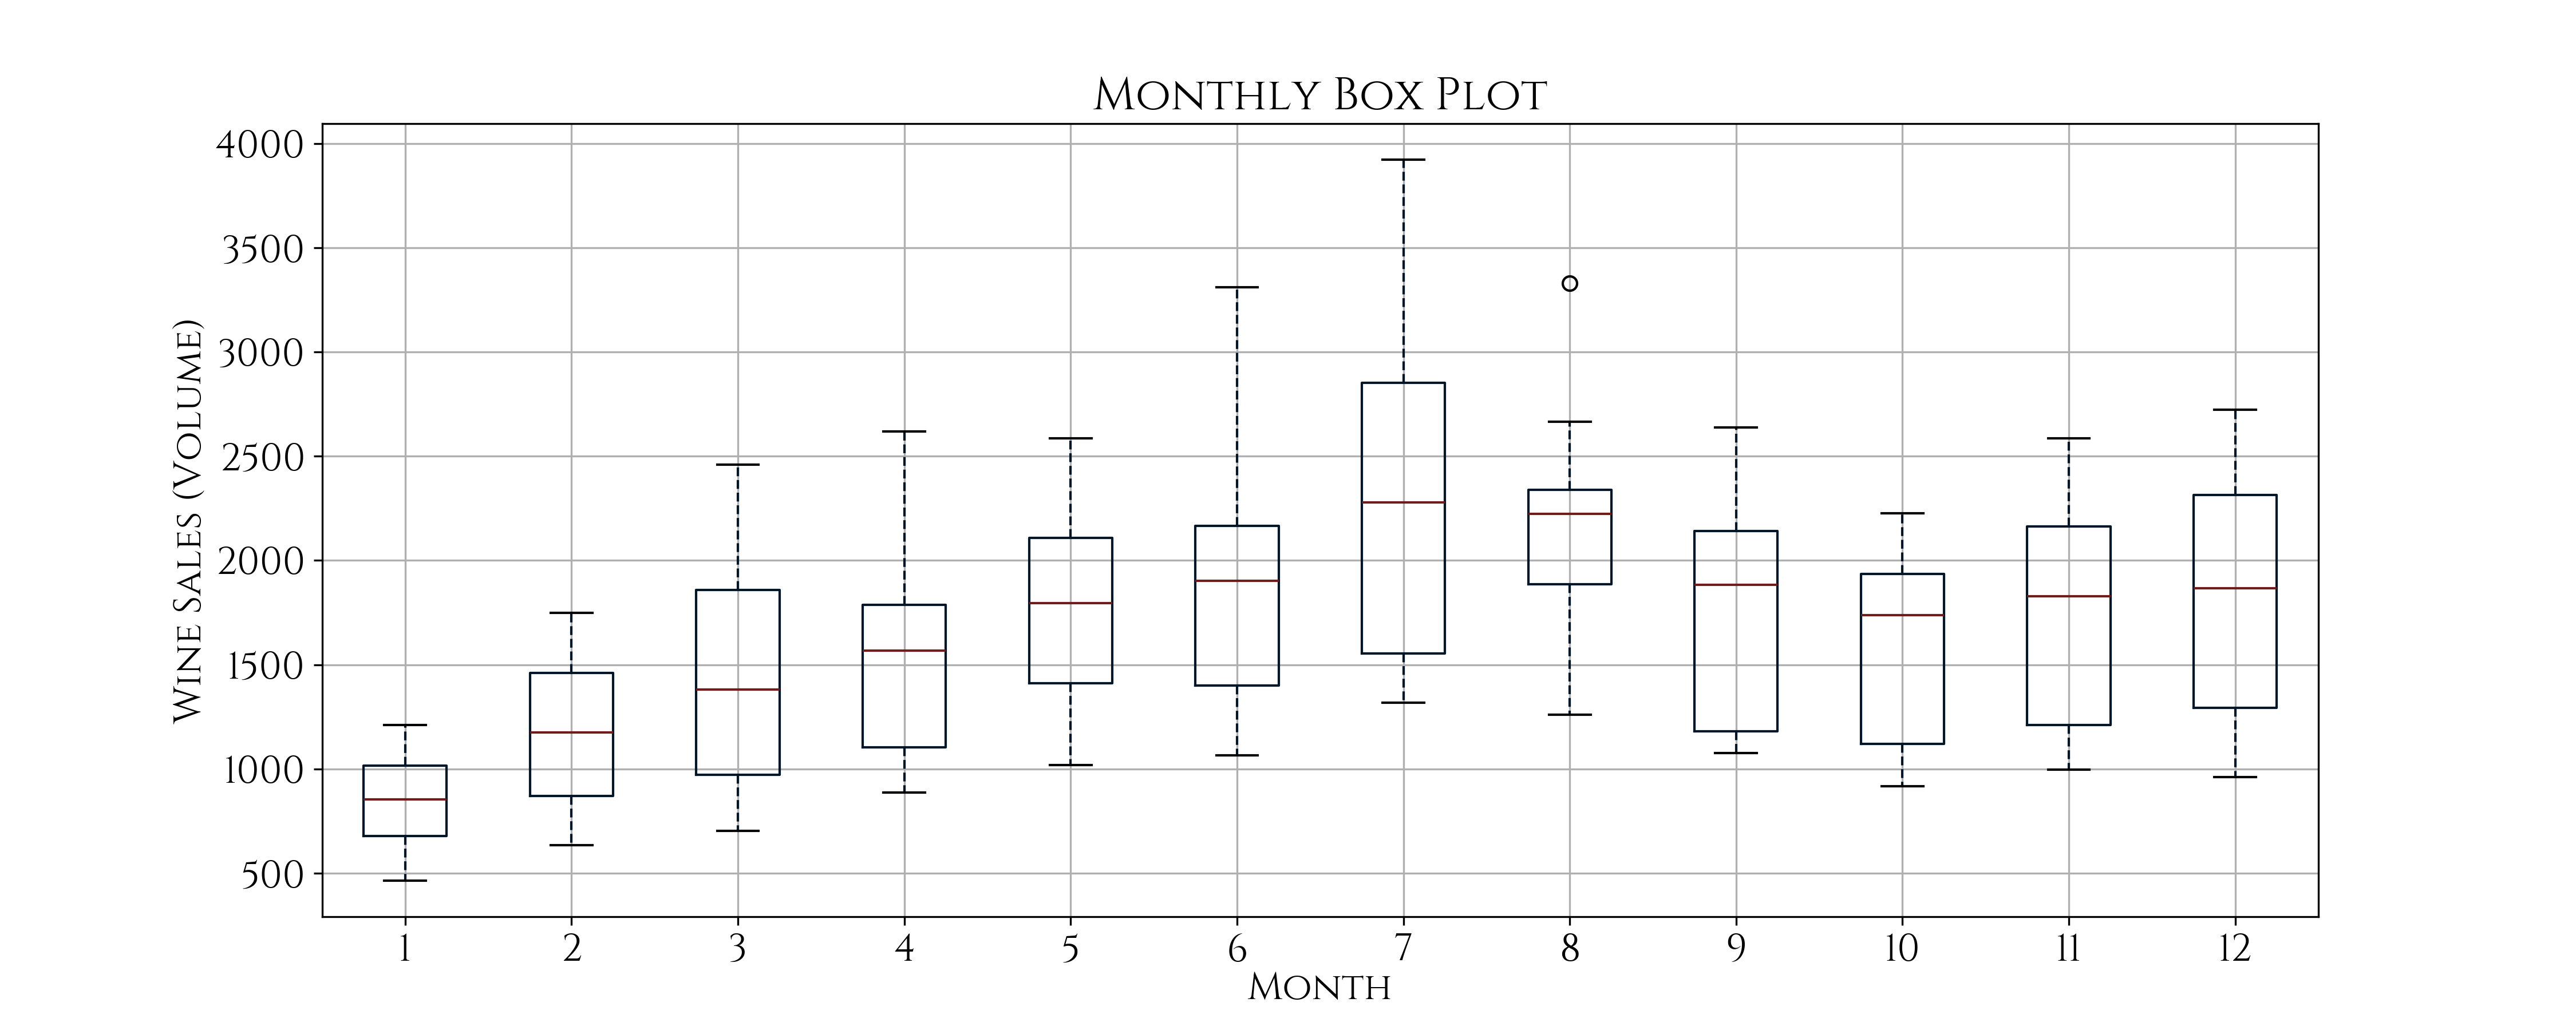
\includegraphics[width=1\textwidth, height=1\textheight, keepaspectratio]{time_series_example_wine_boxplot}
    \captionof{figure}{Распределения продаж красного вина в Австралии по месяцам в период с 1980 по 1996 года. 
    Построено программой по адресу 
    (листинг \ref{lst:time_series_example_wine_boxplot}).}
    \label{fig:time_series_example_wine_boxplot}
\end{figure}

\subsubsection{График задержек}
Графиком задержек (Lag Plot) называется особый вид диаграммы рассеяния (scatter plot), 
на которой по одной из ее осей откладывается значение временного ряда в момент времени 
$t$, а по другой - значение в момент времени $t + l$, где $l$ - значение лага.

\begin{center}
    \begin{minipage}{0.45\textwidth}
        \centering
        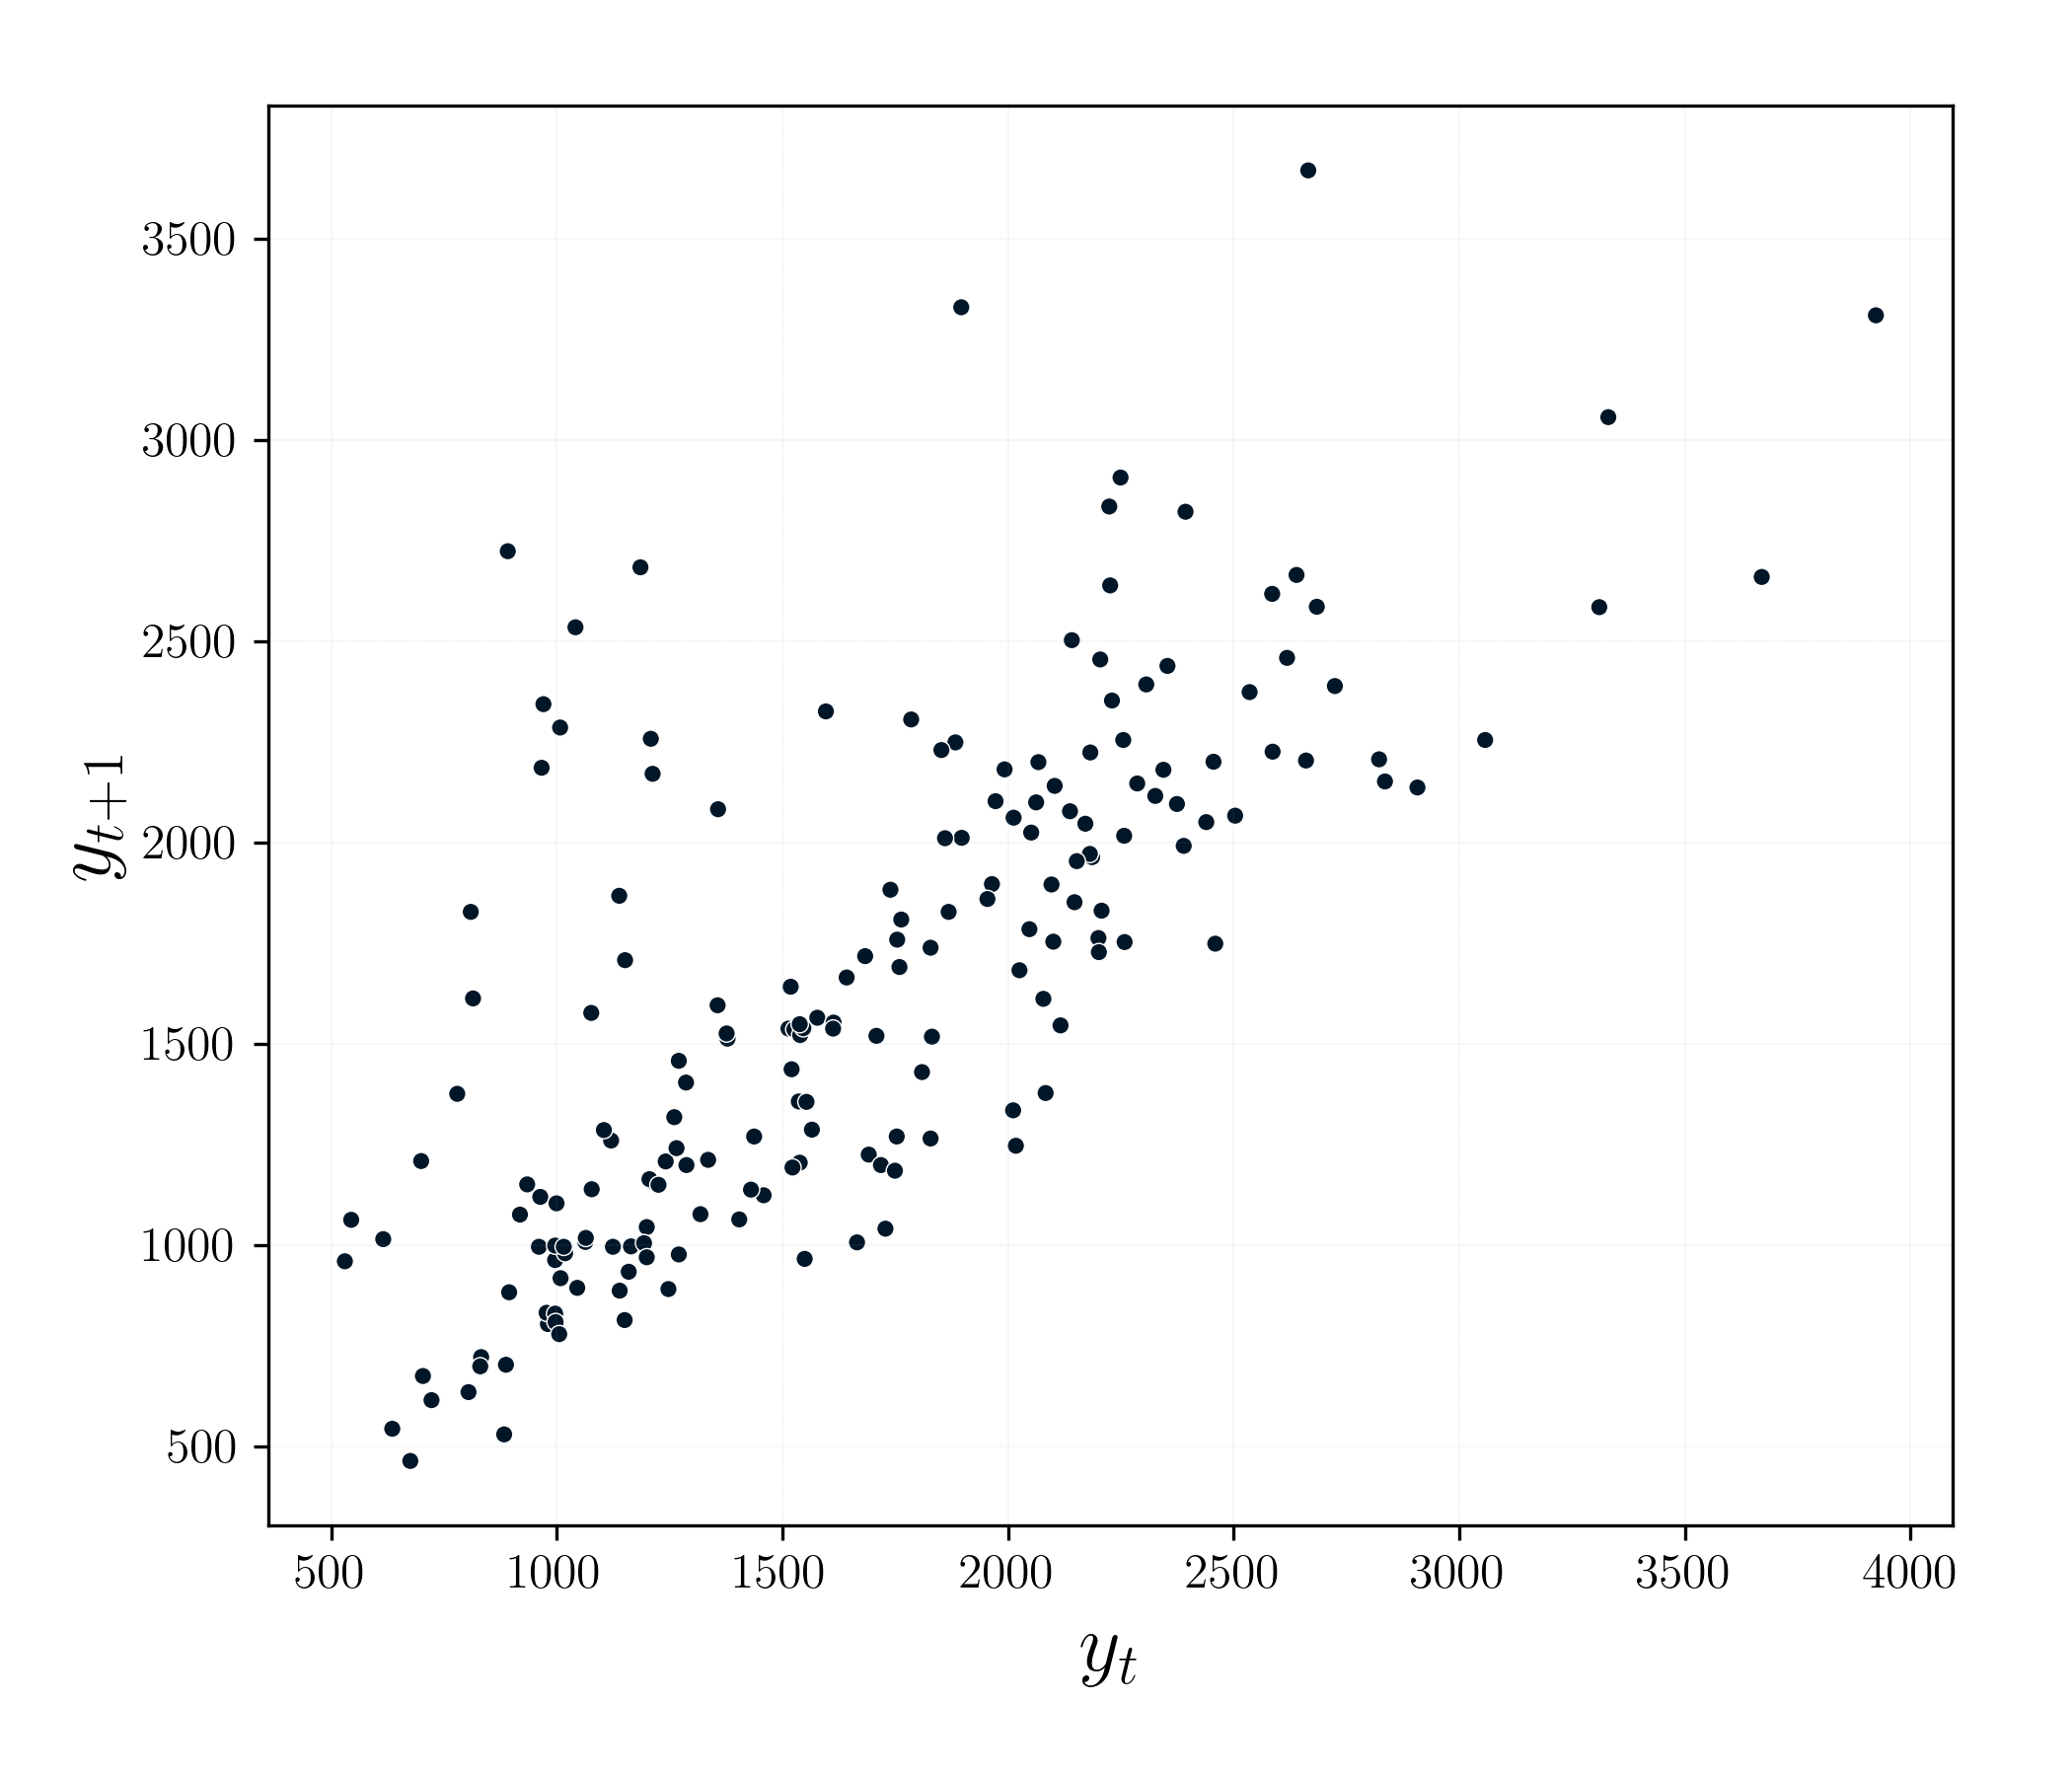
\includegraphics[width=1\textwidth, height=1\textheight, keepaspectratio]{australia_wine_lag_plot}
        \captionof{figure}{Связь между значениями объёма продаж красного вина в соседние месяцы, 
        по горизонтали отложен объём продаж в месяц t, по вертикали — в следующий месяц, 
        t + 1. Построено программой по адресу 
        (листинг \ref{lst:time_series_lag_plot_wine}).}
        \label{fig:lag_plot_wine}
    \end{minipage}
    \hfill
    \begin{minipage}{0.45\textwidth}
        \centering
        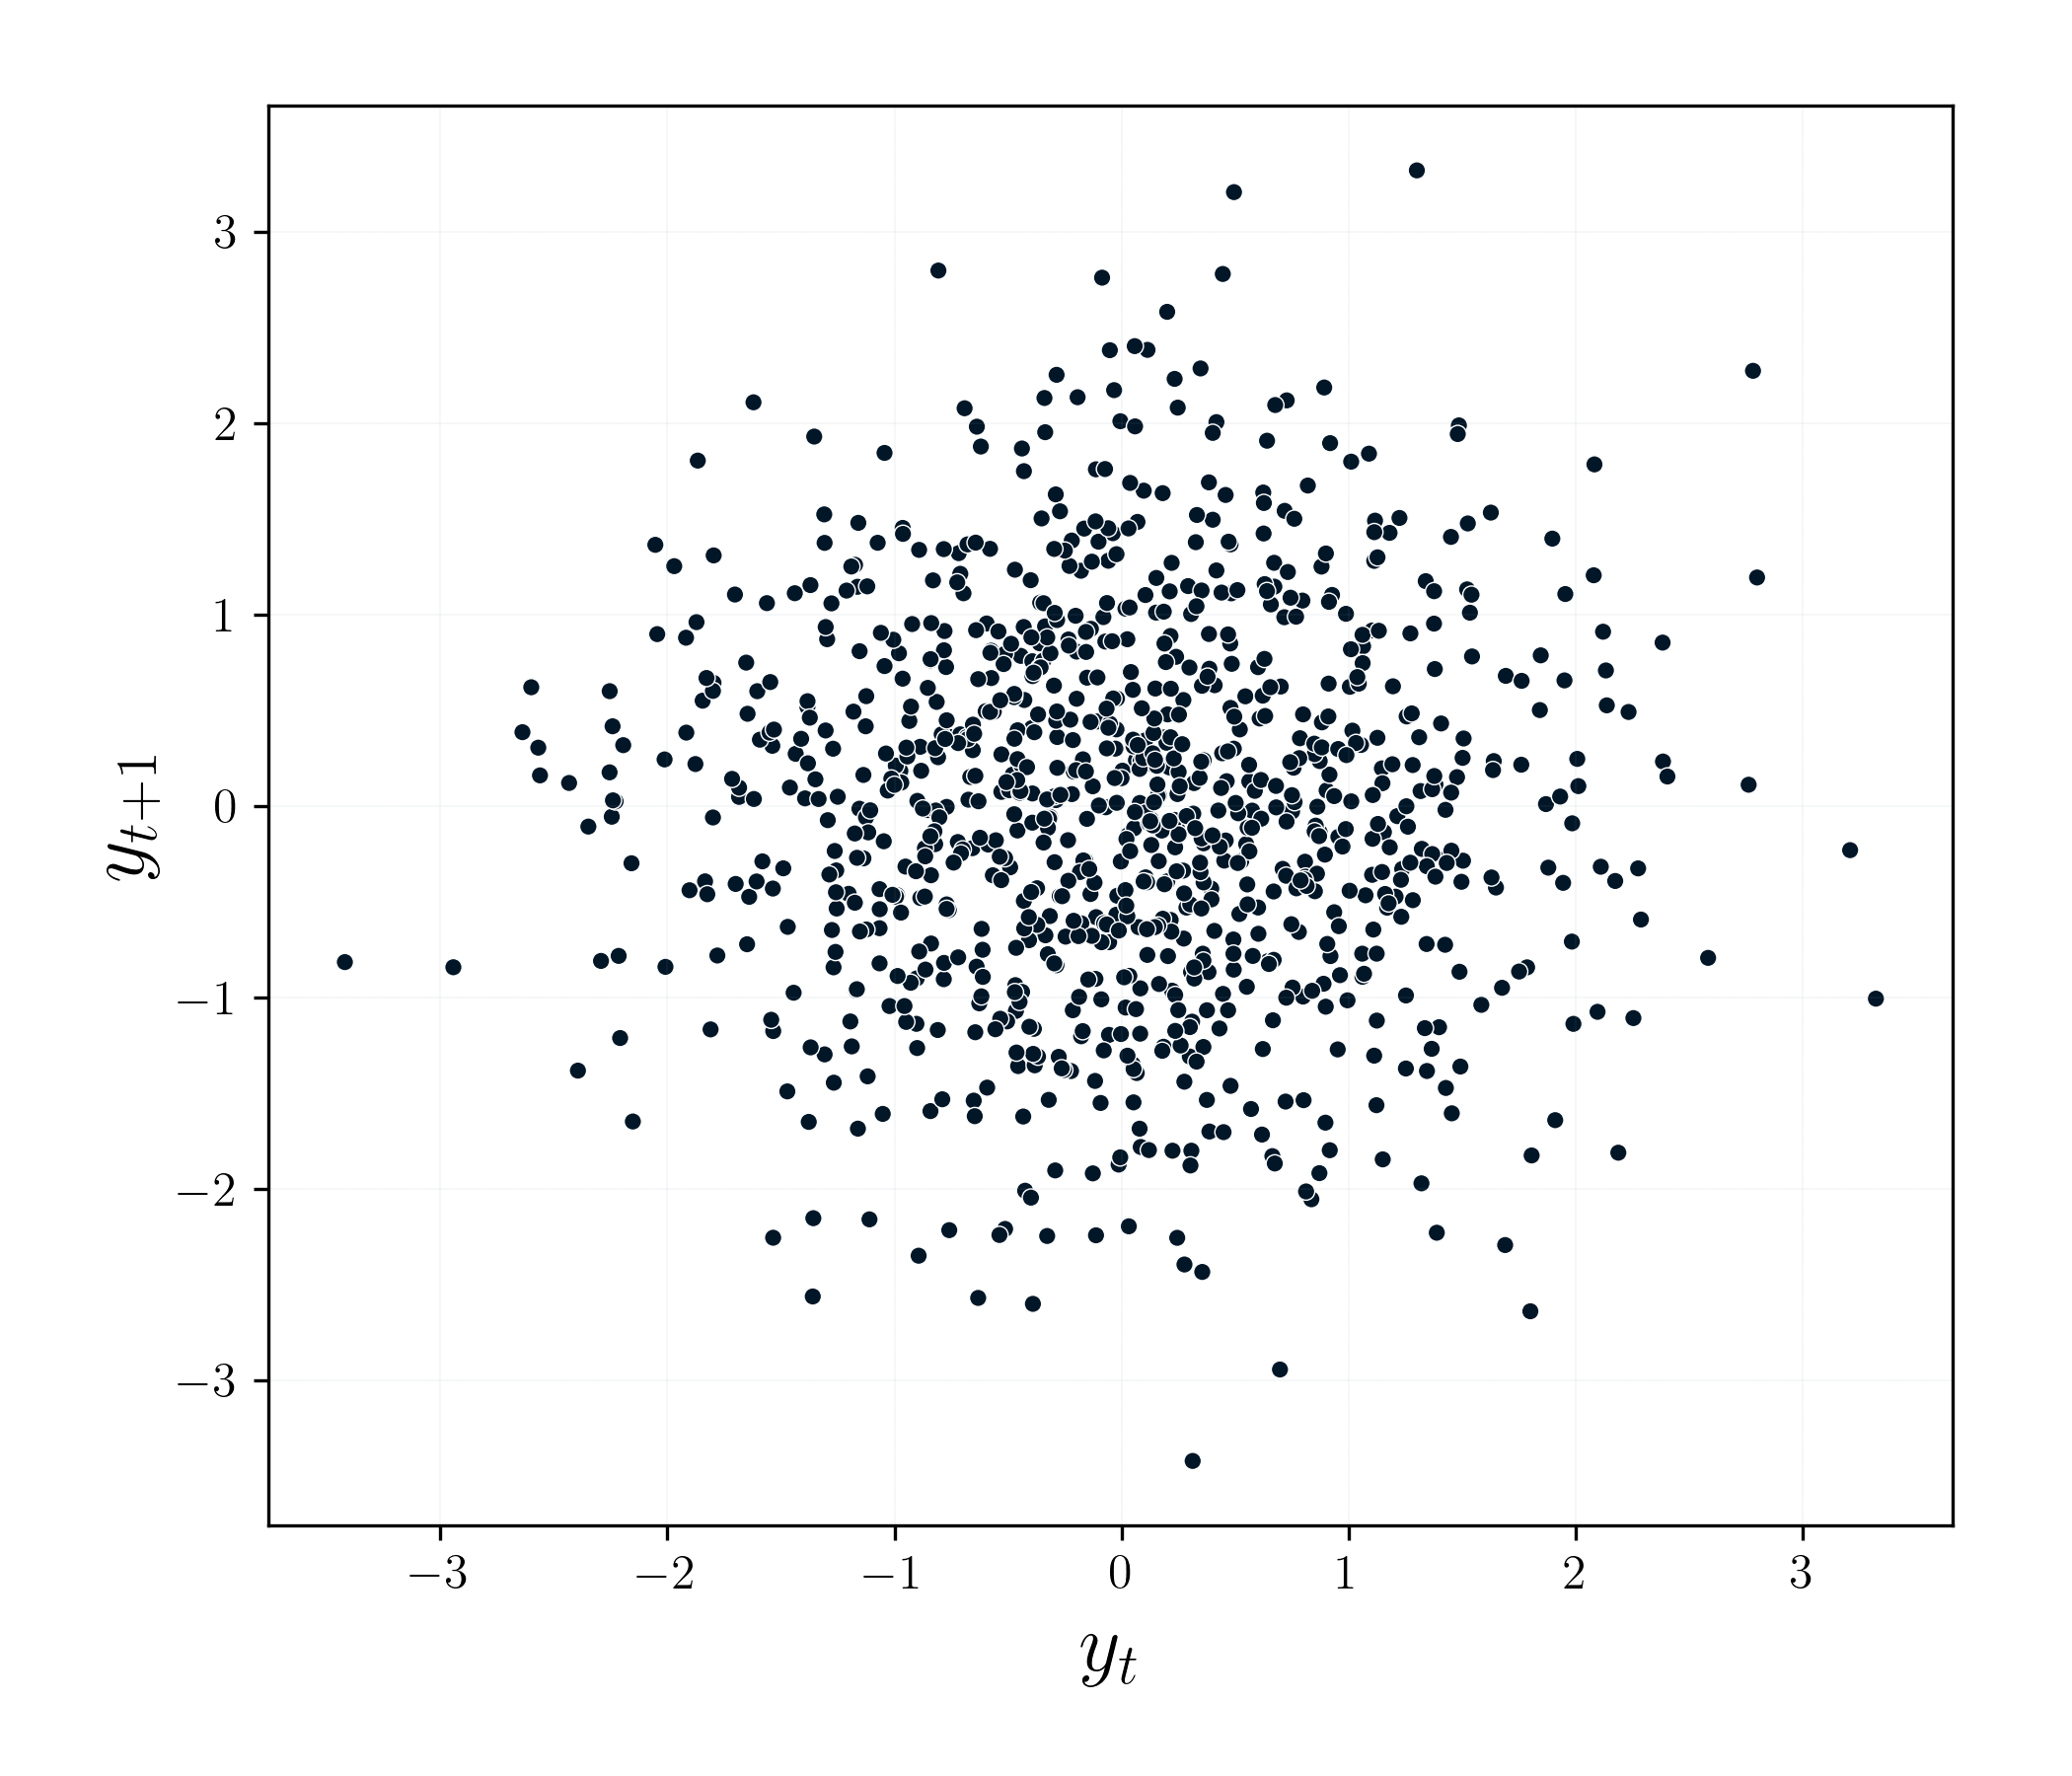
\includegraphics[width=1\textwidth, height=1\textheight, keepaspectratio]{random_series_lag_plot}
        \captionof{figure}{График задержек случайных величин, взятых из нормального 
        распределения с лагом $l = 1$. Построено программой по адресу 
        (листинг \ref{lst:time_series_lag_plot_random}).}
        \label{fig:lag_plot_random}
    \end{minipage}
\end{center}

График задержек помогает понять являются ли значения во временном ряду случайными. Если 
данные случайны, то на графике мы не увидим никакой определенной структуры. Однако 
если же данные не случайны, то на графике задержек можно будет увидеть ярко 
выраженную форму. 

Например на рисунке \ref{fig:lag_plot_wine} видно, что большая часть точек 
сгруппирована вокруг главной диагонали, что говорит о схожести продаж в соседние месяцы. 
В свою очередь на рисунке \ref{fig:lag_plot_random} нет никакой ярко выраженной 
структуры, что логично, так как это просто белый шум. \\

\subsubsection{Матрица корреляций}

Еще одним широко распространенным методом графического анализа автокорреляции 
временного ряда является матрица корреляций (корреляционная матрица). Она отображает в 
себе корреляцию между всеми возможными заданными парами значений.

Рассмотрим матрицу корреляций на примере еженедельного общего объема продаж авокадо 
за 3 года (рис. \ref{fig:time_series_avocado}).

\begin{figure}[h!]
    \centering
    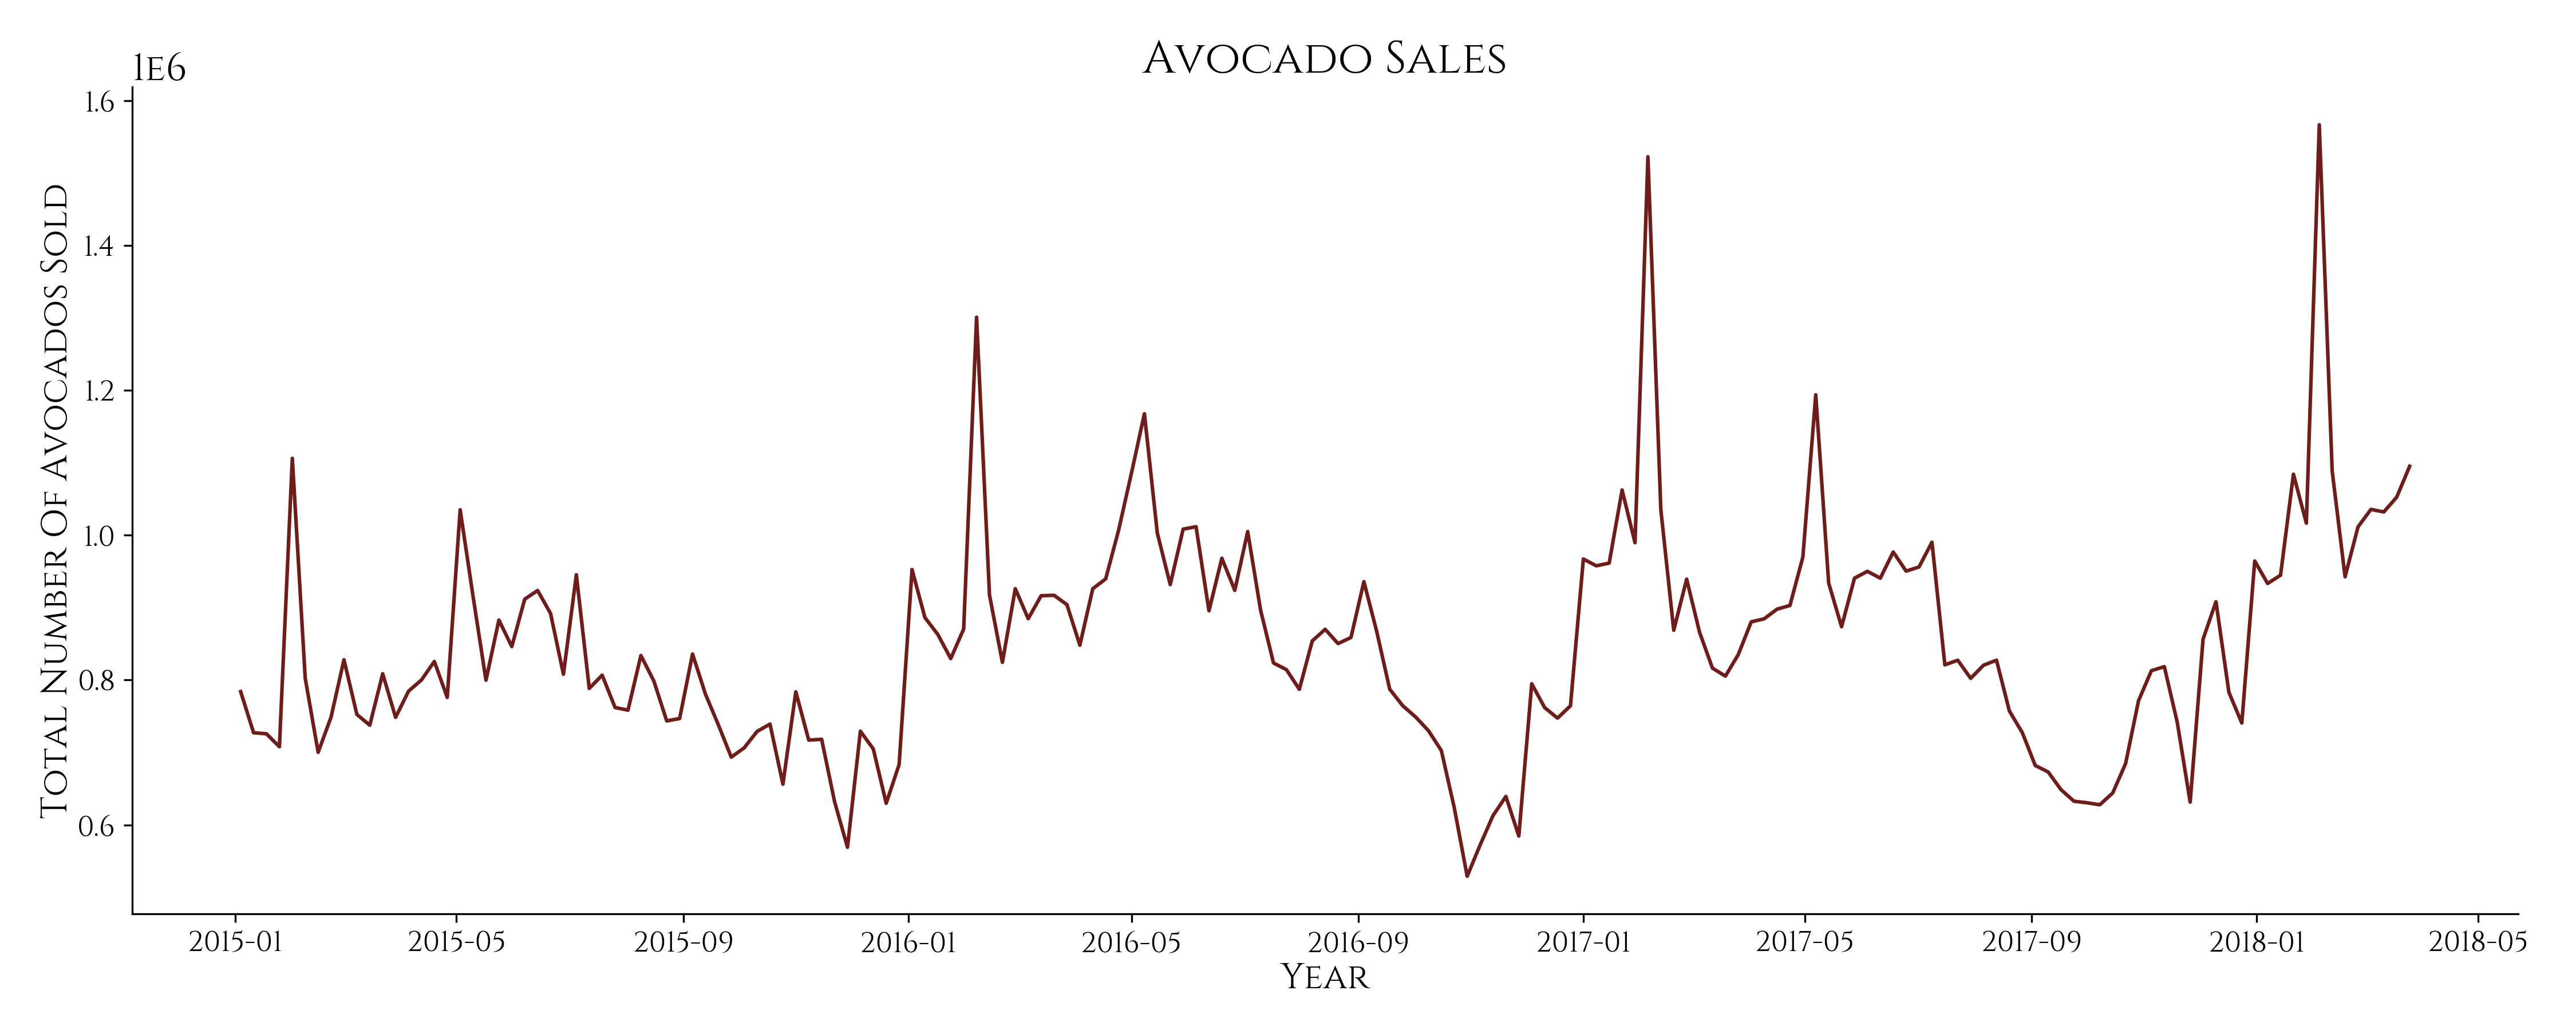
\includegraphics[width=1\textwidth, height=1\textheight, keepaspectratio]{time_series_example_avocado}
    \caption{Еженедельный объём продаж авокадо. Построено программой по адресу 
    (листинг \ref{lst:time_series_example_avocado}).}
    \label{fig:time_series_avocado}
\end{figure}

\begin{figure}[h!]
    \centering
    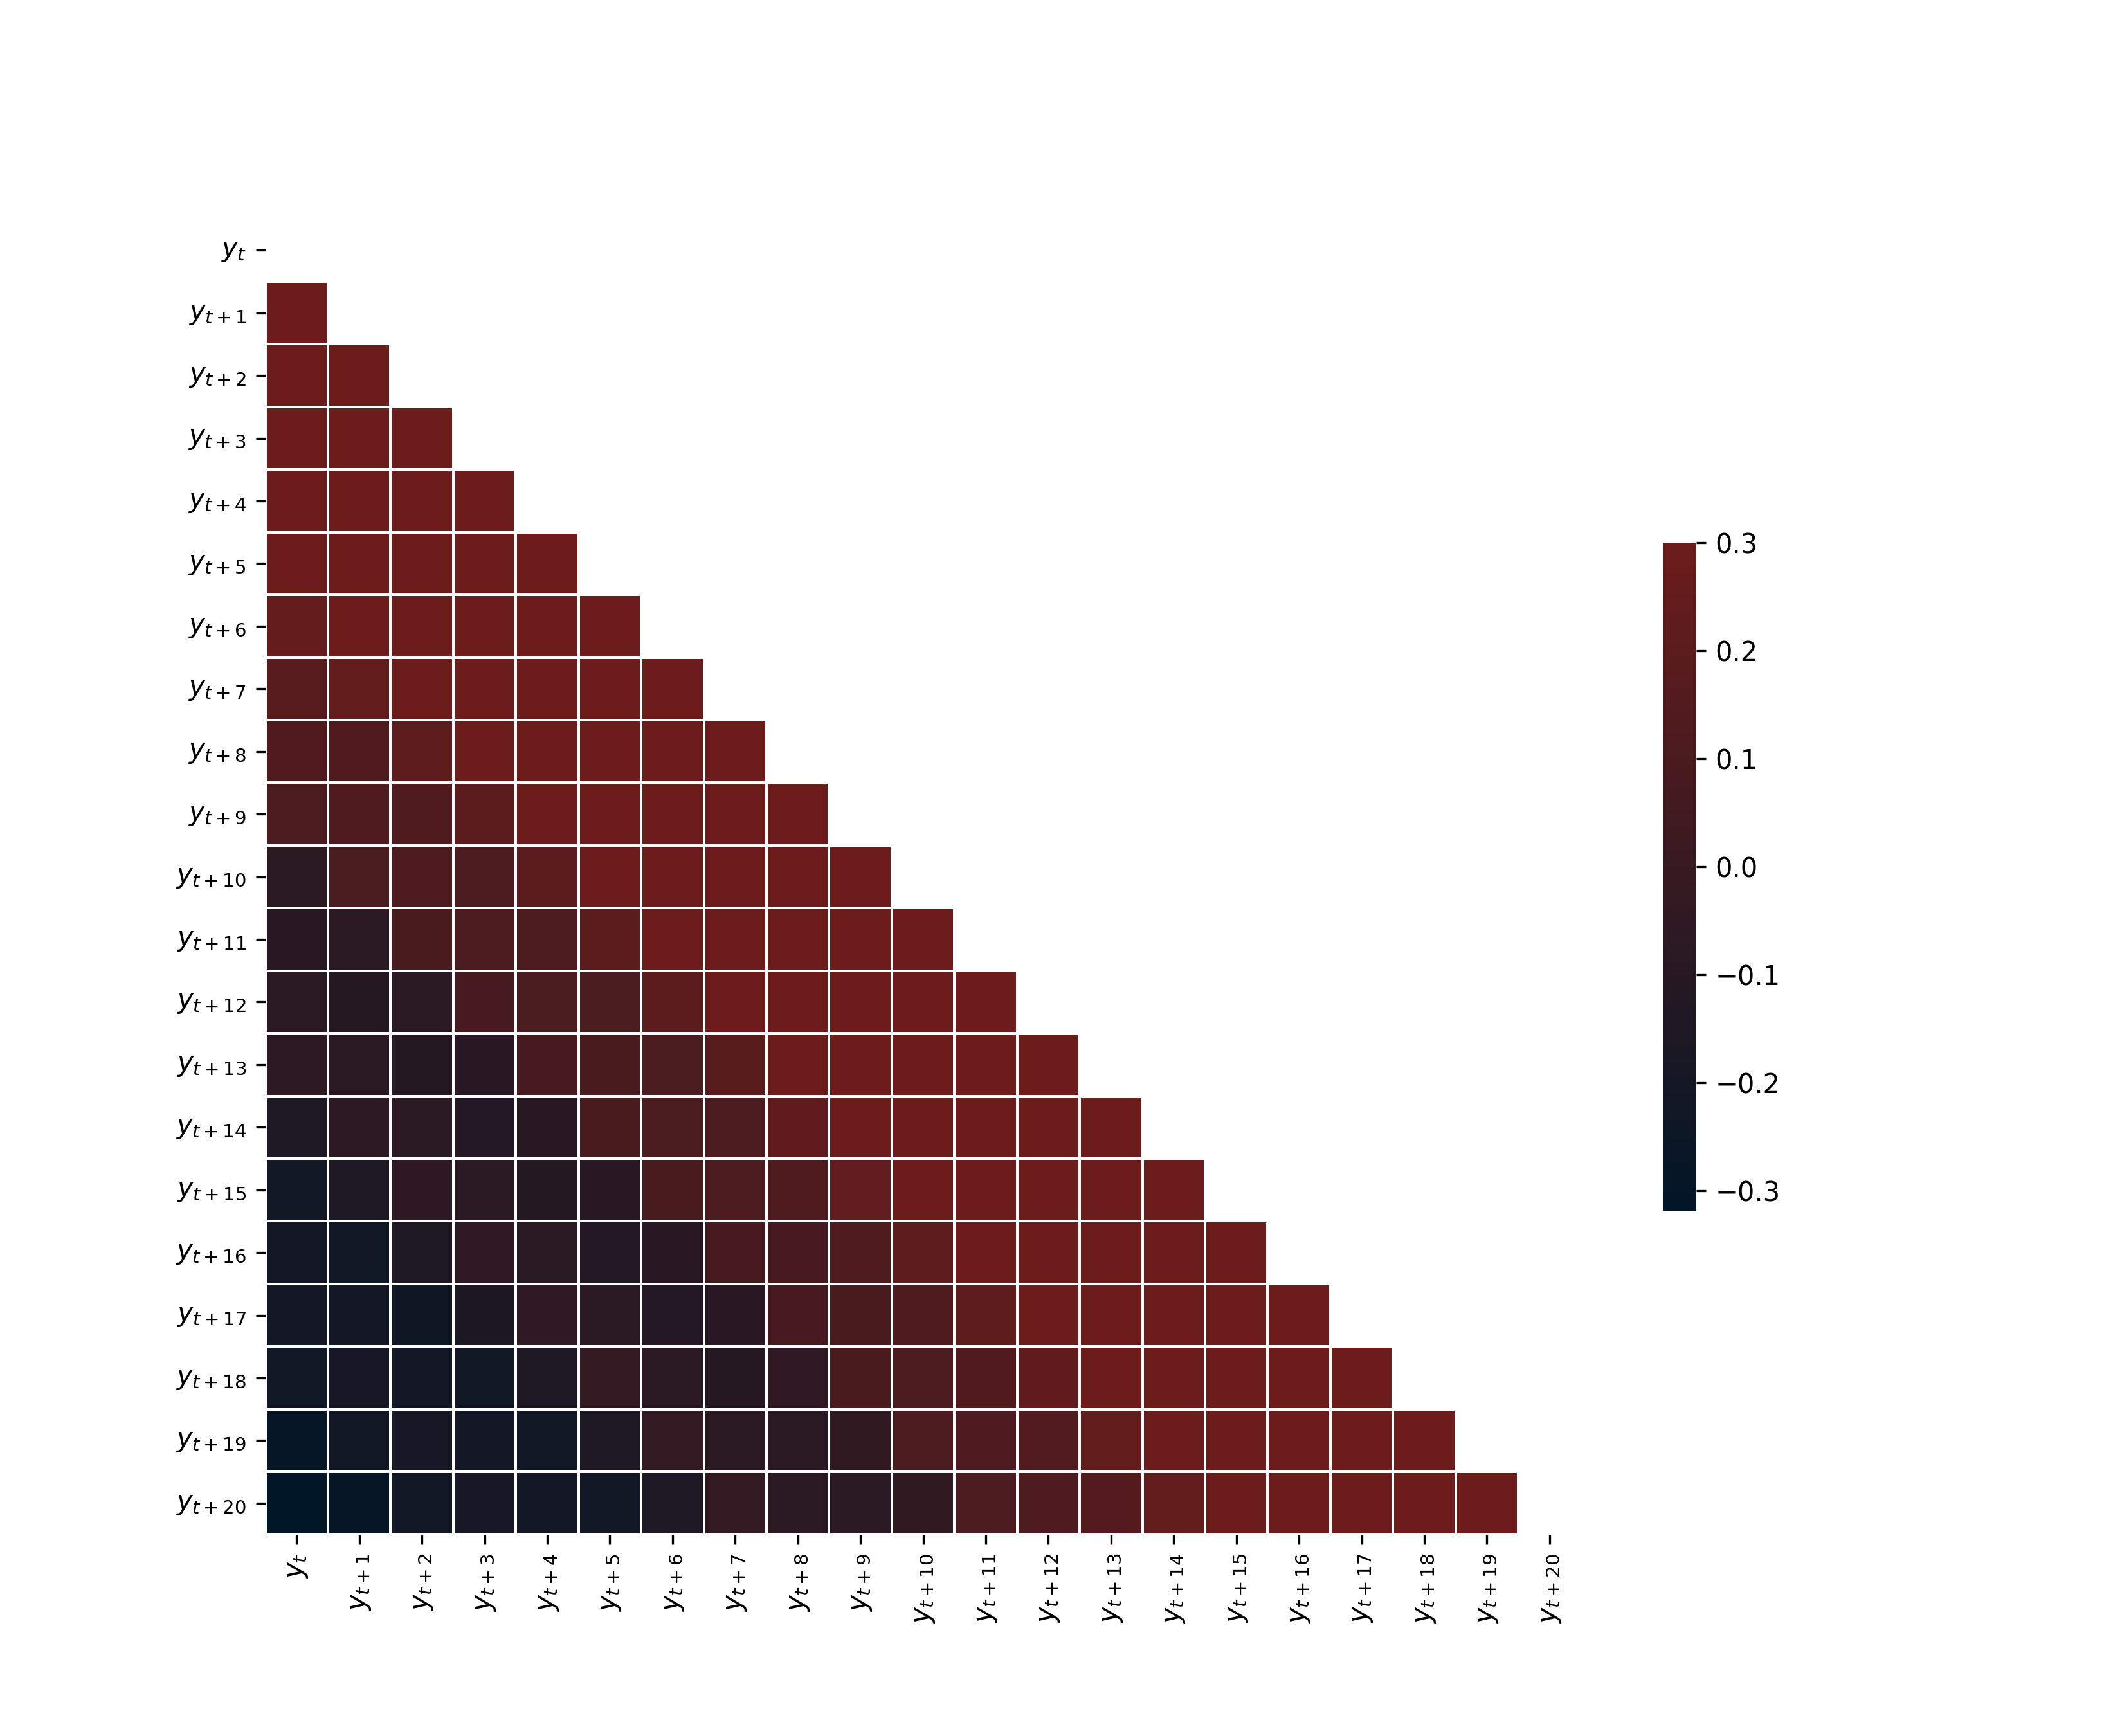
\includegraphics[width=1\textwidth, height=1\textheight, keepaspectratio]{correlation_matrix_avocado}
    \caption{Диагональная корреляционная матрица объема продаж авокадо. Построено 
    программой по адресу (листинг \ref{lst:correlation_matrix_avocado}).}
    \label{fig:correlation_matrix_avocado}
\end{figure}

\newpage

На рисунке \ref{fig:correlation_matrix_avocado} видно, что данные тем сильнее 
скоррелированны, чем ближе они находятся. Так например значения в соседних точках 
временного ряда $y_t$ и $y_{t+1}$ имеют корреляцию равную $0.3$, а $y_t$ и $y_{t+20}$, 
в свою очередь: $-0.3$.

\subsubsection{Автокорреляционная функция}

График автокорреляции временного ряда от лага называется автокорреляционной 
функцией (ACF). Такой график также часто называют коррелограммой. По оси ординат на 
нём откладывается автокорреляция, а по оси абсцисс — размер лага $l$.

\begin{figure}[h!]
    \centering
    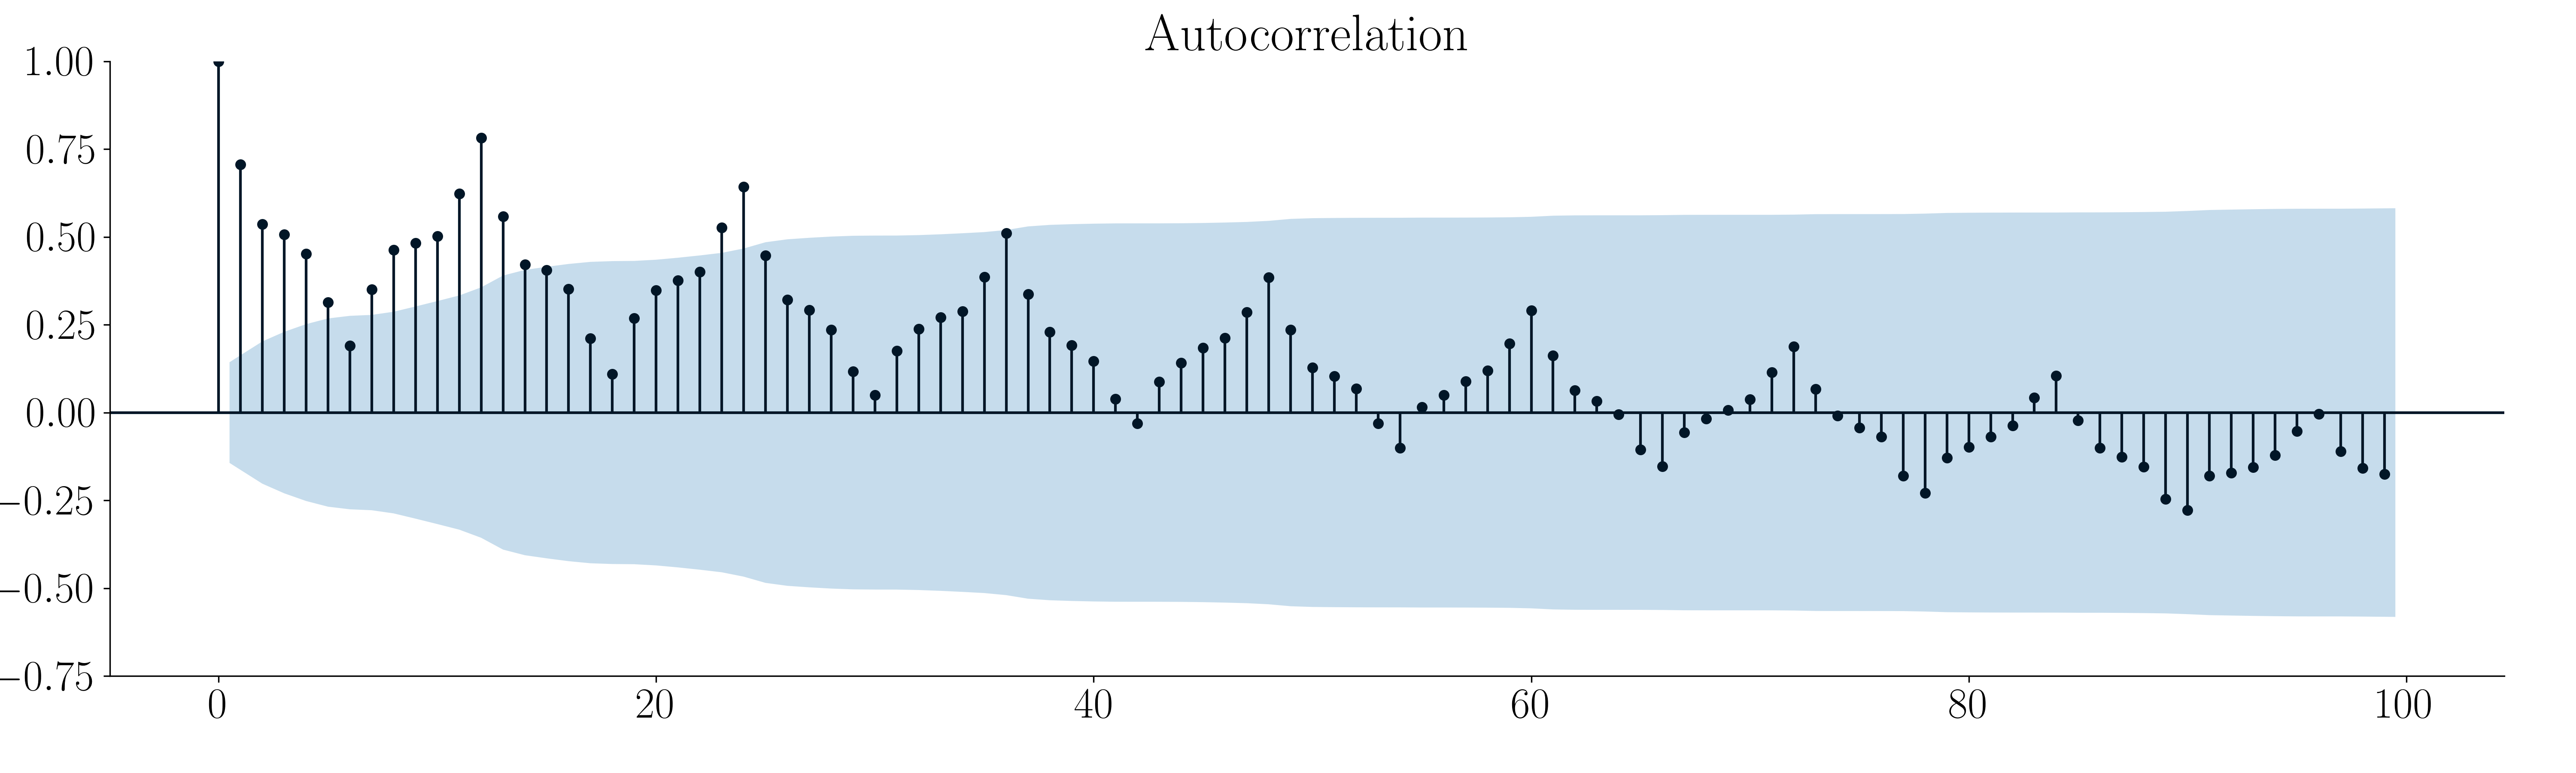
\includegraphics[width=1\textwidth, height=1\textheight, keepaspectratio]{acf_wine}
    \caption{Коррелограмма для объёма продаж красного вина в Австралии. Построено 
    программой по адресу (листинг \ref{lst:acf_wine}).}
    \label{fig:acf_wine}
\end{figure}

На рисунке \ref{fig:acf_wine} показан пример коррелограммы для исследуемых 
ранее данных о месячных продажах красного вина в Австралии 
(рисунок \ref{fig:time_series_wine}). На графике видно, что автокорреляция принимает 
большие значения в лагах, кратных сезонному периоду. Такой вид коррелограммы 
типичен для данных с выраженной сезонностью.

Стоит отметить, что автокорреляция может начать колебаться вокруг горизонтальной оси, 
соответствующей её нулевому значению, как это и произошло на рисунке \ref{fig:acf_wine}, 
а также, что автокорреляция в точке с лагом $l = 0$ всегда равна единице, 
так как в ней вычисляется корреляция значения ряда с самим собой.

Также на рисунке \ref{fig:acf_wine} изображён синий коридор вокруг горизонтальной оси. 
Это коридор значимости отличия корреляции от нуля. Фактически, все автокорреляции, 
которые изображены вне этого коридора, значимо отличаются от нуля.

\subsection{Стационарность}

Если $\left\{y_t\right\}$ - стационарный временной ряд, то 
для любого $s$, распределение $(y_t, \dots, y_{t+s})$ не зависит 
от $t$ \cite{Forecasting_Hyndman}. 

Таким образом, временные ряды с выраженным трендом или сезонностью не являются стационарными.
С другой стороны, белый шум, например, является стационарным - неважно в какой момент времени 
мы его рассмотрим, он будет выглядеть одинаково.

Иногда бывает затруднительно определить, является ли ряд стационарным. Временные ряды с 
непереодическими циклами (но без тренда или сезонности), например, не обязательно нестационарны, поскольку 
нельзя заранее предсказать положение максимумов и минимумов ряда.

\begin{figure}[h!]
    \centering
    % First Row
    \subcaptionbox{листинг \ref{lst:time_series_example_avocado} \label{fig:time_series_example_avocado_small}}[0.3\textwidth]{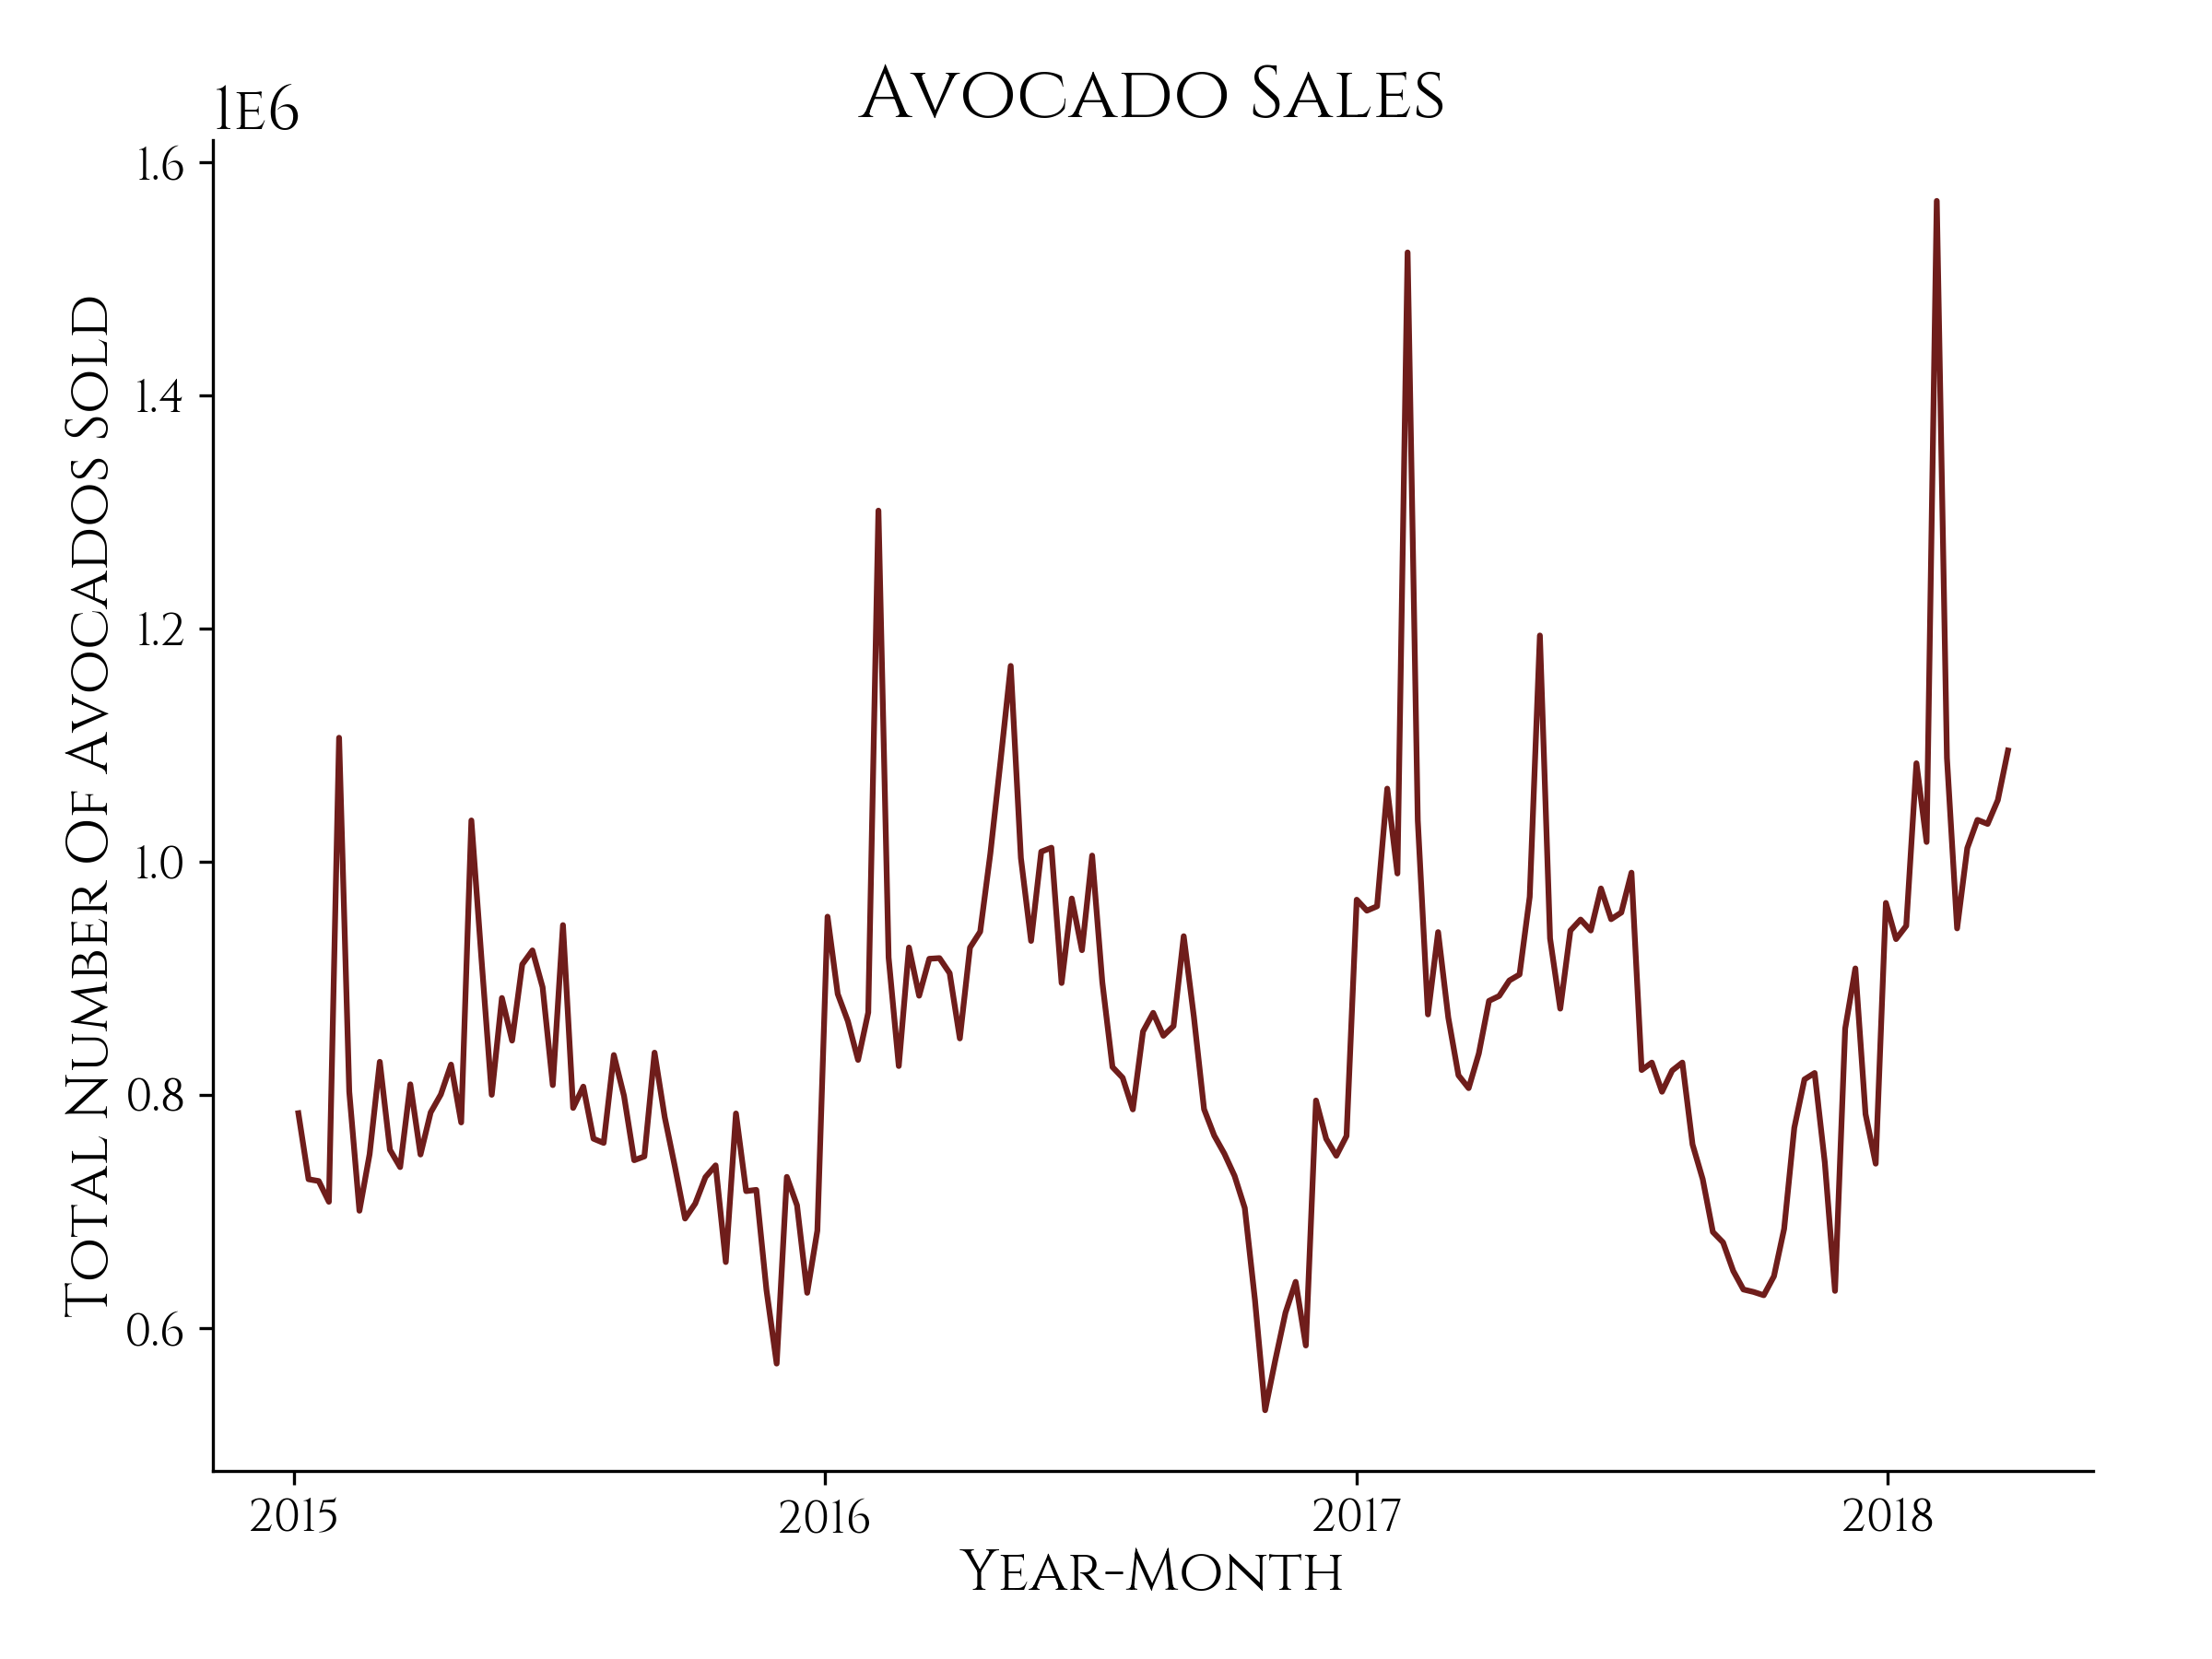
\includegraphics[width=0.3\textwidth, keepaspectratio]{time_series_example_avocado_small}}
    \hfill
    \subcaptionbox{листинг \ref{lst:time_series_example_random_small} \label{fig:time_series_example_random_small}}[0.3\textwidth]{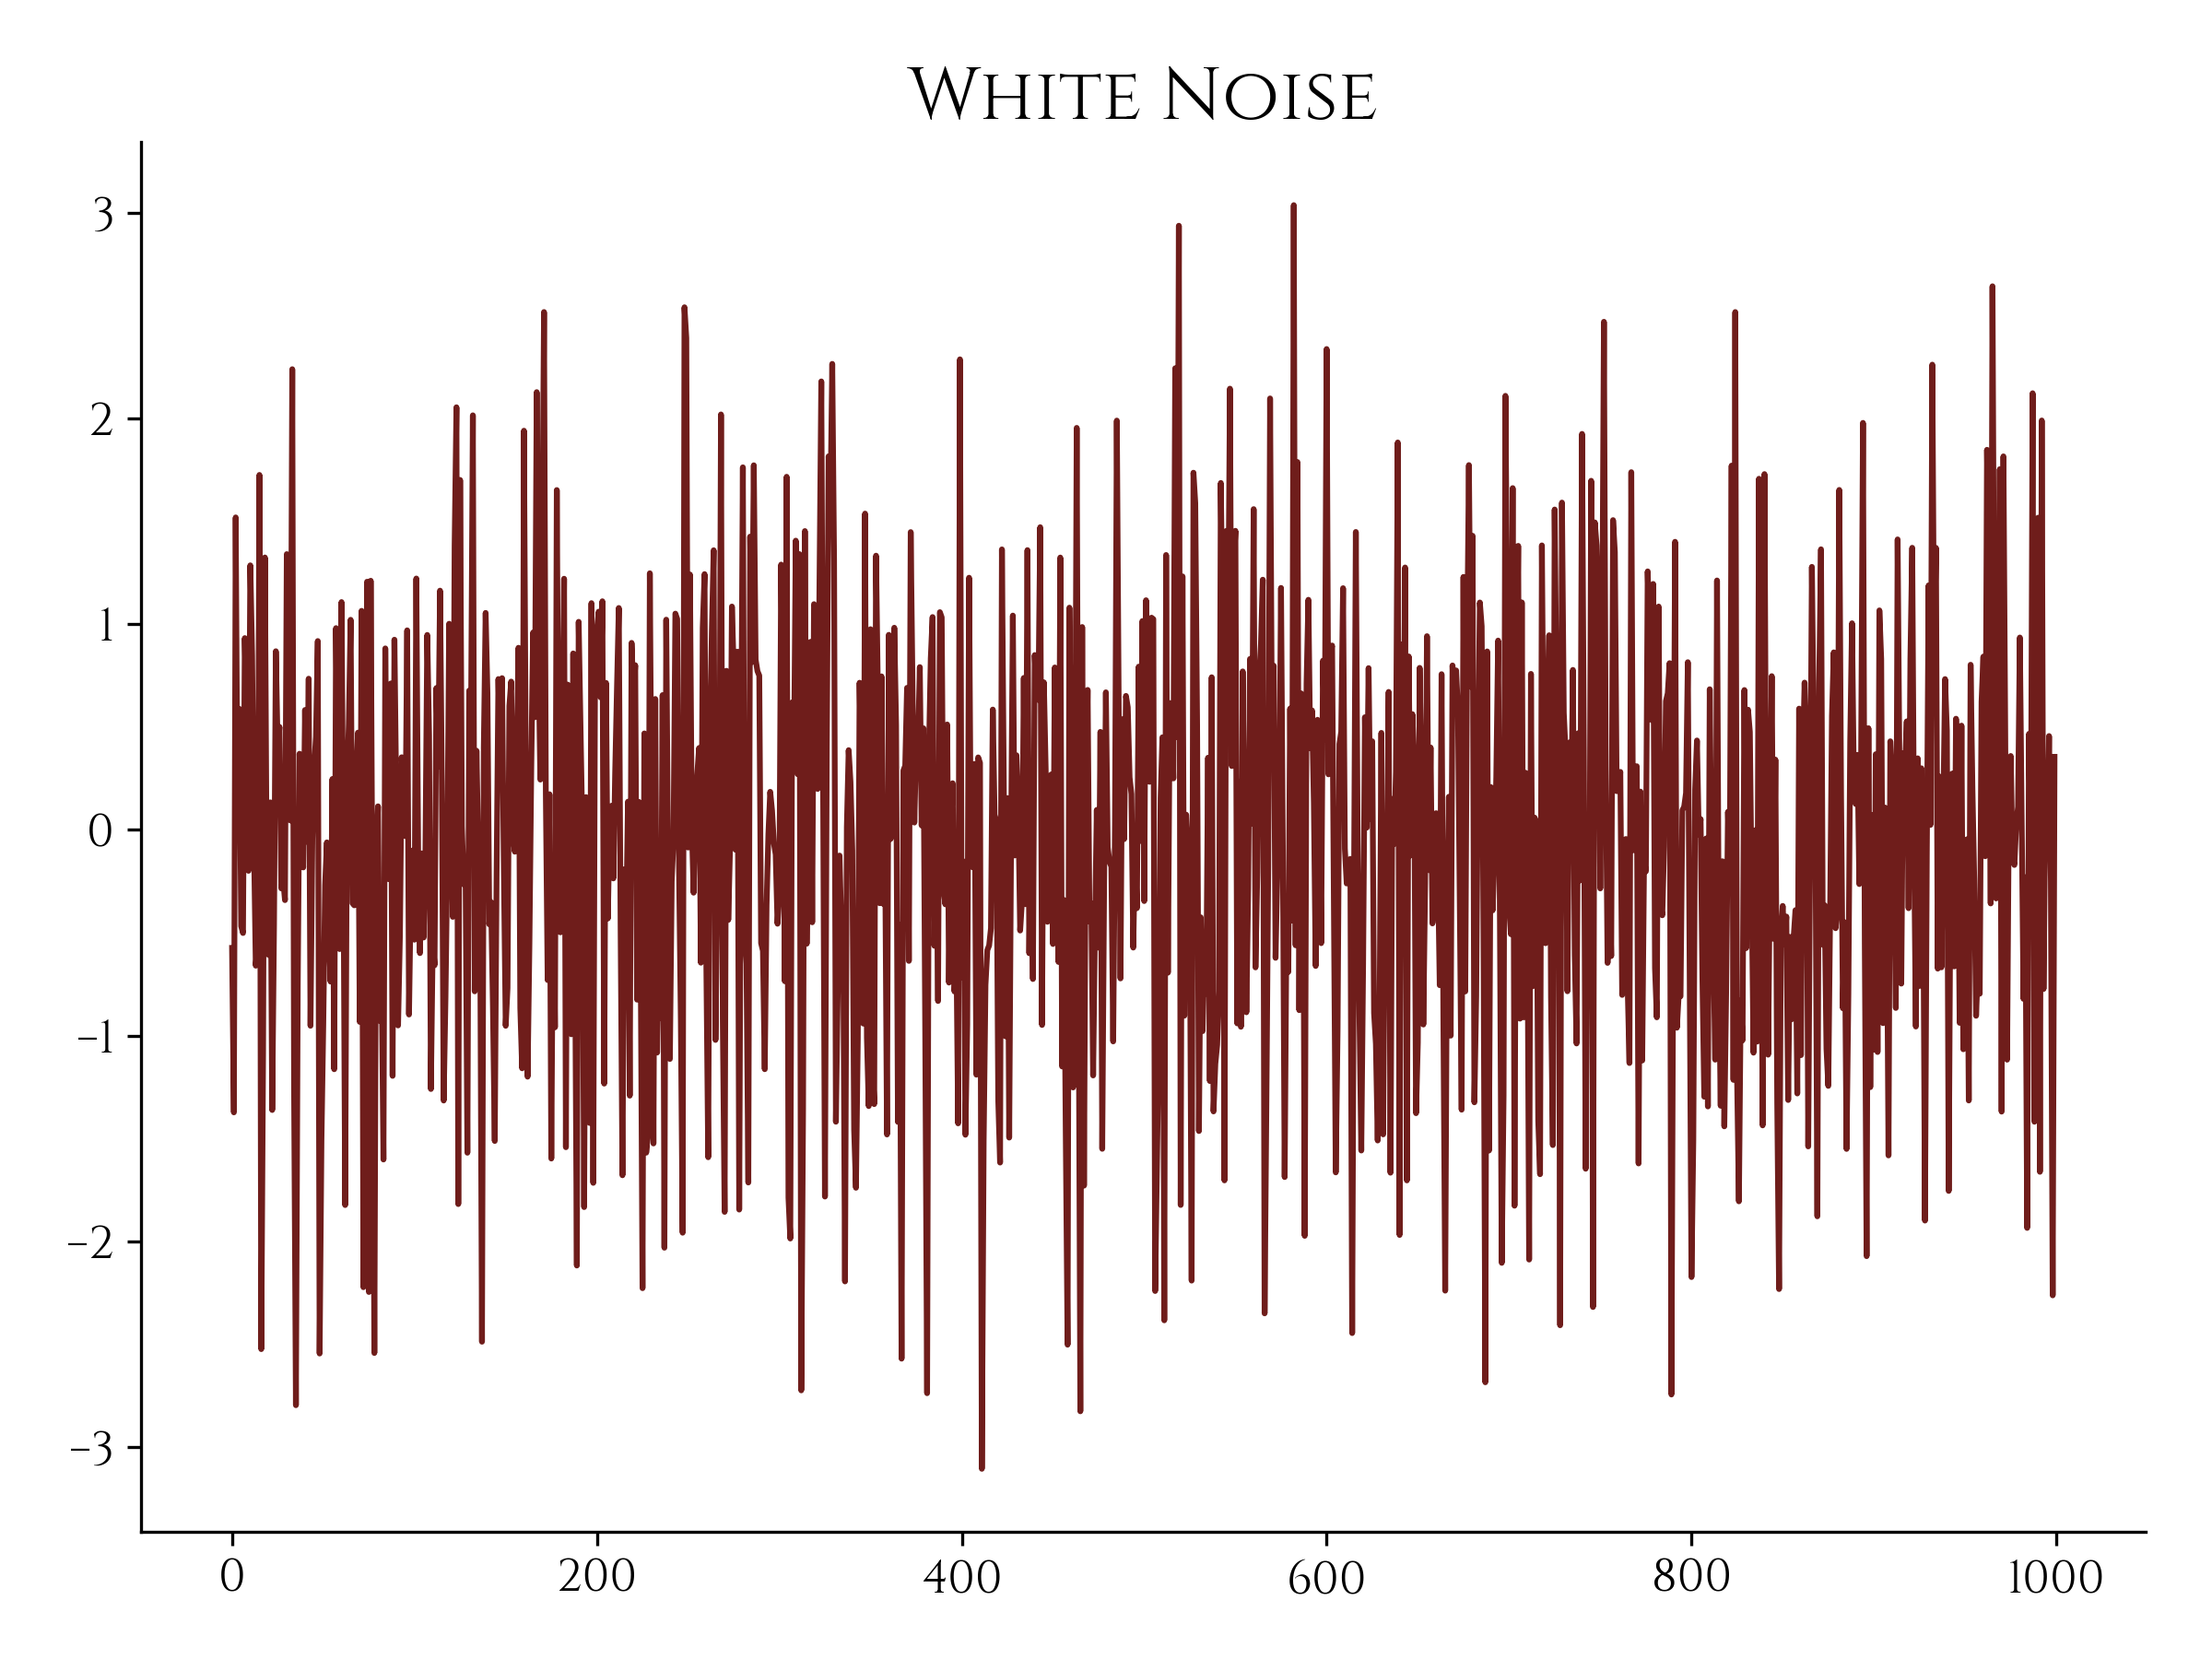
\includegraphics[width=0.3\textwidth, keepaspectratio]{time_series_example_random_small}}
    \hfill
    \subcaptionbox{листинг \ref{lst:time_series_example_wine} \label{fig:time_series_example_wine_small}}[0.3\textwidth]{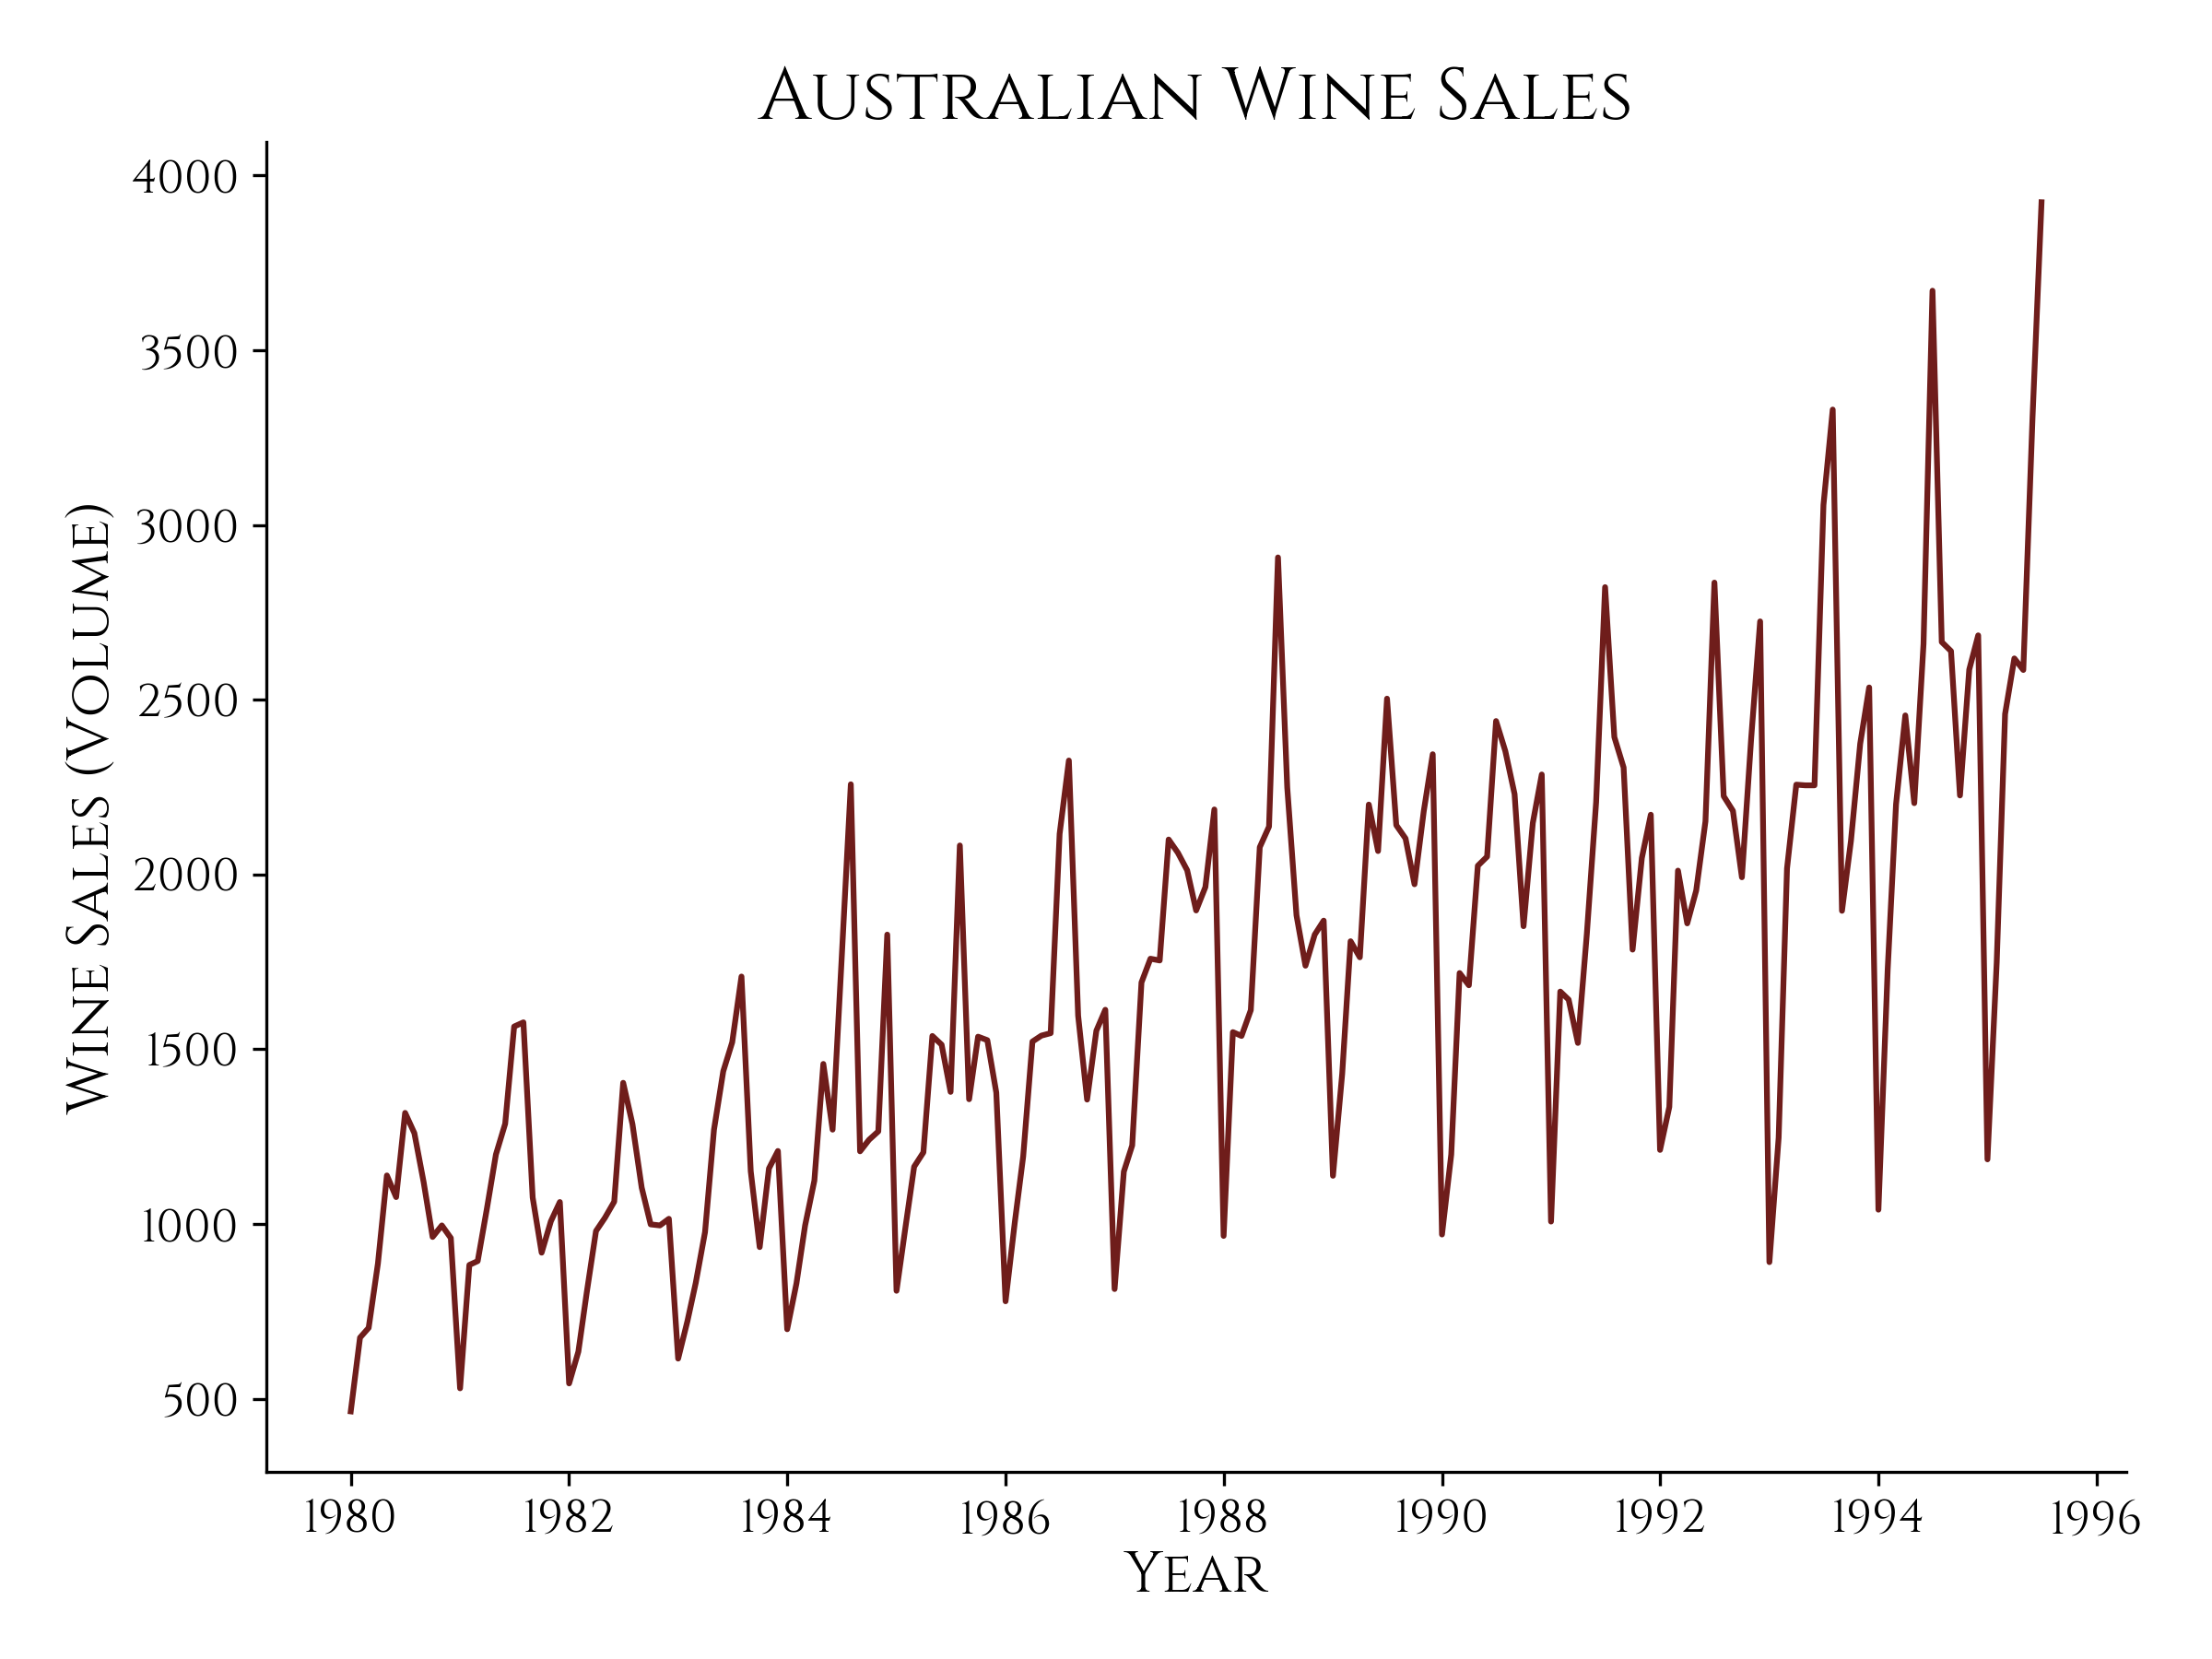
\includegraphics[width=0.3\textwidth, keepaspectratio]{time_series_example_wine_small}}
    
    % Second Row (add vertical spacing)
    \vspace{0.5cm}
    \subcaptionbox{листинг \ref{lst:time_series_example_gold_small} \label{fig:time_series_example_gold_small}}[0.3\textwidth]{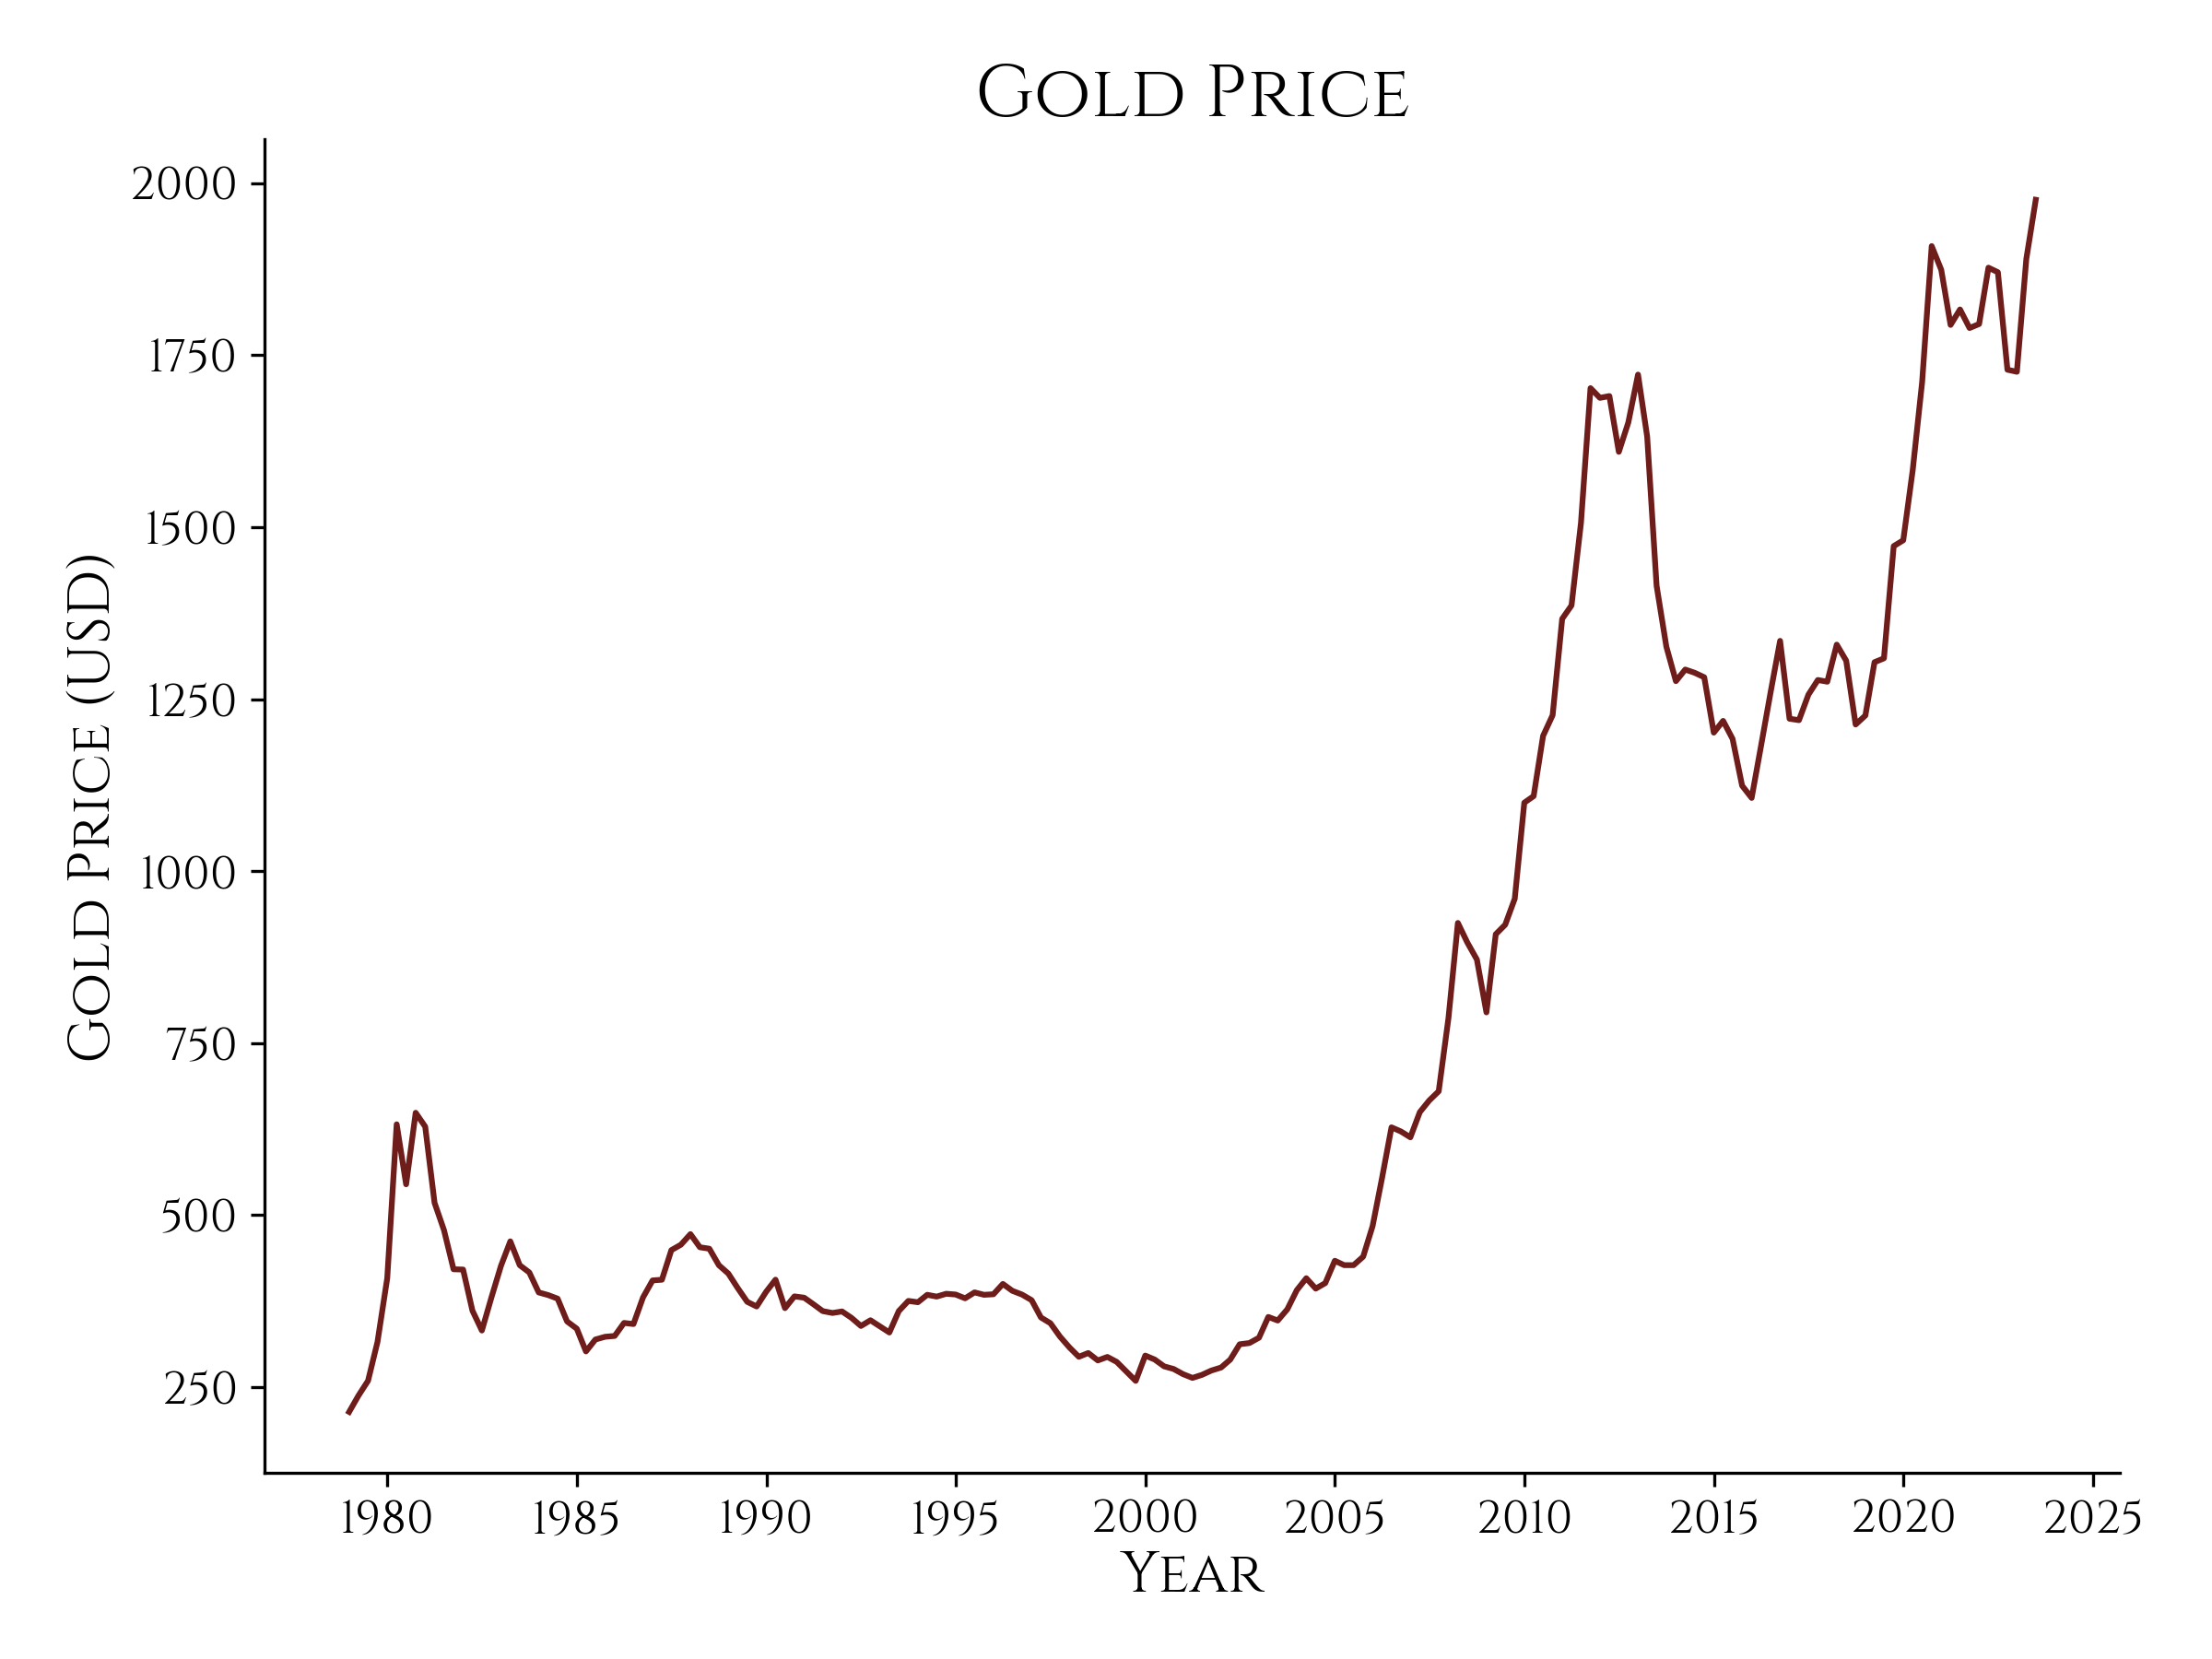
\includegraphics[width=0.3\textwidth, keepaspectratio]{time_series_example_gold_small}}
    \hfill
    \subcaptionbox{листинг \ref{lst:time_series_example_France} \label{fig:time_series_example_France_small}}[0.3\textwidth]{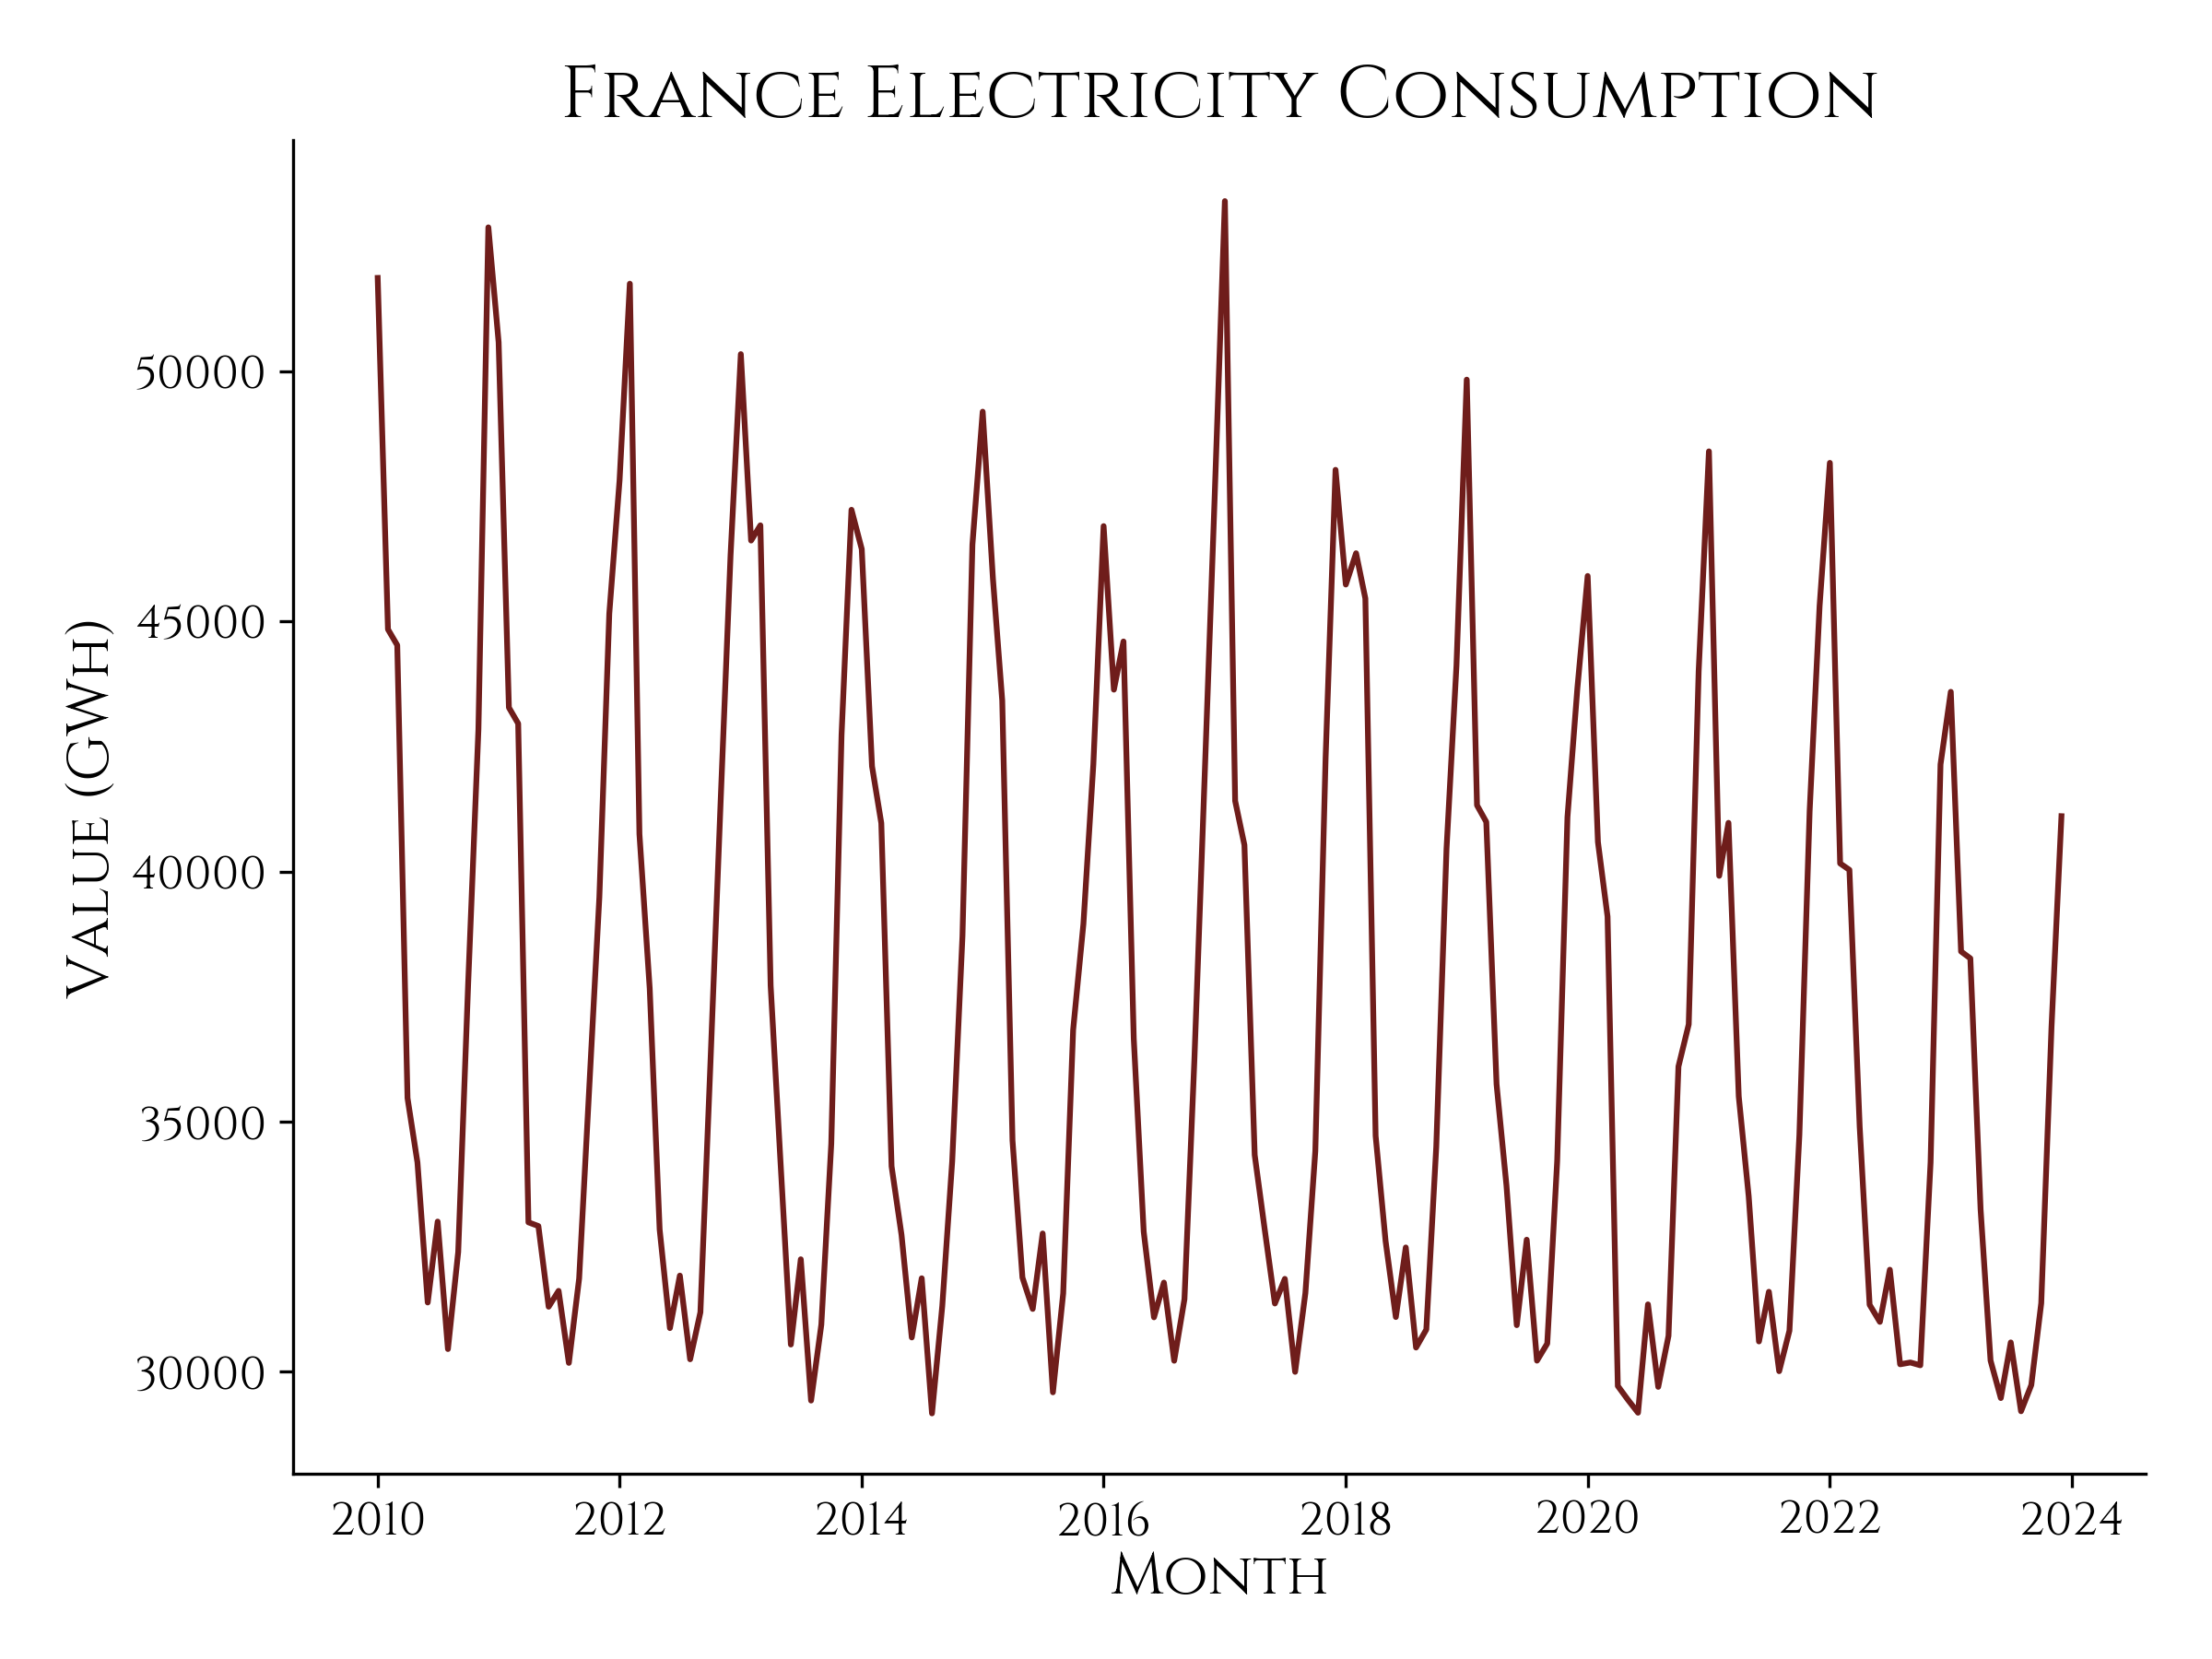
\includegraphics[width=0.3\textwidth, keepaspectratio]{time_series_example_France_small}}
    \hfill
    \subcaptionbox{листинг \ref{lst:time_series_example_Dow_Jones_small} \label{fig:time_series_example_Dow_Jones_small}}[0.3\textwidth]{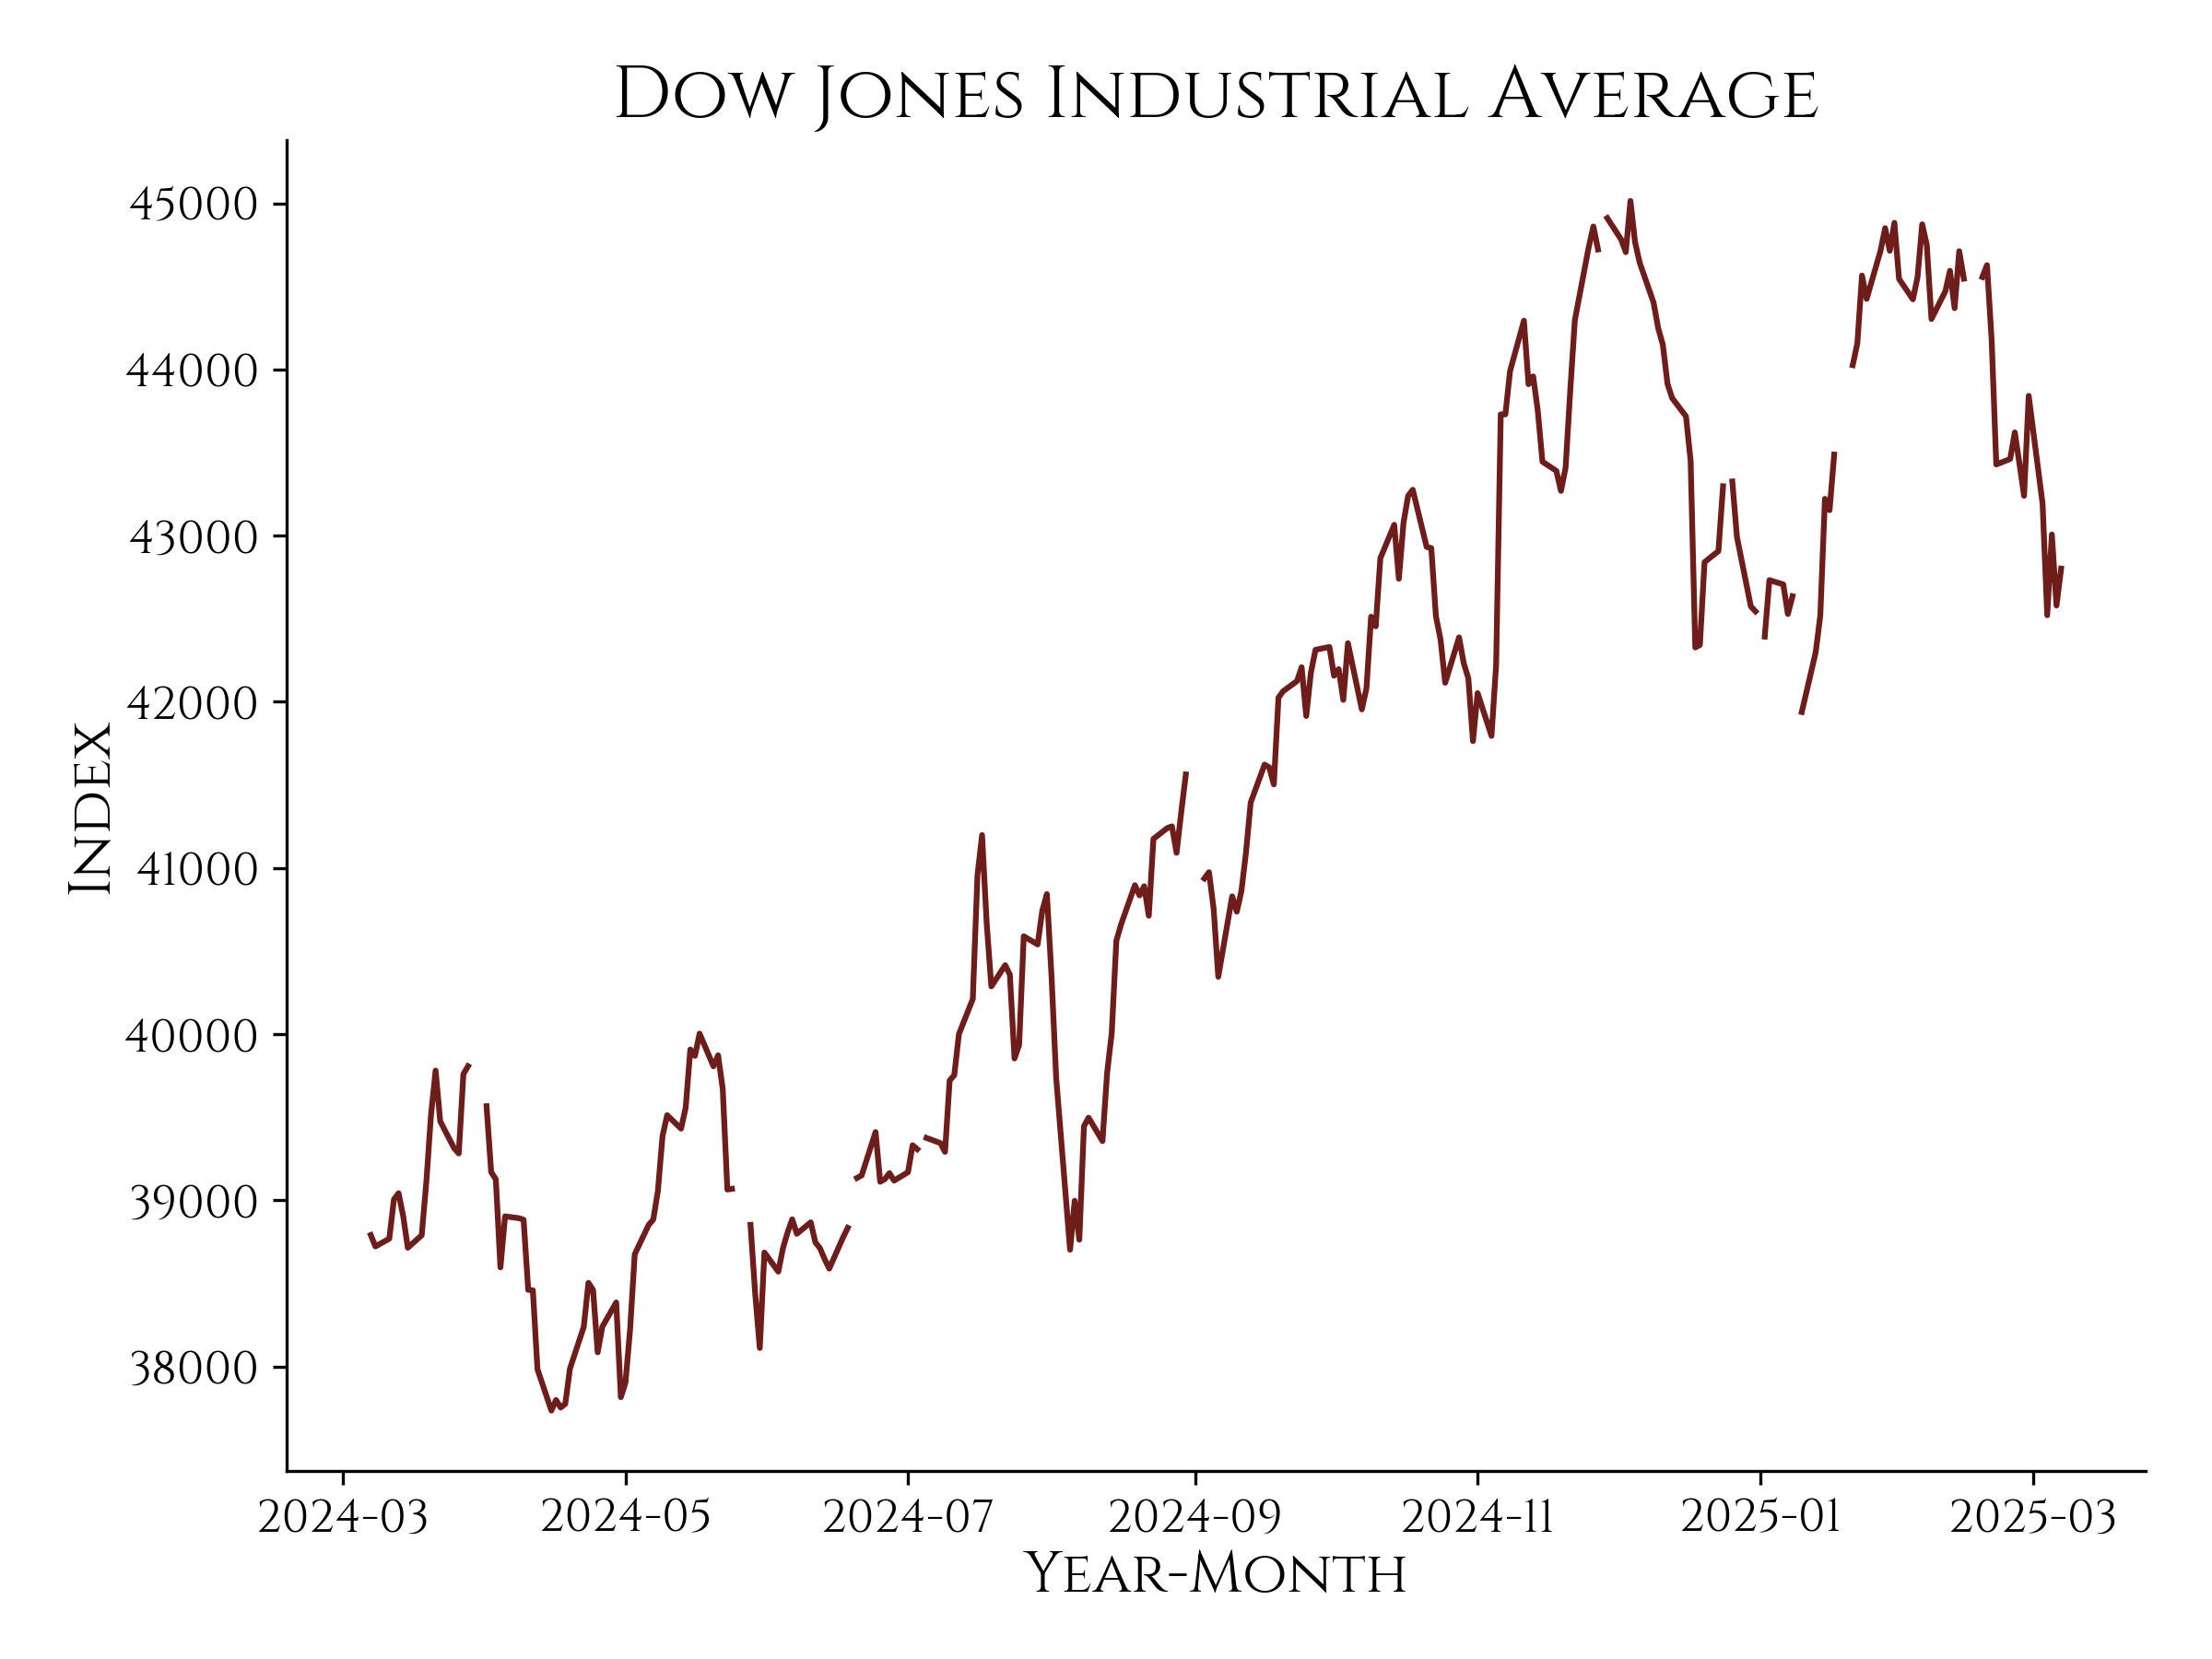
\includegraphics[width=0.3\textwidth, keepaspectratio]{time_series_example_Dow_Jones_small}}
    
    % Third Row (add vertical spacing)
    \vspace{0.5cm}
    \subcaptionbox{листинг \ref{lst:time_series_example_Dow_Jones_change_small} \label{fig:time_series_example_Dow_Jones_change_small}}[0.3\textwidth]{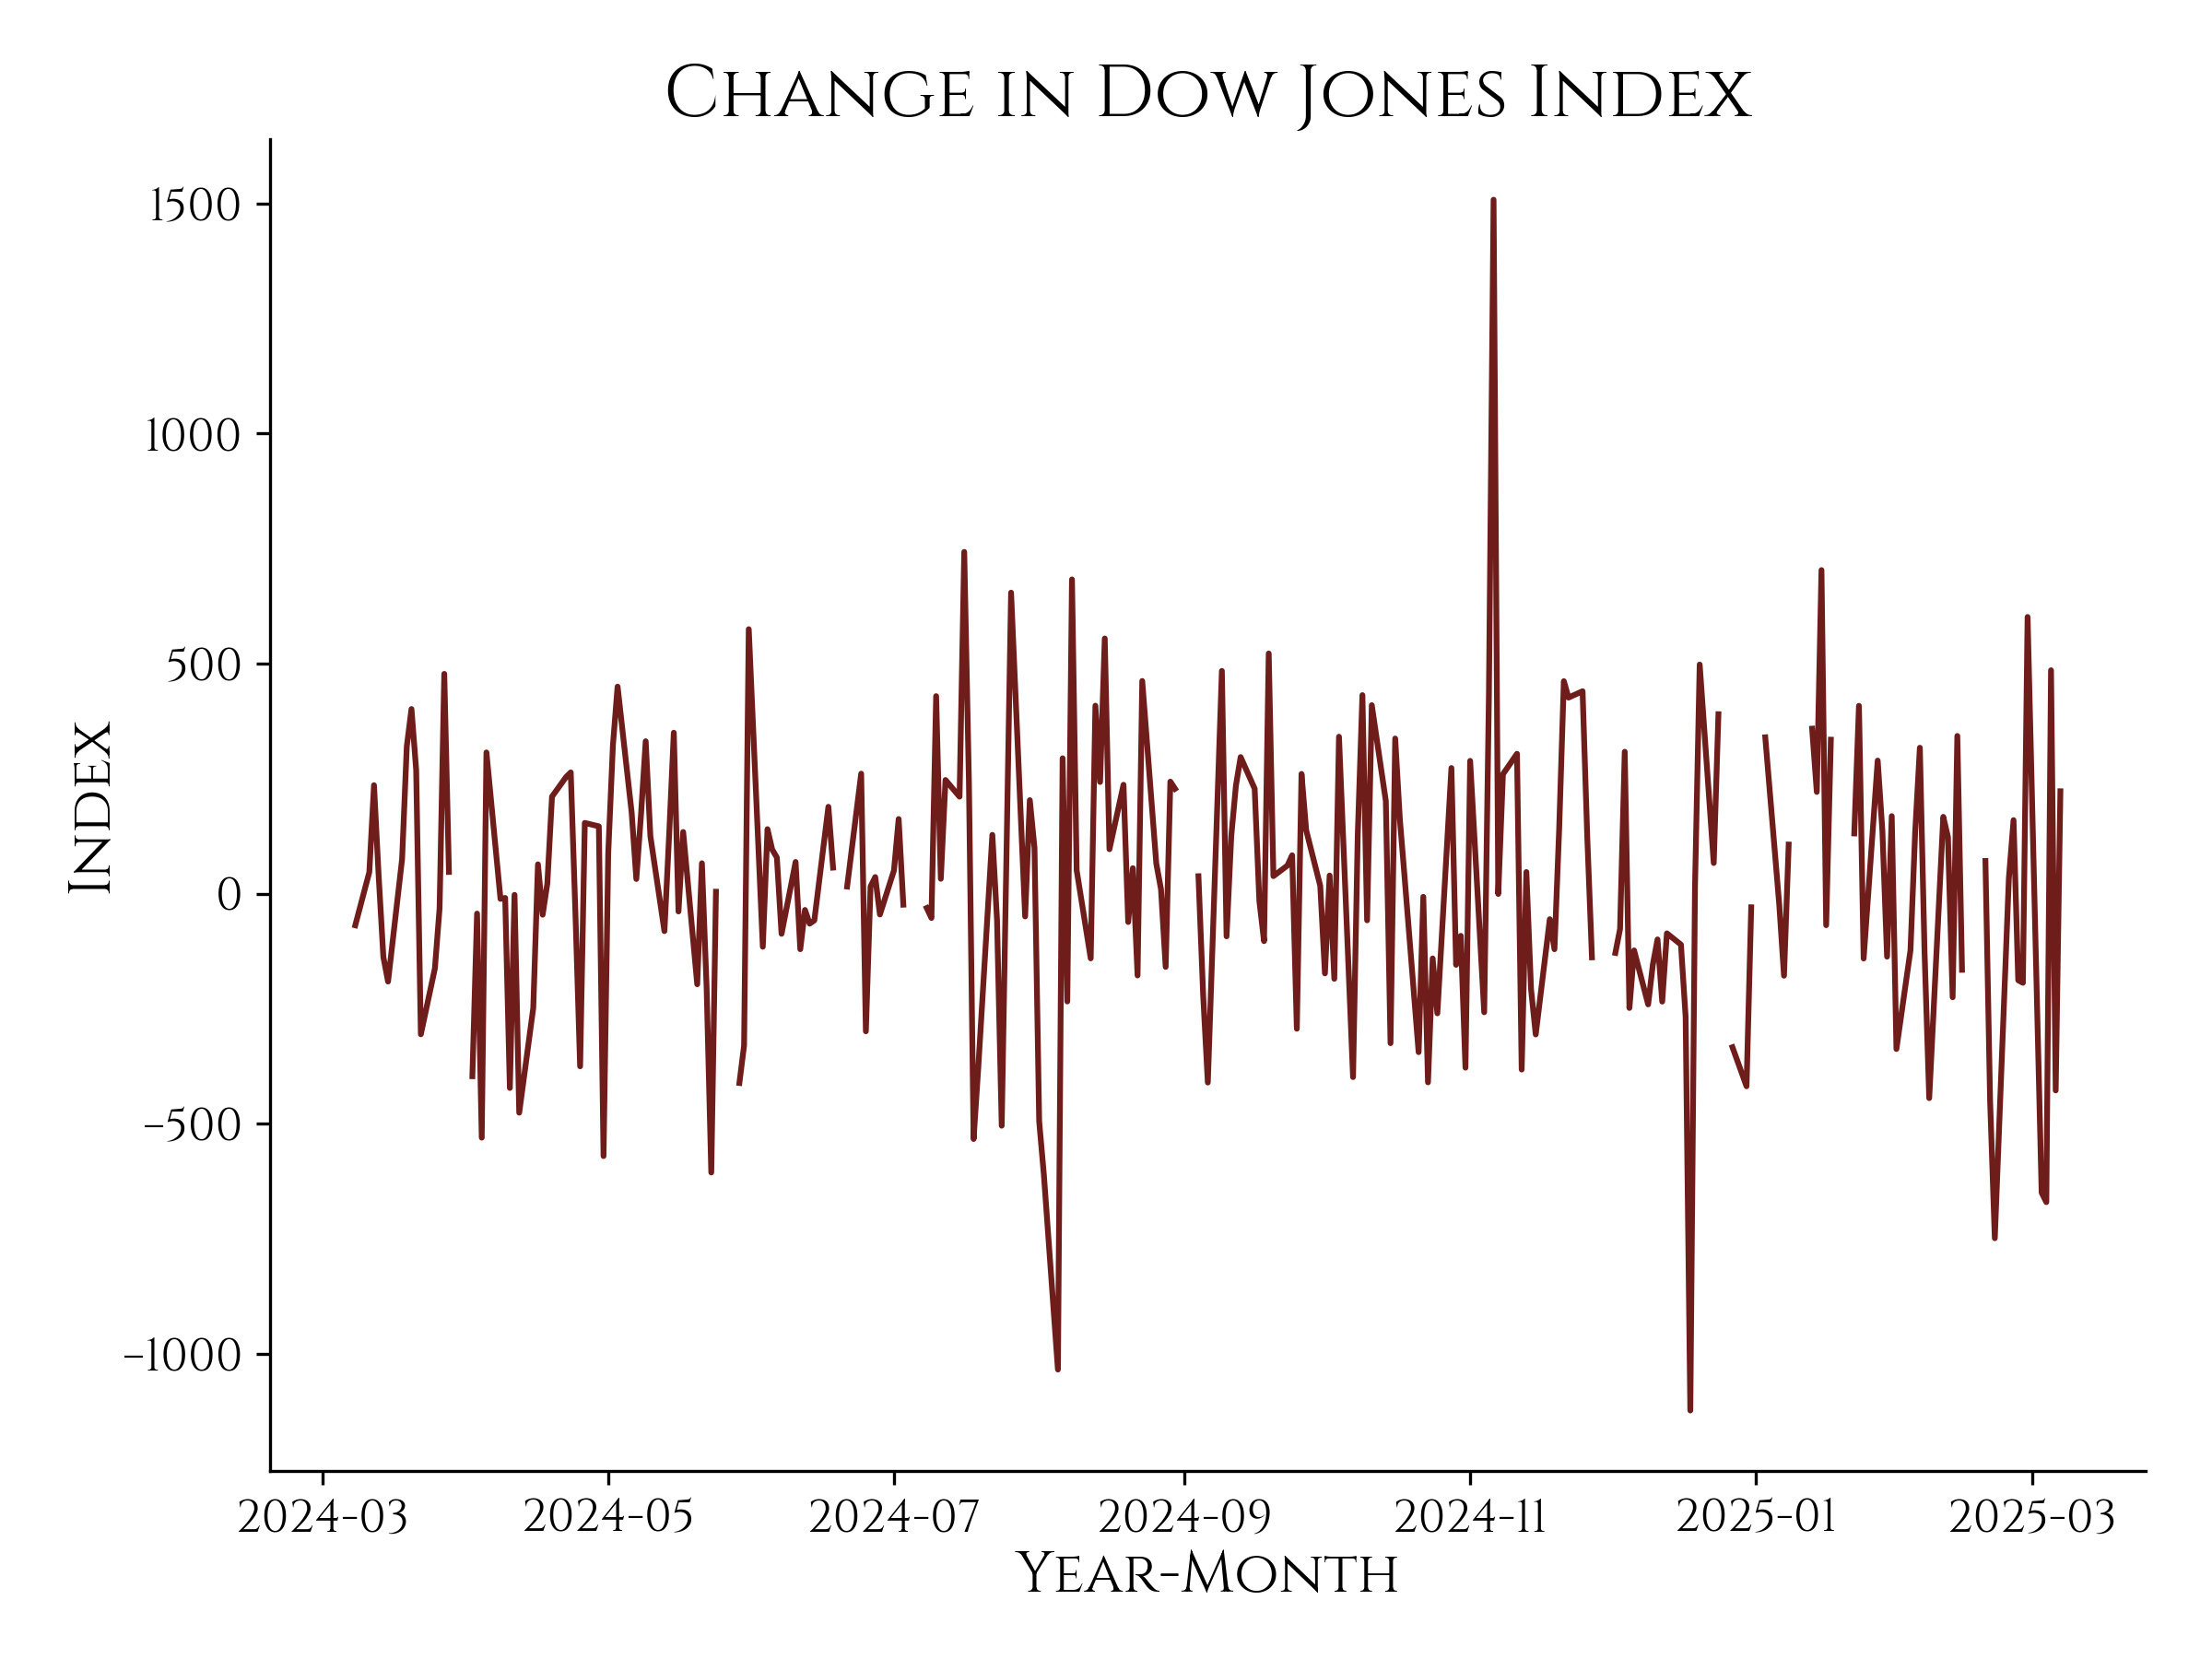
\includegraphics[width=0.3\textwidth, keepaspectratio]{time_series_example_Dow_Jones_change_small}}
    \hfill
    \subcaptionbox{листинг \ref{lst:time_series_example_sunspots_small} \label{fig:time_series_example_sunspots_small}}[0.3\textwidth]{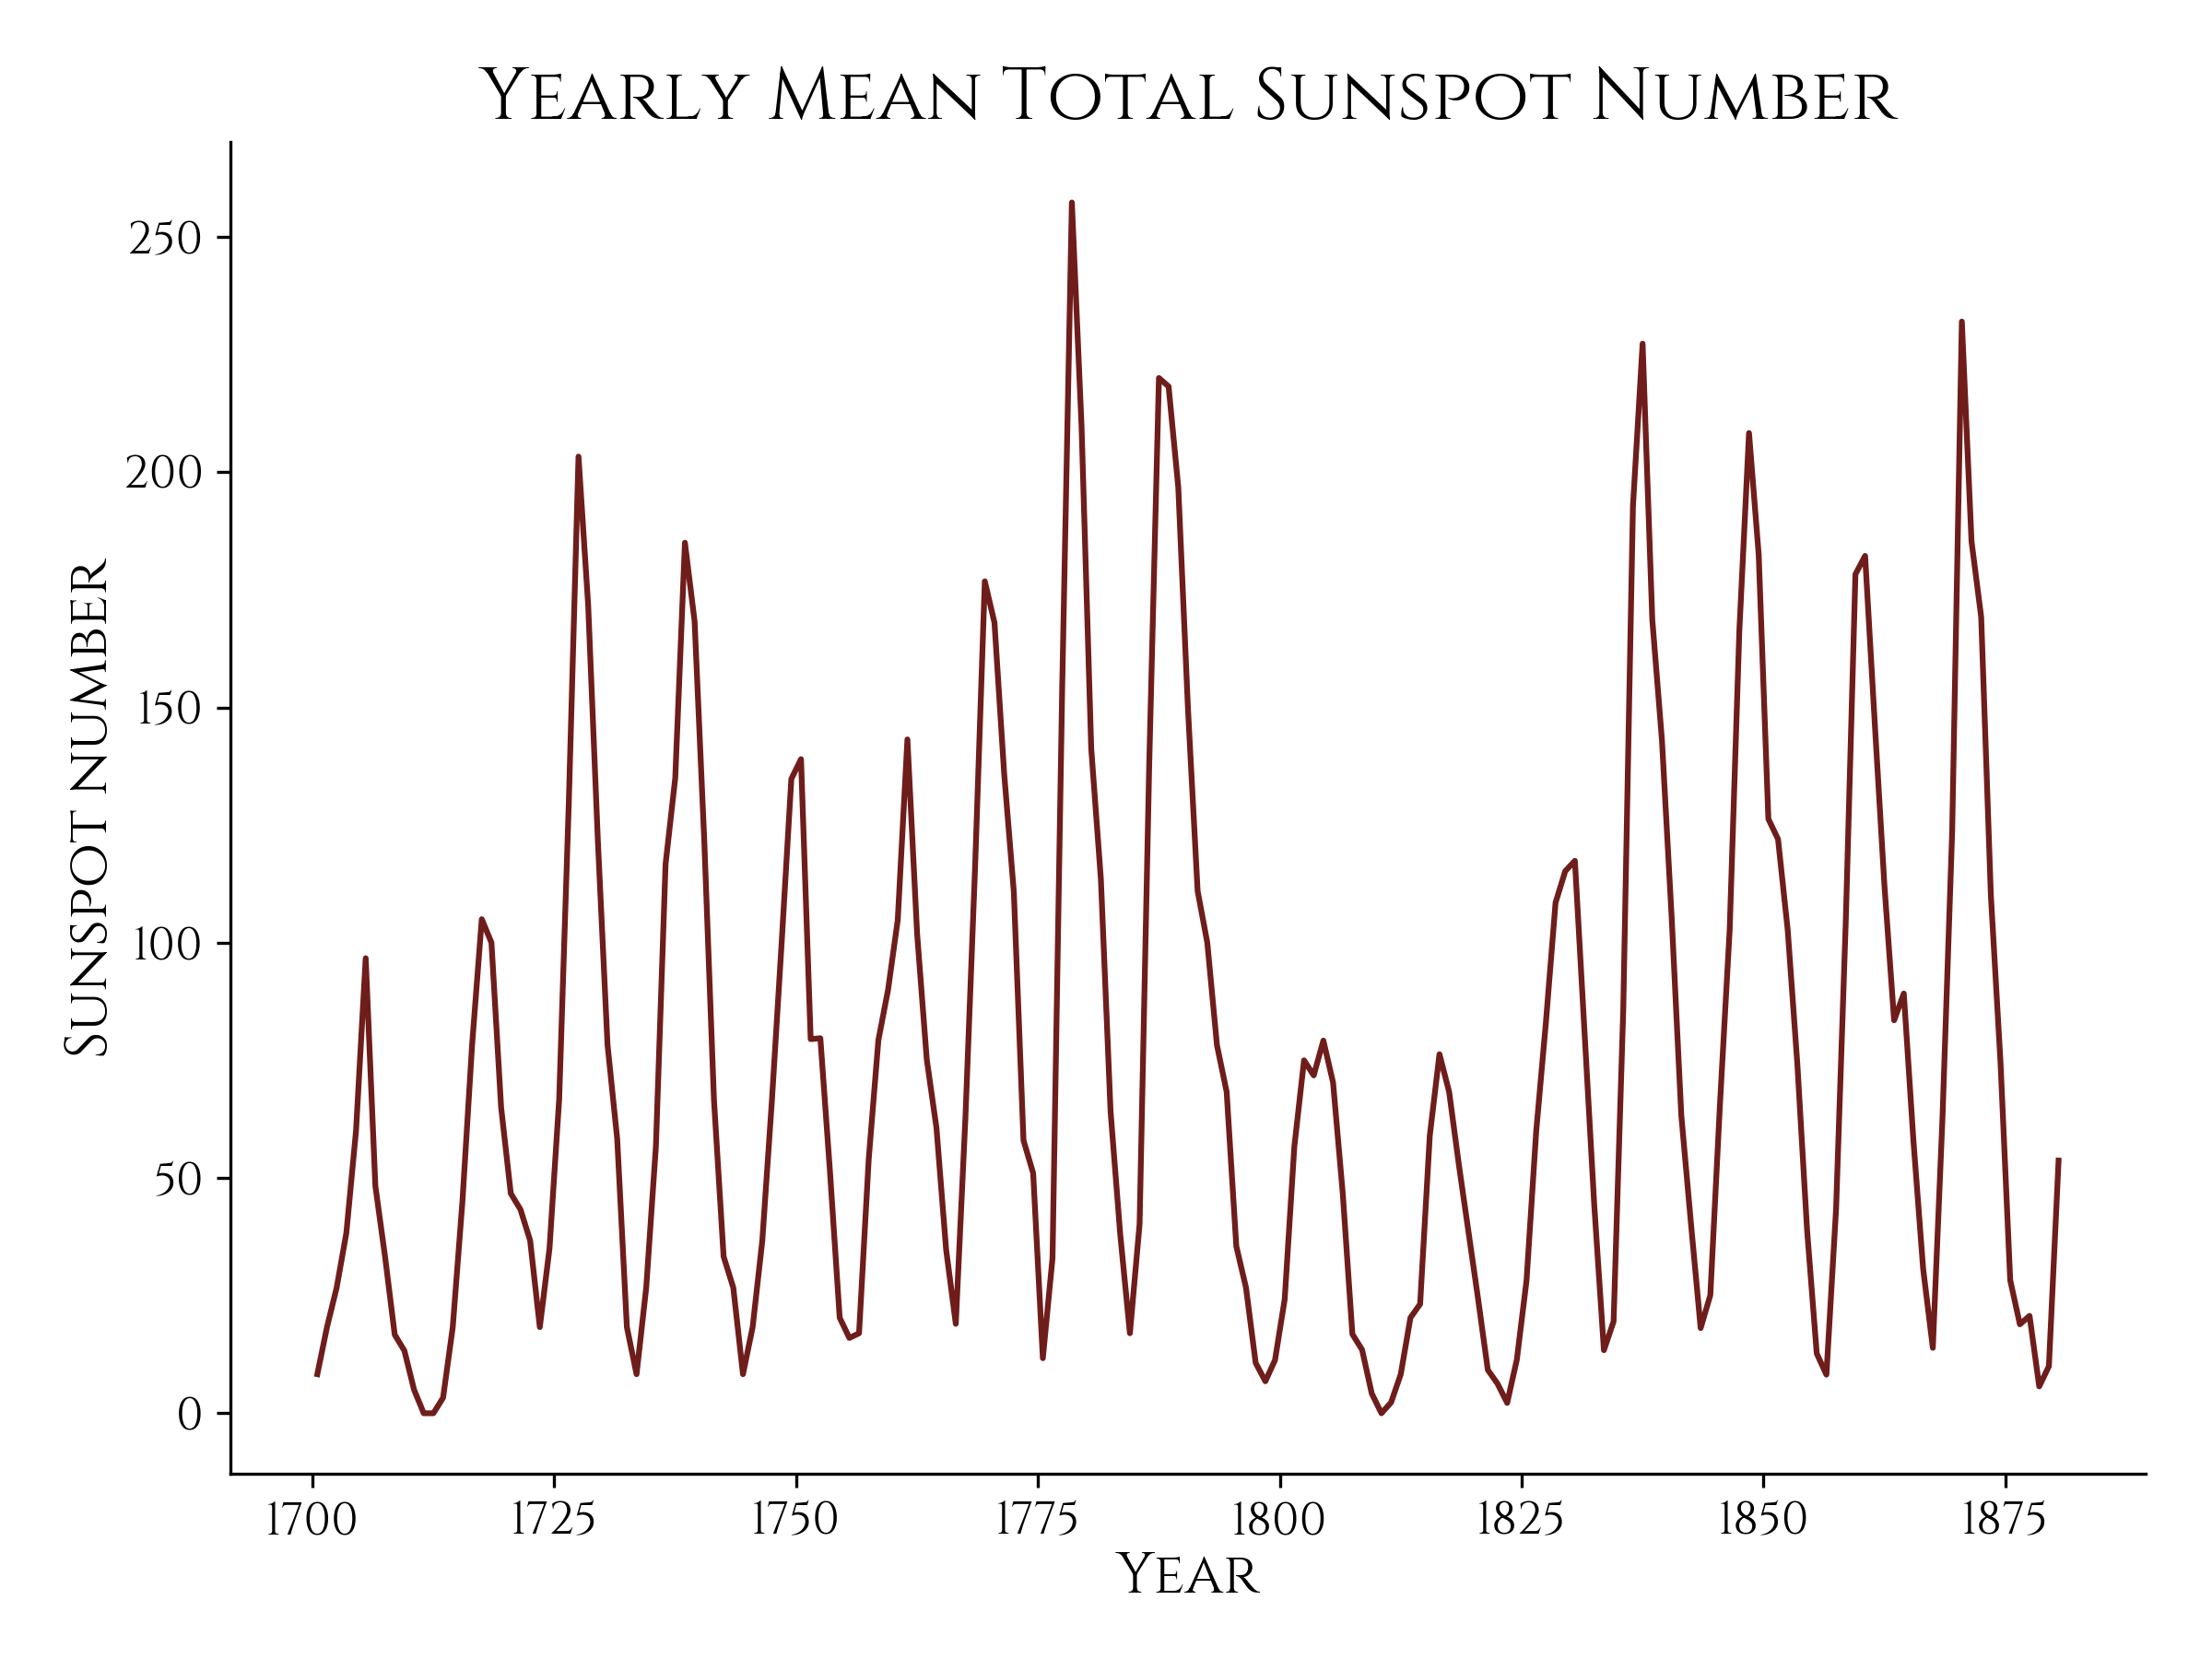
\includegraphics[width=0.3\textwidth, keepaspectratio]{time_series_example_sunspots_small}}
    \hfill
    \subcaptionbox{листинг \ref{lst:time_series_example_airline_small} \label{fig:time_series_example_airline_small}}[0.3\textwidth]{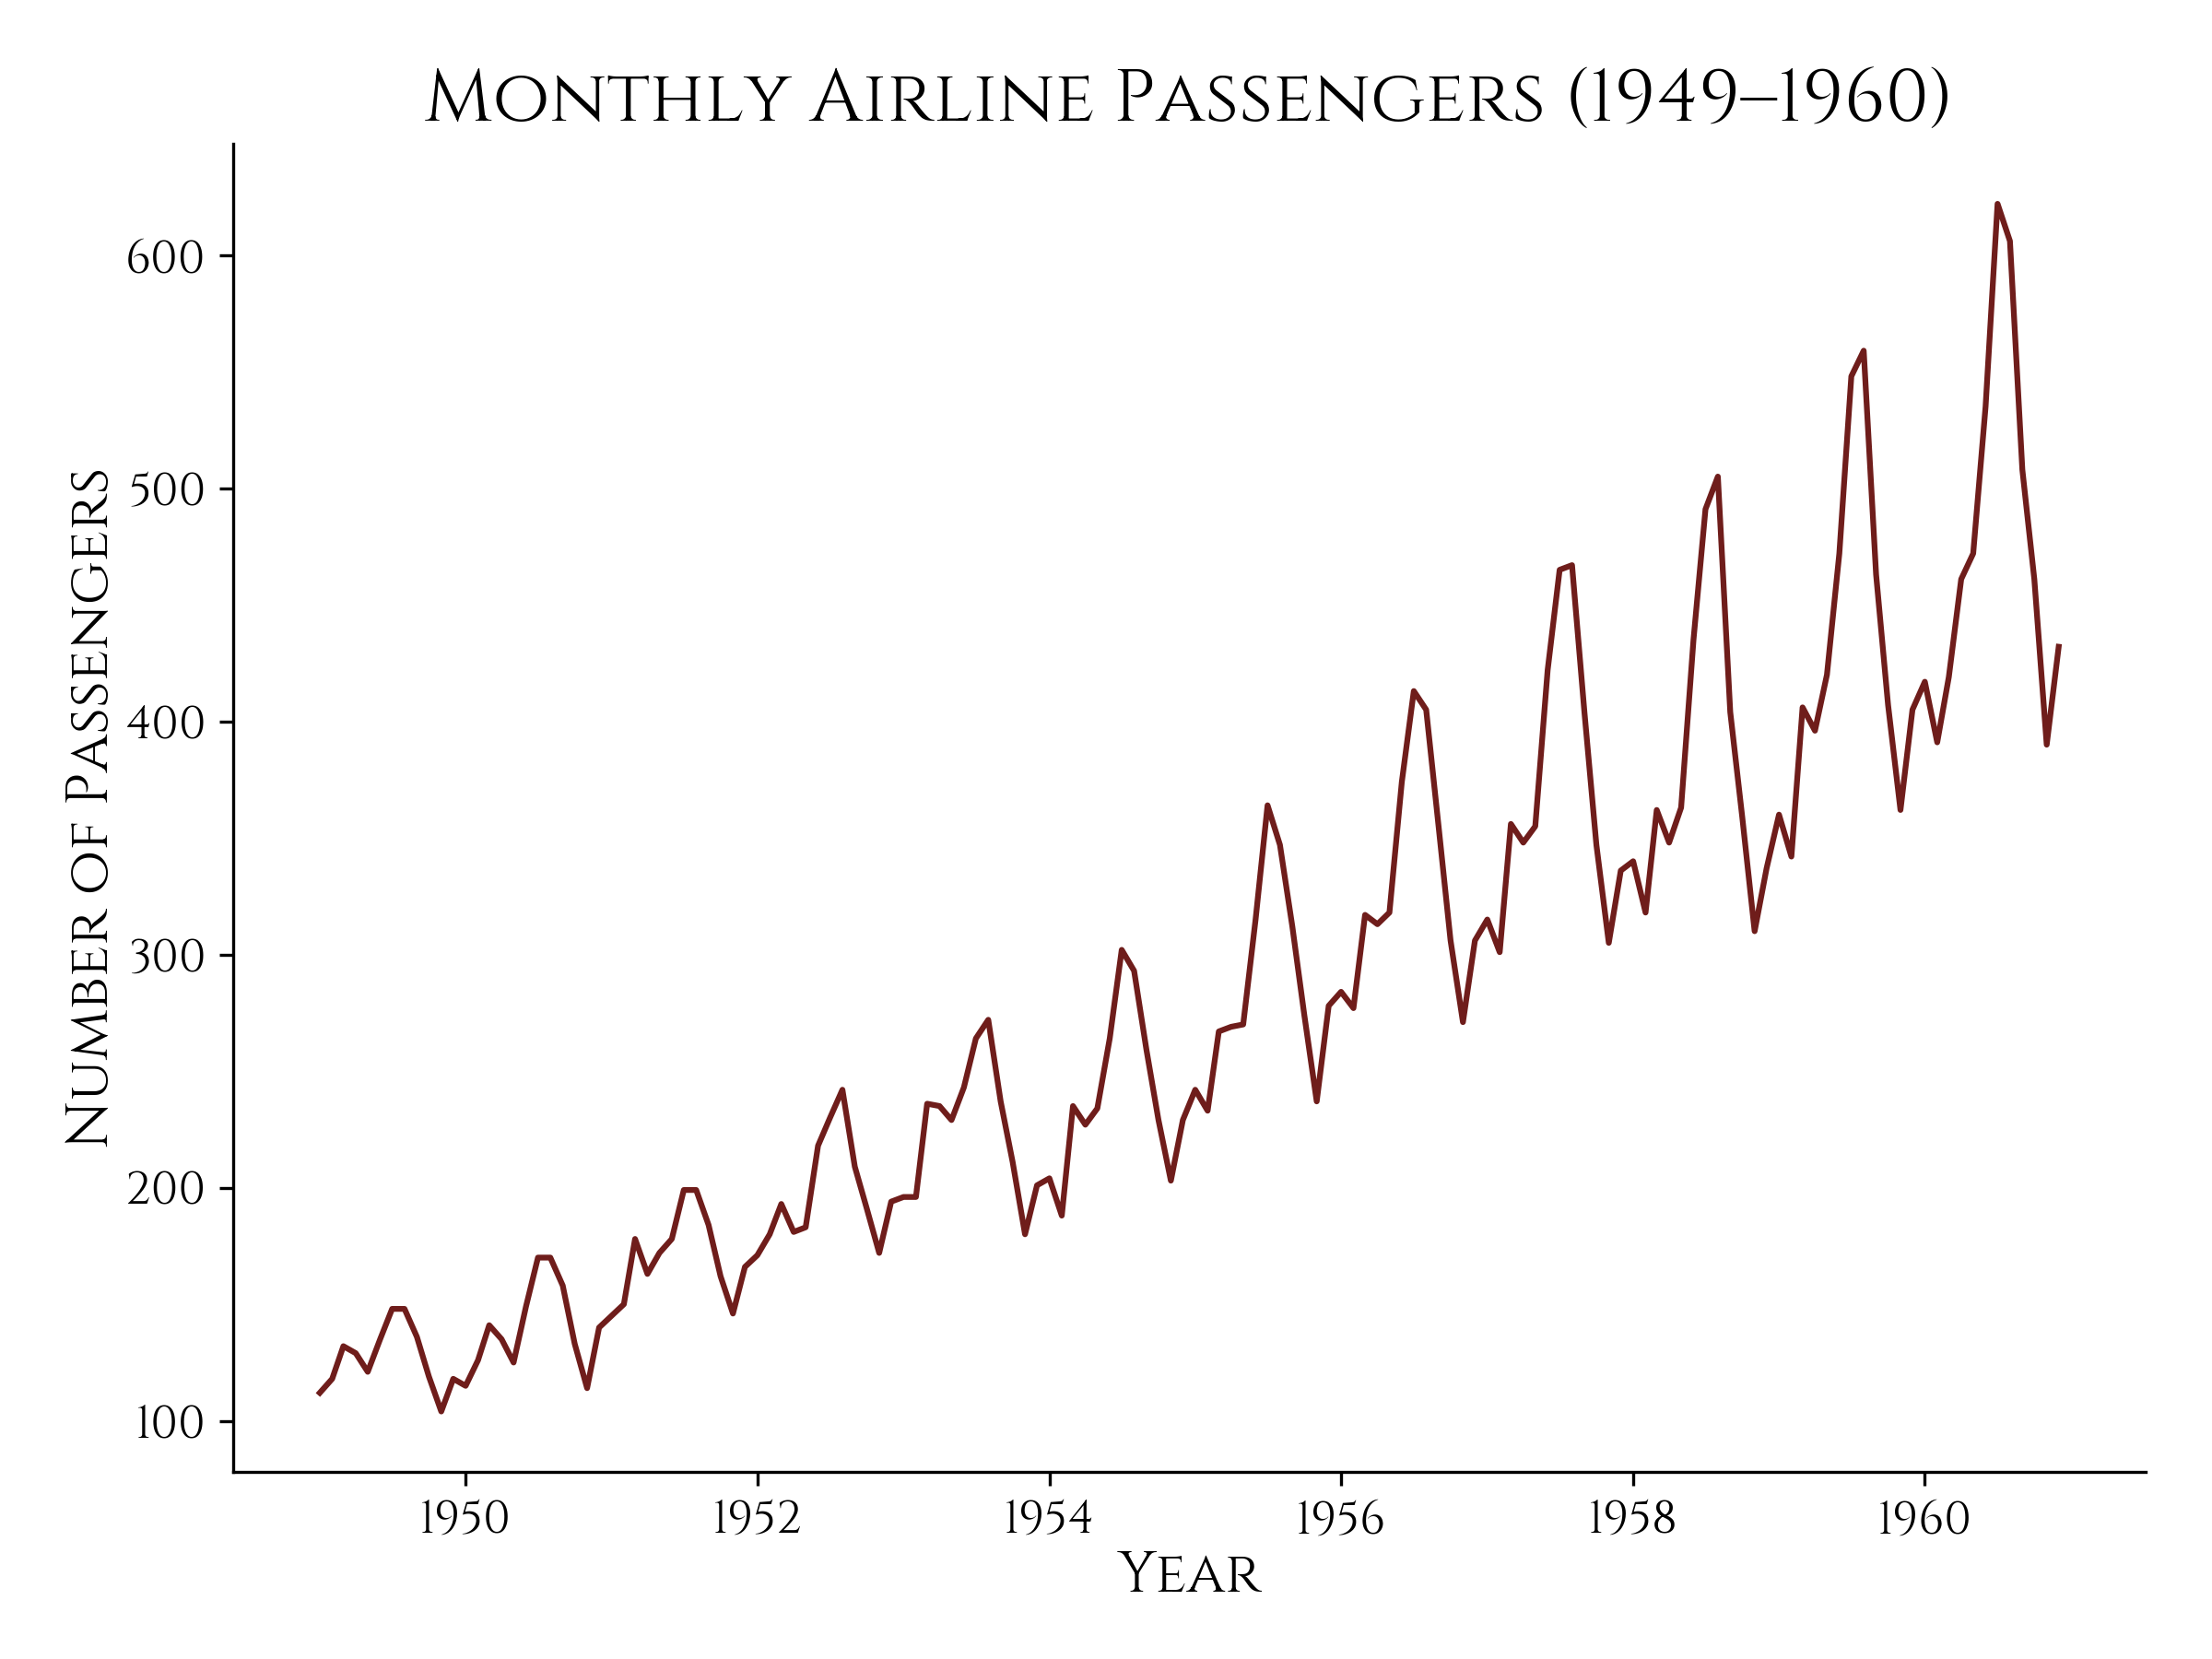
\includegraphics[width=0.3\textwidth, keepaspectratio]{time_series_example_airline_small}}

    \caption{Примеры временных рядов}
    \label{fig:time_series_examples}
\end{figure}

\newpage 
В качестве примера стационарных и нестационарных можно рассмотреть временные ряды, показанные на
рисунке 
\ref{fig:time_series_examples}. Ряды 
\ref{fig:time_series_example_wine_small}, 
\ref{fig:time_series_example_gold_small}, 
\ref{fig:time_series_example_France_small}, 
\ref{fig:time_series_example_Dow_Jones_small}, 
\ref{fig:time_series_example_airline_small} 
нестационарны из-за сильно выраженного тренда. В рядах 
\ref{fig:time_series_example_avocado_small}, 
\ref{fig:time_series_example_wine_small}, 
\ref{fig:time_series_example_France_small}, 
\ref{fig:time_series_example_airline_small} 
сильно выражена сезонность, поэтому они также нестационарны. В ряду 
\ref{fig:time_series_example_airline_small}, 
помимо всего прочего, меняется и дисперсия (т.е. присутствует, ещё одно свойство, не постоянное по времени). 
Остаются три ряда, 
\ref{fig:time_series_example_random_small}, 
\ref{fig:time_series_example_Dow_Jones_change_small} и 
\ref{fig:time_series_example_sunspots_small}.

Первый - это просто белый шум, который по определению стационарен, второй - ежедневное изменение индекса Доу-Джонса, 
этот ряд также считается стационарным, а третий - среднегодовое общее количество солнечных пятен. 

Третий временной ряд является классическим примером нестационарного ряда с периодическим поведением. 
Истинная стационарность требует постоянного среднего и дисперсии, что отсутствует у среднего 
ежегодного количества солнечных пятен в связи изменяющимися амплитудами циклов. Однако некоторые 
исследователи считают цикличность за, своего рода, \guillemotleft квази-стационарность\guillemotright \cite{Forecasting_Brockwell}.\\

Формально:

\noindent\rule{\linewidth}{0.1mm}

\begin{definition}
    Пусть $\left\{ X_t \right\}$ - временной ряд с 
    $\mathbb{E}\left[ X_t^2 \right] < \infty$. Тогда \textbf{функцией среднего} 
    от $\left\{ X_t \right\}$ называется выражение вида:
    \vspace{-10pt}
    \begin{equation*}
        \mu_X(t) = \mathbb{E} \left[ X_t \right].
    \end{equation*}
    \vspace{-20pt}
    В свою очередь \textbf{ковариационной функцией} от $\left\{ X_t \right\}$ называется:
    \begin{equation*}
        \gamma_X (r, s) = \text{Cov}(X_r, X_s) = \mathbb{E}\left[ (X_r - \mu_x (r)) 
        (X_s - \mu_X (s)) \right]
    \end{equation*}
    \vspace{-20pt}
    для всех целых чисел $r$ и $s$.\\
\end{definition}

\noindent\rule{\linewidth}{0.1mm}

\begin{definition}
    $\left\{ X_t \right\}$ называется (\textbf{слабо}) 
    \textbf{стационарным} если
    \begin{itemize}
        \item $\mu_X(t)$ не зависит от времени $t$,
    \end{itemize}
    \vspace{-10pt}
    и 
    \vspace{-10pt}
    \begin{itemize}
        \item $\gamma_X(t+h, t)$ не зависит от времени $t$ для каждого $h$.
    \end{itemize}
    \noindent\rule{\linewidth}{0.1mm}
\end{definition}

\noindent\textbf{Примечание} Строгая стационарность временного ряда $\left\{ 
X_t, t = 0, \pm 1, \dots \right\}$ определяется условием об одинаковом 
совместном распределении
$ \left( X_1, \dots, X_n \right) $ и $ \left( X_{1+h}, \dots, X_{n+h} \right) $ 
для всех $h$ и $n > 0$ $\in \mathbb{Z}$.

\subsubsection{Тесты на единичный корень}

В качестве формальной проверки временных рядов на стационарность было 
разработано множество различных тестов. Среди них есть 
параметрические тесты (тесты на единичный корень (unit root tests) как 
раз входят в их число), полу-параметрические и непараметриечские. 
Рассмотрим некоторые из семейства тестов на единичные корни (так как 
на практике чаще всего встречаются именно они):

\begin{itemize}
    \item \textbf{Тесты Дики-Фуллера} - семейство статистических тестов для проверки 
    нулевой гипотезы о наличии единичного корня (unit root) в модели авторегрессии 
    (см. главу [\textcolor{red}{TODO}]) рассматриваемого временного ряда, и что процесс, таким образом, 
    является нестационарным. Альтернативная гипотеза меняется в зависимости от 
    вариации используемого теста. На практике часто используется расширенный 
    тест Дики-Фуллера (ADF).

    \item \textbf{Критерий KPSS} (Kwiatkowski–Phillips–Schmidt–Shin) - тест, 
    в котором наличие единичного корня является альтернативной гипотезой. 
    В качестве нулевой гипотезы рассматривают стационарность временного ряда.
    
    \item  \textbf{Тест DF-GLS} (Dickey-Fuller Generalized Least Squares) - 
    модификация ADF, где тренд удаляется с помощью 
    обобщенного метода наименьших квадратов. Как и в ADF, 
    нулевая гипотеза - наличие единичного корня.
\end{itemize}

\subsubsection{Дифференцирование}

Так как для работы во многих моделях от временного ряда требуется стационарность - 
были разработаны методы сведения нестационарных временных рядов к стационарным. 
Вспомним, что ранее расмотренный индекс Доу-Джонса (рис. \ref{fig:time_series_example_Dow_Jones_small}) 
является нестационарным временным рядом, когда, в свою очередь, 
изменение в том же индексе Доу-Джонса (рис. \ref{fig:time_series_example_Dow_Jones_change_small}) 
уже считается стационарным. Это, как раз таки, демонстрирует 
один из методов сведения нестационарных временных рядов к стационарным - 
\textbf{дифференцирование}. \\

Дифференцированным рядом первого порядка называется ряд, состоящий из 
изменений между последовтельными 
наблюдениями в оригинальном временном ряду, и может быть записан в виде:
\begin{equation*}
    y'_t = y_t - y_{t-1}
\end{equation*} 

Но помимо дифференцирования первого порядка, есть и другие:
\begin{itemize}
    \item \textbf{Дифференцирование второго порядка}
    \begin{align*}
        y''_t &= y'_t - y'_{t-1}  \\
        &= (y_t - y_{t-1}) - (y_{t-1} - y_{t-2})  \\
        &= y_t - 2 y_{t-1} + y_{t-2}
    \end{align*}
    Очевидно, что идею дифференцирования можно обощить и на более 
    высокие порядки.
    \item \textbf{Сезонное дифференцирование}
    \begin{equation*}
        y_t = y_t - y_{t-m},
    \end{equation*}
    где $m$ - количество сезонов. (Подобное дифференцирование также называют 
    \guillemotleft разницами лага $m$\guillemotright {} (lag-$m$ differences)).
\end{itemize} 

\subsubsection{Преобразования}

Преобразования (transformation) чаще всего используются для стабилизации 
дисперсии временного ряда. Очень часто на практике используют семейство 
преобразований Бокса-Кокса:

\begin{equation*}
    y_i^{\lambda} = \begin{cases}
        \cfrac{y_i^{\lambda} - 1}{\lambda} \quad \lambda \neq 0 \\
    \ln(y_i) \quad \lambda = 0,
    \end{cases}
\end{equation*}
где $\lambda$ - параметр. \\

Помимо стабилизации дисперсии, преобразование Бокса-Кокса также помогает 
достичь нормализации и уменьшения перекоса (что позволяет сделать 
распределение более симметричным).\\

Рассмотрим преобразование Бокса-Кокса на примере ежемесячного 
количества пассажиров авиалиний с 1949 по 1960 года (рис. \ref{fig:time_series_example_airline_small2}):

\begin{center}
    \begin{minipage}{0.45\textwidth}
        \centering
        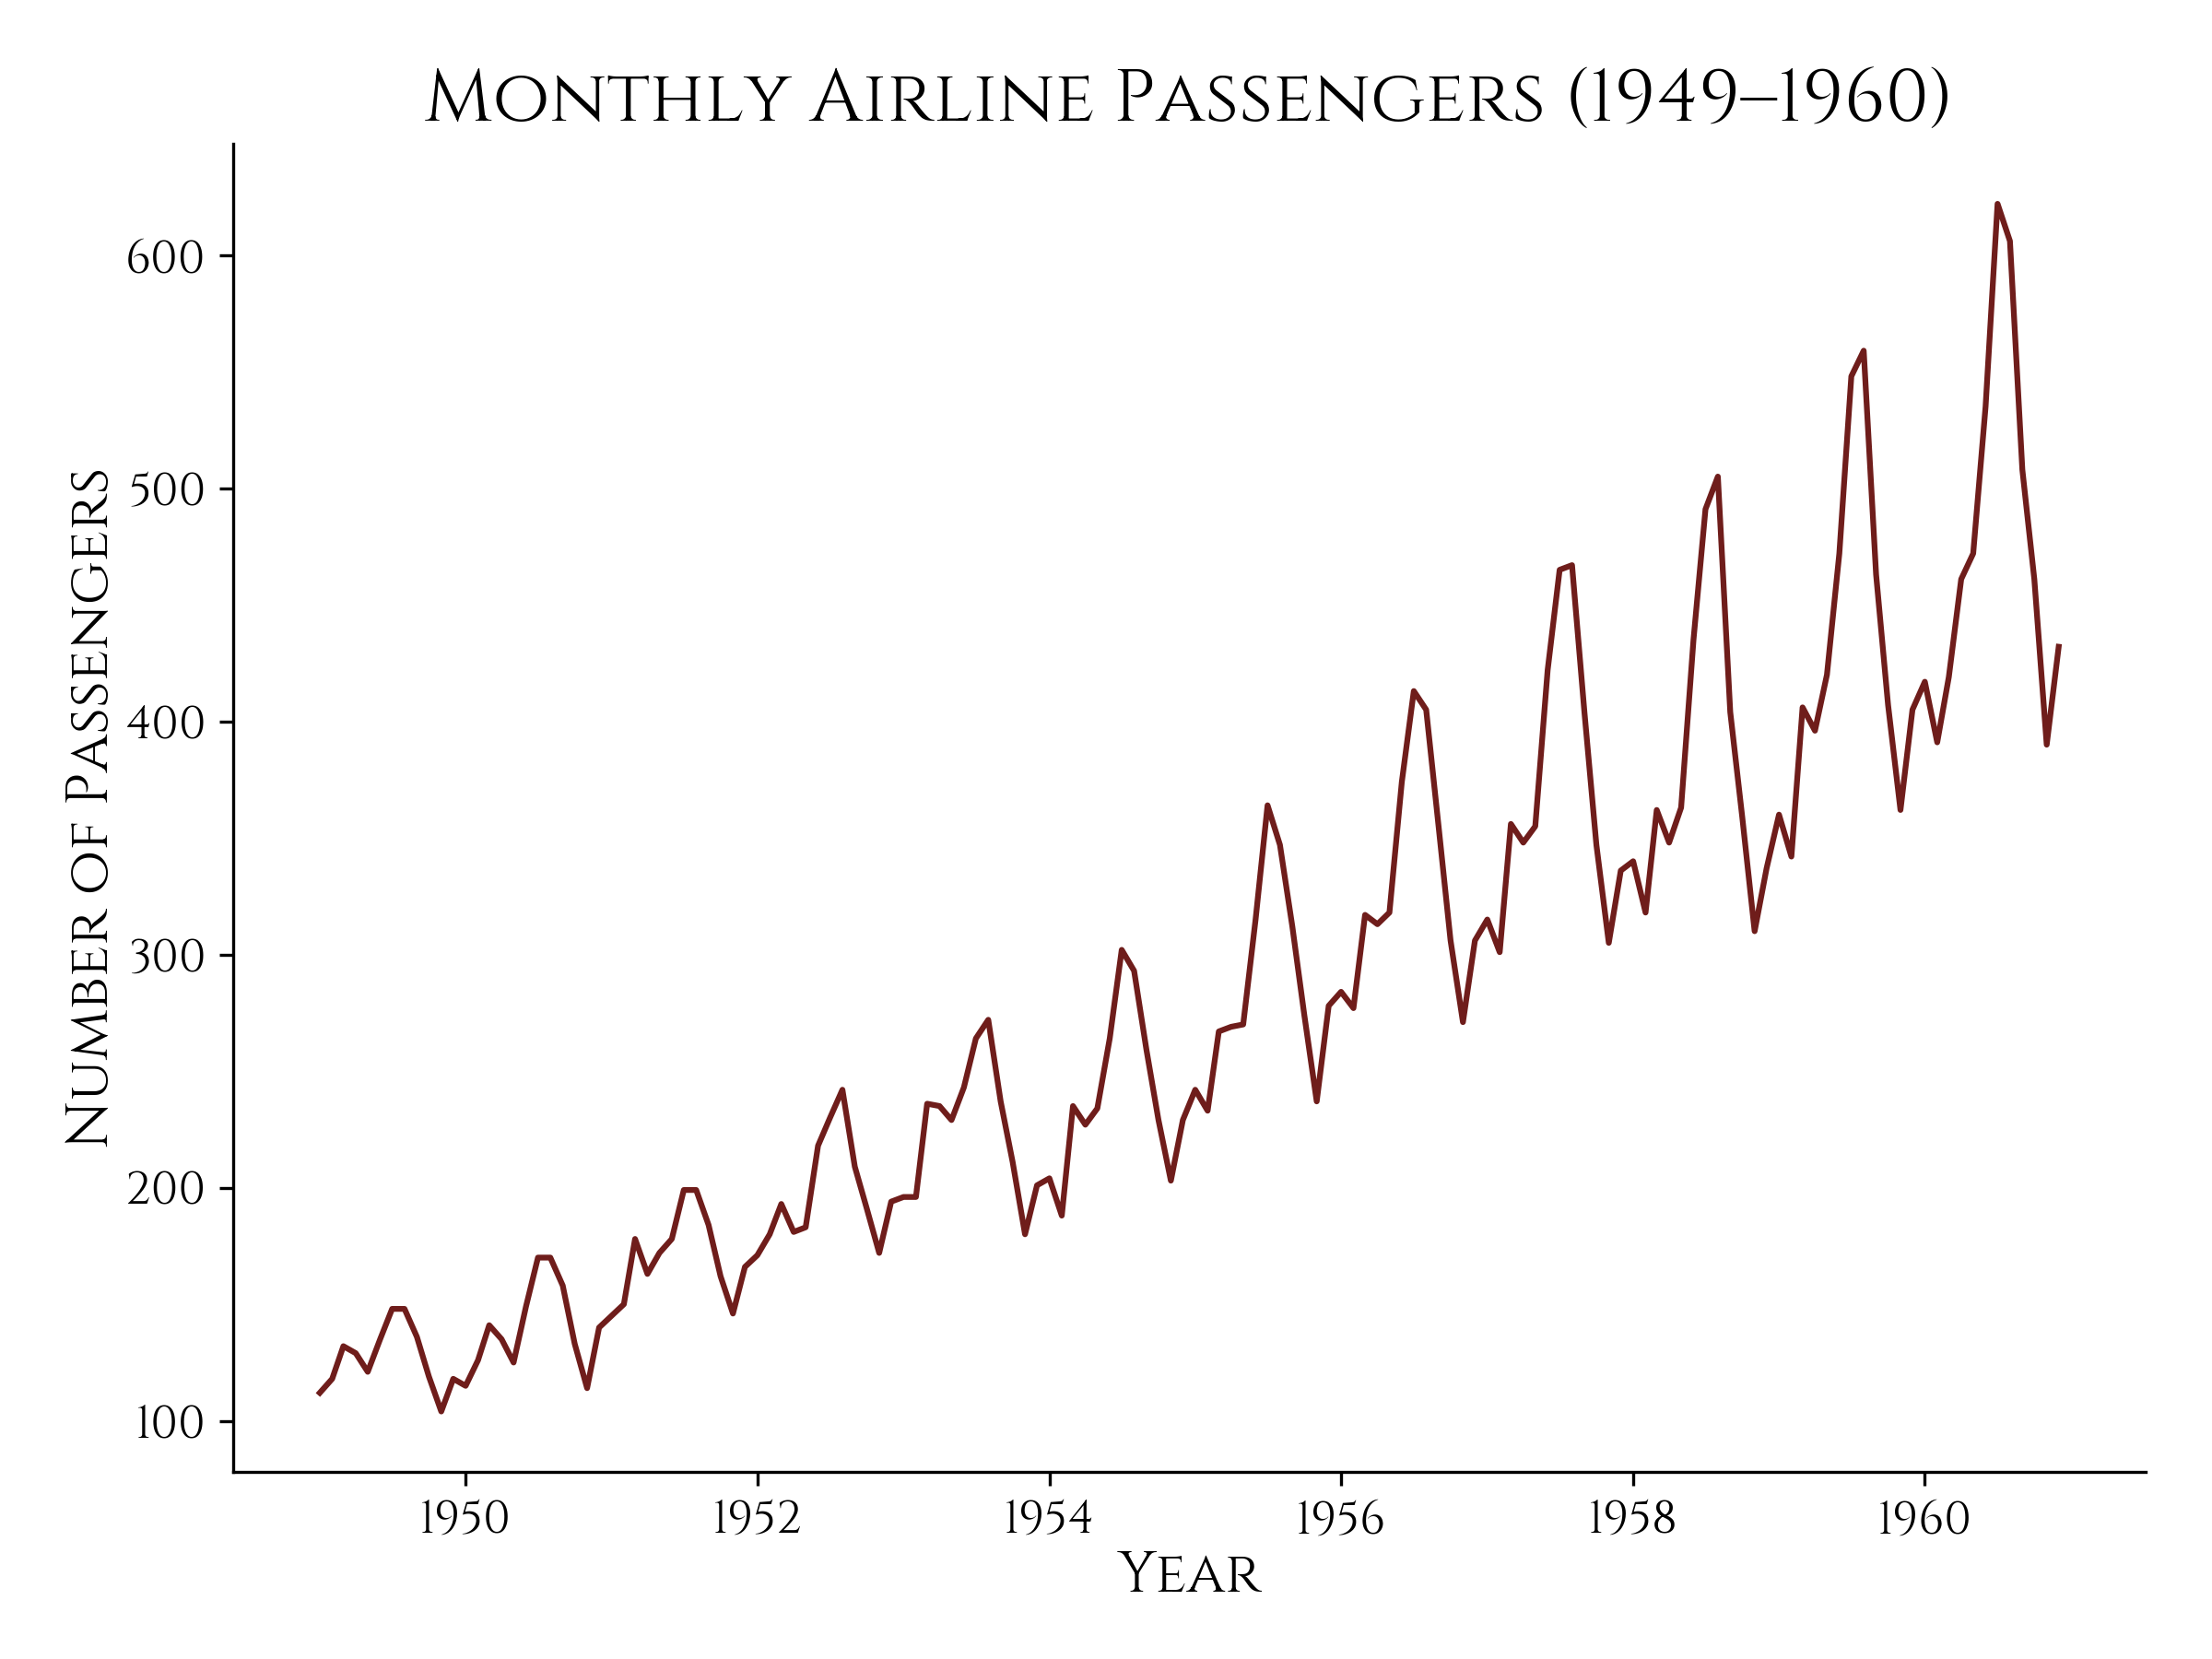
\includegraphics[width=1\textwidth, height=1\textheight, keepaspectratio]{time_series_example_airline_small}
        \captionof{figure}{Ежемесячное количество пассажиров авиалиний с 1949 по 
        1960 года до преобразования Бокса-Кокса. Построено программой по адресу 
        (листинг \ref{lst:time_series_example_airline_small}).}
        \label{fig:time_series_example_airline_small2}
    \end{minipage}
    \hfill
    \begin{minipage}{0.45\textwidth}
        \centering
        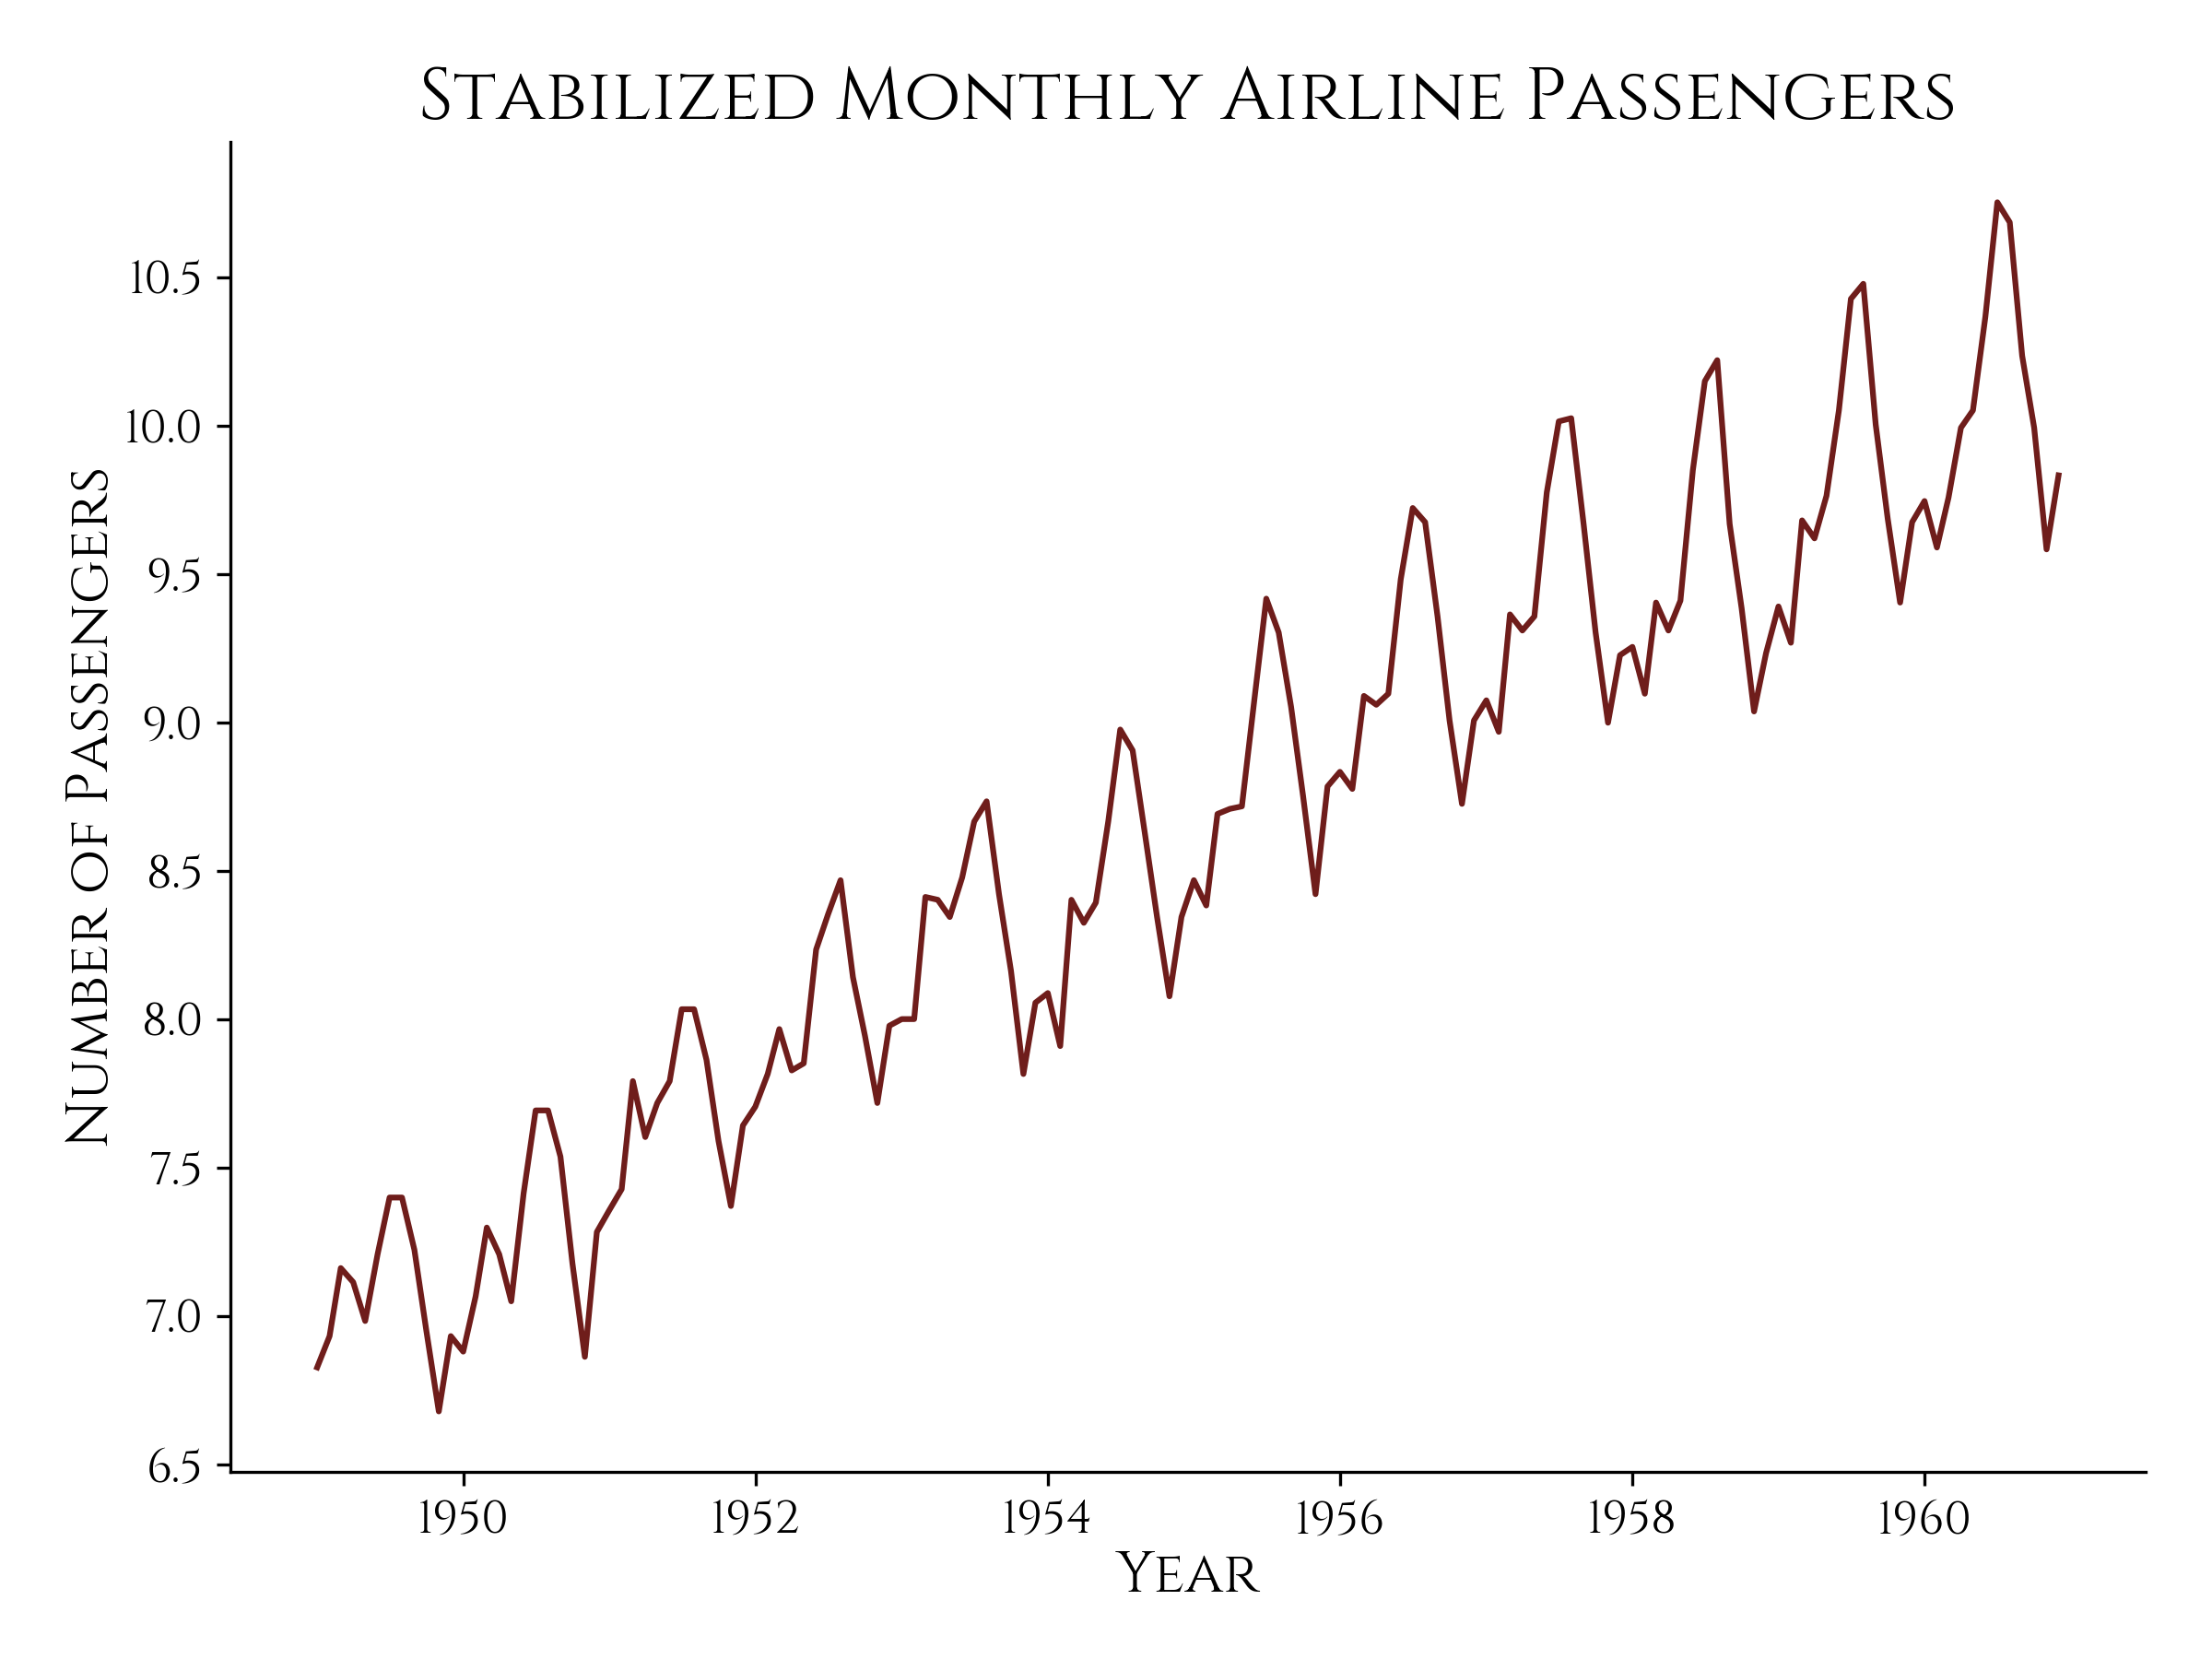
\includegraphics[width=1\textwidth, height=1\textheight, keepaspectratio]{time_series_example_airline_boxcox_small}
        \captionof{figure}{Ежемесячное количество пассажиров авиалиний с 1949 по 
        1960 года после преобразования Бокса-Кокса. Построено программой по адресу 
        (листинг \ref{lst:time_series_example_airline_boxcox_small}).}
        \label{fig:time_series_example_airline_boxcox_small}
    \end{minipage}
\end{center}

Видно, что после применения преобразования Бокса-Кокса размах колебаний в начале и
конце ряда становится очень похожим, и дисперсия примерно стабилизируется. 

\subsection{Модели прогнозирования временных рядов}

Основное внимание в данной работе уделяется применению методов 
машинного обучения, в особенности моделей глубокого обучения, 
для задачи прогнозирования временных рядов. Однако, прежде чем перейти к 
описанию этих современных подходов, целесообразно изучить традиционные 
статистические методы. Это необходимо, поскольку многие концепции 
анализа временных рядов, используемые в классических моделях, 
остаются актуальными и при разработке нейросетевых архитектур, а 
сами классические методы служат отправной точкой для оценки 
производительности новых алгоритмов.

% maybe take a look at multivariate time series

% include "White Noise" chapter 
% include model diagnosics

% use walk-forward validation to evaluate the models

\subsubsection{Белый шум}

Основным строительным блоком для многих дальнейших процессов 
послужит последовательность $\left\{ \varepsilon_t \right\}$, 
элементы которой имеют нулевые среднее и дисперсию $\sigma^2$,

\begin{gather}
    \mathbb{E}\left[ \varepsilon_t \right] = 0 \label{eq:1} \\
    \mathbb{E} \left[ \varepsilon_t^2 \right] = \sigma^2, \label{eq:2}
\end{gather}

и для которой $\varepsilon$ некоррелированны во времени:

\begin{equation}
    \mathbb{E} \left[ \varepsilon_t \varepsilon_\tau \right] = 0, \qquad t \neq \tau. \label{eq:3}
\end{equation}

Процесс, удовлетворяющий условиям \eqref{eq:1} - \eqref{eq:3} называется \textbf{белым шумом}
(white noise process).

Иногда условие \eqref{eq:3} заменяют более сильным: $\varepsilon$ 
независимы во времени:

\begin{equation}
    \varepsilon_t, \varepsilon_\tau \quad \text{независимы при} \quad t \neq \tau. \label{eq:4}
\end{equation}

Процесс, удовлетворяющий условиям \eqref{eq:1} - \eqref{eq:4} называется \textbf{независимым 
белым шумом} (independent white noise process).

Наконец, если помимо условий \eqref{eq:1} - \eqref{eq:4}, также выполняется:

\begin{equation*}
    \varepsilon_t \sim N(0, \sigma^2),
\end{equation*}

то процесс называют \textbf{Гауссовым белым шумом} (Gaussian white noise 
process) \cite{TSA_Hamilton}.

\paragraph{Диагностика модели}

Диагностика модели - важная область в прогнозировании временных рядов. 
Ожидается, что данные временного ряда содержат некоторую компоненту 
белого шума поверх сигнала, сгенерированого, лежащим в основе, процессом. 
Например: 

\begin{equation*}
    y(t) = signal(t) + noise(t)
\end{equation*}

Предсказания модели прогнозирования временного ряда можно собрать и 
проанализировать. Ряд ошибок прогноза в идеале должен быть белым шумом. 
Когда ошибки прогноза удовлетворяют условиям белого шума, это значит, 
что прогнозируюущая модель вобрала в себя всю информацию из сигнала. 
Всё что осталось - случайные колебания, которые нельзя смоделировать. 
То, что предсказания модели не представляют собой белый шум, 
свидетельствует о том, что возможно дальнейшее усовершенствование 
модели прогнозирования \cite{Forecasting_Brownlee}.

\subsubsection{Скользящее среднее (MA)}

Пусть $\left\{ \varepsilon_t \right\}$ - белый шум, удовлетворяющий условиям 
\eqref{eq:1} - \eqref{eq:3}, то процесс:
\begin{equation*}
    X_t = \mu + \varepsilon_t + \theta_1 \varepsilon_{t-1} + 
    \theta_2 \varepsilon_{t-2} + ... + \theta_q \varepsilon_{t-q},
\end{equation*}

где $\mu$ - среднее всего ряда, $(\theta_1, \theta_2, ..., \theta_q)$ - 
весовые коэффициенты, называют \textbf{скользящим средним} порядка $q$ 
(moving average process of order $q$), который часто 
обозначают как \text{MA}($q$). \textit{Не путать с простым 
скользящим средним (simple moving average or moving average smoothing)}.

Некоторые источники опускают параметр $\mu$, так как подразумевают, что ряд 
центрирован ($z_t = X_t - \mu$) \cite{TSA_Box}.

Нередко на практике встречаются и частные случаи данной модели \text{MA}(1) и 
\text{MA}(2):
\begin{align*}
    \text{MA}(1) &: X_t = \mu + \varepsilon_t + \theta_1 \varepsilon_{t-1} \\
    \text{MA}(2) &: X_t = \mu + \varepsilon_t + \theta_1 \varepsilon_{t-1} + \theta_2 \varepsilon_{t-2}
\end{align*}

\subsubsection{AR}

\subsubsection{ARMA}

\subsubsection{ARIMA}

\subsubsection{SARMA}

\subsubsection{SARIMA}

\subsubsection{GARCH}

% MA (Moving Average)

% AR (Autoregressive)

% ARMA (Autoregressive Moving Average)

% ARIMA (Autoregressive Integrated Moving Average)

% SARMA (Seasonal ARMA)

% SARIMA (Seasonal ARIMA)

% GARCH

\subsubsection{Обучение с учителем}

Задачу прогнозирования временных рядов можно переформулировать как 
задачу обучения с учителем. Подобная переформулировка открывает 
доступ к целому набору как линейных, так и нелинейных алгоритмов 
машинного обучения для решения поставленной задачи. \\

...

% "Deep Learning for Time Series Forecasting" by Jason Brownlee

% RNNs (Recurrent Neural Networks) (можно чуть чуть написать и сказать, что затронем 
% подробнее в следующей главе)

% LSTM (Long Short-Term Memory) (может пока не трогать, тк это модификация RNN)

% GRU (может пока не трогать, тк это модификация RNN)
